\documentclass[11pt]{article}


\usepackage{tkz-euclide}
%\usepackage{tkz-base}
%\usetikzlibrary{calc,patterns,angles,quotes,babel}
\usepackage{tkz-euclide}
\usepackage{pgfplots}
\usetkzobj{all}
\usetikzlibrary{shapes.geometric}
\usepackage{amssymb}

\usepgflibrary{arrows}
\usetikzlibrary{arrows} 
\pgfplotsset{compat=newest}
\begin{document}
\section{Module 1: Elementaire rekenvaardigheden A}
%\begin{center}
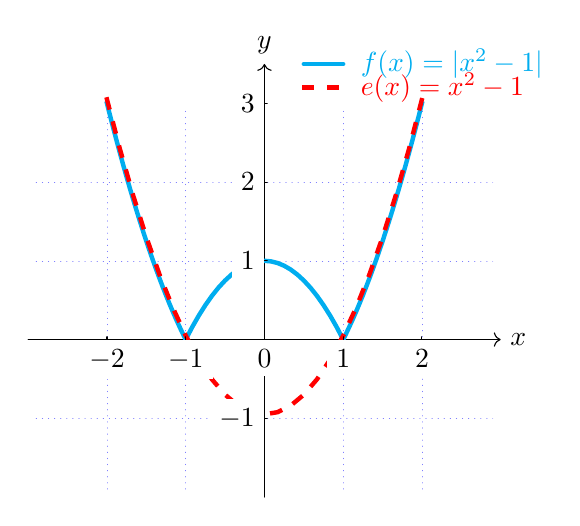
\begin{tikzpicture}[scale=1,cap=round]

% Styles
\tikzstyle{axes}=[]
\tikzstyle help lines=[color=blue!50,very thin,dotted]

% grid
\draw[style=help lines,step=1cm] (-2.9,-1.9) grid (2.9,2.9);


\draw[->] (-3,0) -- (3,0) node[right] {$x$};
\draw[->] (0,-2) -- (0,3.5) node[above] {$y$};

%\draw[fill,cyan](1,1)circle [radius=0.025];

\draw[cyan,cap=rect,ultra thick, domain=-2:-1] plot (\x, {\x*\x-1});

\draw[cyan,cap=rect,ultra thick, domain=-1:1] plot (\x, {-1*(\x*\x-1)});

\draw[cyan,cap=rect,ultra thick, domain=1:2] plot (\x, {\x*\x-1}) node[above, right]{};

\draw[red,cap=rect, loosely dashed, ultra thick, domain=-2:2] plot (\x, {(\x*\x-1)+0.05}) node[above,yshift=-.7cm, right]{};

%legende
\tkzDefPoint(0.5,3.5){A}
\tkzDefPoint(1,3.5){B}
\tkzLabelPoint[right,xshift=+0.1cm](B){${\color{cyan}f(x)=|x^2-1|}$}
\tkzDrawSegment[cyan,ultra thick](A,B)

\tkzDefPoint(0.5,3.2){C}
\tkzDefPoint(1,3.2){D}
\tkzLabelPoint[right,xshift=+0.1cm](D){${\color{red}e(x)=x^2-1}$}
\tkzDrawSegment[red,cap=rect, loosely dashed, ultra thick](C,D)



%getallen op de x-as en lijntjes   
\foreach \x/\xtext in {-2,-1,0, 1,2}
	\draw[xshift=\x cm] (0pt,1pt) -- (0pt,0pt) node[below,fill=white]
	{$\xtext$};,3
	
%getallen op de y-as en lijntjes  
%BEGIN LUS
\foreach \y/\ytext in {-1,1,2,3}
	\draw[yshift=\y cm] (1pt,0pt) -- (0pt,0pt) node[left,fill=white]
	{$\ytext$}; %EINDE LUS



\end{tikzpicture}
\end{center}

%\tikzsetfigurename{Fig_module_1_1_6_parRegelSom}
\begin{center}
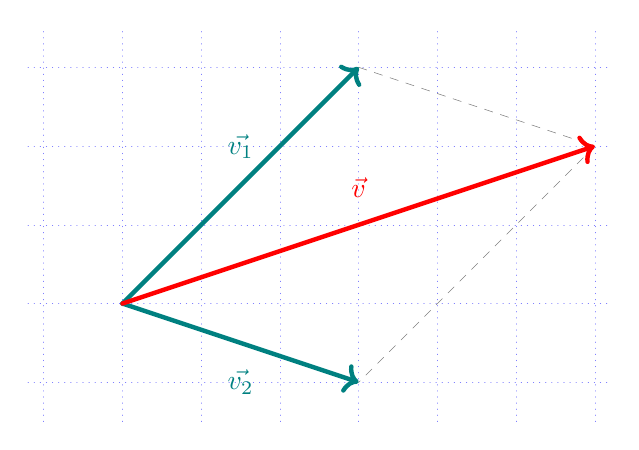
\begin{tikzpicture}[scale=1,cap=round]

% Styles
\tikzstyle{axes}=[]
\tikzstyle help lines=[color=blue!50,very thin,dotted]

% grid
\draw[style=help lines,step=1cm] (-1.2,-1.5) grid (6.2,3.5);



\tkzDefPoint(3,3){A}
\tkzDefPoint(6,2){B}
\tkzDefPoint(3,-1){C}
%\tkzDefPoint(1,1){D}
%\tkzDefPoint(2,2){E}
\tkzDrawSegment[gray,dashed,cap=rect](A,B)
\tkzDrawSegment[gray,dashed,cap=rect](B,C)


\draw[->,teal,ultra thick] (0,0) -- (3,3) node[pos=0.5,above,yshift=+0.2cm] {${\Huge\vec{v_1}}$};
\draw[->,teal,ultra thick] (0,0) -- (3,-1) node[pos=0.5,below,yshift=-0.2cm] {$\vec{v_2}$};
\draw[->,red,ultra thick] (0,0) -- (6,2) node[pos=0.5,above,yshift=+0.2cm] {$\vec{v}$};


\end{tikzpicture}
\end{center}

%\begin{center}
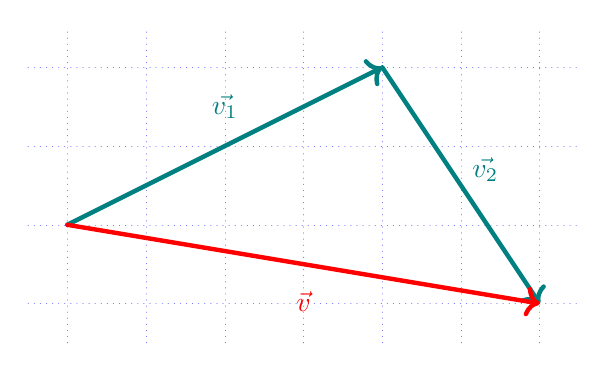
\begin{tikzpicture}[scale=1,cap=round]

% Styles
\tikzstyle{axes}=[]
\tikzstyle help lines=[color=blue!50,very thin,dotted]

% grid
\draw[style=help lines,step=1cm] (-.5,-1.5) grid (6.5,2.5);



\draw[->,teal,ultra thick] (0,0) -- (4,2) node[pos=0.5,above,yshift=+0.2cm] {${\Huge\vec{v_1}}$};
\draw[->,teal,ultra thick] (4,2) -- (6,-1) node[pos=0.5,above,right,yshift=+0.2cm] {$\vec{v_2}$};
\draw[->,red,ultra thick] (0,0) -- (6,-1) node[pos=0.5,below,yshift=-0.2cm] {$\vec{v}$};


\end{tikzpicture}
\end{center}


%\begin{center}
	\begin{tikzpicture}
	%grid
	%\draw[step=1cm,gray,very thin,dotted] (-5,-5) grid 5,5);
	
	\draw[style=help lines,step=0.5cm,gray, very thin, dotted] (-5,-5) grid (5,5);
	%x-as 
	\draw[->] (-5,0)--(5,0) node[anchor=south,left,yshift=0.2cm]{$x$};
	
	%y-as
	\draw[->] (0,-5)--(0,5) node[anchor=south,left]{$y$};
		
	
	\tkzDefPoint(0,0){S}
	\tkzDefPoint(1,0){x1}
	\tkzDefPoint(0,1){y1}
	
	\tkzDefPoint(-3,0){A1}
	\tkzDefPoint(0,-1){A2}
	
	\tkzDefPoint(-3,-1){A}
	
	\tkzDefPoint(1,0){B1}
	\tkzDefPoint(0,4){B2}
	
	\tkzDefPoint(1,4){B}
	
	\tkzDefPoint(2,0){C1}
	\tkzDefPoint(0,-3){C2}
	
	\tkzDefPoint(2,-3){C}
	
	\tkzLabelPoint[below,xshift=-0.1cm](S){$0$}
	\tkzLabelPoint[right,yshift=-0.3cm](S){$O$}
	
	\tkzLabelPoint[below](x1){$1$}
	\tkzLabelPoint[left](y1){$1$}
	
	\tkzLabelPoint[left,yshift=0.2cm](A){$A$}
	\tkzLabelPoint[right,yshift=0.2cm](B){$B$}
	\tkzLabelPoint[right,yshift=0.2cm](C){$C$}
	
	\tkzLabelPoint[above](A1){$-3$}
	\tkzLabelPoint[right](A2){$-1$}
	
 	\tkzLabelPoint[below](B1){$-1$}
	\tkzLabelPoint[left](B2){$4$}
	
	\tkzLabelPoint[above](C1){$2$}
	\tkzLabelPoint[left](C2){$-3$}	
	
	\tkzDrawSegment[black!60!black,dotted](A1,A)
	\tkzDrawSegment[black!60!black,dotted](A2,A)
	\tkzDrawSegment[black!60!black,dotted](B1,B)
	\tkzDrawSegment[black!60!black,dotted](B2,B)
	\tkzDrawSegment[black!60!black,dotted](C1,C)
	\tkzDrawSegment[black!60!black,dotted](C2,C)
	
	\tkzDrawSegment[black!60!black](A,C)
	\tkzDrawSegment[black!60!black](A,B)
	\tkzDrawSegment[black!60!black](B,C)
	
	\foreach \n in {S,x1,y1,A1,A2,A,B1,B2,B,C1,C2,C}
	\node at (\n)[circle,fill,inner sep=1.5pt]{};

	\end{tikzpicture}
\end{center}


\newpage
\begin{center}
\begin{tikzpicture}[scale=2,cap=round]

% Styles
\tikzstyle{axes}=[]
\tikzstyle help lines=[color=blue!50,very thin,dotted]

% grid
\draw[style=help lines,step=0.5cm] (-2.9,-2.9) grid (2.9,2.9);

%\draw (0,0) circle (2cm);

\draw[->] (-3,0) -- (3,0) node[right] {$x$};
\draw[->] (0,-3) -- (0,3) node[above] {$y$};

%getallen op de x-as én lijntje?  
\foreach \x/\xtext in {-3,-2,-1, -.5/-\frac{1}{2}, 1,2,2.5}
\draw[xshift=\x cm] (0pt,1pt) -- (0pt,-1pt) node[below,fill=white]
{$\xtext$};
%getallen op de y-as én lijntje? 
\foreach \y/\ytext in {-3,-2,-1, -.5/-\frac{1}{2}, .5/\frac{1}{2}, 1,2}
\draw[yshift=\y cm] (1pt,0pt) -- (-1pt,0pt) node[left,fill=white]
{$\ytext$};



\end{tikzpicture}
\end{center}
\newpage

\begin{tikzpicture}[scale=3,cap=round]
% Local definitions
\def\costhirty{0.8660256}

% Colors
\colorlet{anglecolor}{green!50!black}
\colorlet{sincolor}{red}
\colorlet{tancolor}{orange!80!black}
\colorlet{coscolor}{blue}

% Styles
\tikzstyle{axes}=[]
\tikzstyle{important line}=[very thick]
\tikzstyle{information text}=[rounded corners,fill=red!10,inner sep=1ex]

% The graphic
\draw[style=help lines,step=0.5cm,very thin, gray, dotted] (-1.4,-1.4) grid (1.4,1.4);

\draw (0,0) circle (1cm);

\begin{scope}[style=axes]
\draw[->] (-1.5,0) -- (1.5,0) node[right] {$x$};
\draw[->] (0,-1.5) -- (0,1.5) node[above] {$y$};

\foreach \x/\xtext in {-1, -.5/-\frac{1}{2}, 1}
\draw[xshift=\x cm] (0pt,1pt) -- (0pt,-1pt) node[below,fill=white]
{$\xtext$};

\foreach \y/\ytext in {-1, -.5/-\frac{1}{2}, .5/\frac{1}{2}, 1}
\draw[yshift=\y cm] (1pt,0pt) -- (-1pt,0pt) node[left,fill=white]
{$\ytext$};
\end{scope}

\filldraw[fill=green!20,draw=anglecolor] (0,0) -- (3mm,0pt) arc(0:30:3mm);
\draw (15:2mm) node[anglecolor] {$\alpha$};

\draw[style=important line,sincolor]
(30:1cm) -- node[left=1pt,fill=white] {$\sin \alpha$} +(0,-.5);

\draw[style=important line,coscolor]
(0,0) -- node[below=2pt,fill=white] {$\cos \alpha$} (\costhirty,0);

\draw[style=important line,tancolor] (1,0) --
node [right=1pt,fill=white]
{
	$\displaystyle \tan \alpha \color{black}=
	\frac{{\color{sincolor}\sin \alpha}}{\color{coscolor}\cos \alpha}$
} (intersection of 0,0--30:1cm and 1,0--1,1) coordinate (t);

\draw (0,0) -- (t);

%\draw[xshift=1.85cm] node [right,text width=6cm,style=information text]
%{
%	The {\color{anglecolor} angle $\alpha$} is $30^\circ$ in the
%	example ($\pi/6$ in radians). The {\color{sincolor}sine of
%		$\alpha$}, which is the height of the red line, is
%	\[
%	{\color{sincolor} \sin \alpha} = 1/2.
%	\]
%	By the Theorem of Pythagoras we have ${\color{coscolor}\cos^2 \alpha} +
%	{\color{sincolor}\sin^2\alpha} =1$. Thus the length of the blue
%	line, which is the {\color{coscolor}cosine of $\alpha$}, must be
%	\[
%	{\color{coscolor}\cos\alpha} = \sqrt{1 - 1/4} = \textstyle
%	\frac{1}{2} \sqrt 3.
%	\]%
%	This shows that {\color{tancolor}$\tan \alpha$}, which is the
%	height of the orange line, is
%	\[
%	{\color{tancolor}\tan\alpha} = \frac{{\color{sincolor}\sin
%			\alpha}}{\color{coscolor}\cos \alpha} = 1/\sqrt 3.
%	\]%
%};
\end{tikzpicture}

%\begin{center}
\begin{tikzpicture}[scale=1,cap=round]


% Styles
\tikzstyle{axes}=[]
\tikzstyle help lines=[color=blue!50,very thin,dotted]

% grid
\draw[style=help lines,step=1cm] (-2.9,-2.9) grid (2.9,2.9);


\draw[->] (-3,0) -- (3,0) node[right] {$x$};
\draw[->] (0,-3) -- (0,3) node[above] {$y$};

\draw[thick, dashed, cyan,domain=-2:2] plot(\x, \x)  node[right]{$f(x)=x$};
%\draw[fill,cyan](1,1)circle [radius=0.025];

\tkzDefPoint(-2,-2){A}
\tkzDefPoint(-1,-1){B}
\tkzDefPoint(0,0){C}
\tkzDefPoint(1,1){D}
\tkzDefPoint(2,2){E}


\foreach \n in {A,B,C,D,E}
\node at (\n)[circle,cyan,fill,inner sep=1.5pt]{};

%getallen op de x-as en lijntjes   
\foreach \x/\xtext in {-3,-2,-1,0, 1,2,3}
	\draw[xshift=\x cm] (0pt,1pt) -- (0pt,0pt) node[below,fill=white]
	{$\xtext$};
	
%getallen op de y-as en lijntjes  
%BEGIN LUS
\foreach \y/\ytext in {-3,-2,-1,1,2}
	\draw[yshift=\y cm] (1pt,0pt) -- (0pt,0pt) node[left,fill=white]
	{$\ytext$}; %EINDE LUS
\end{tikzpicture}
\end{center}


%\begin{center}
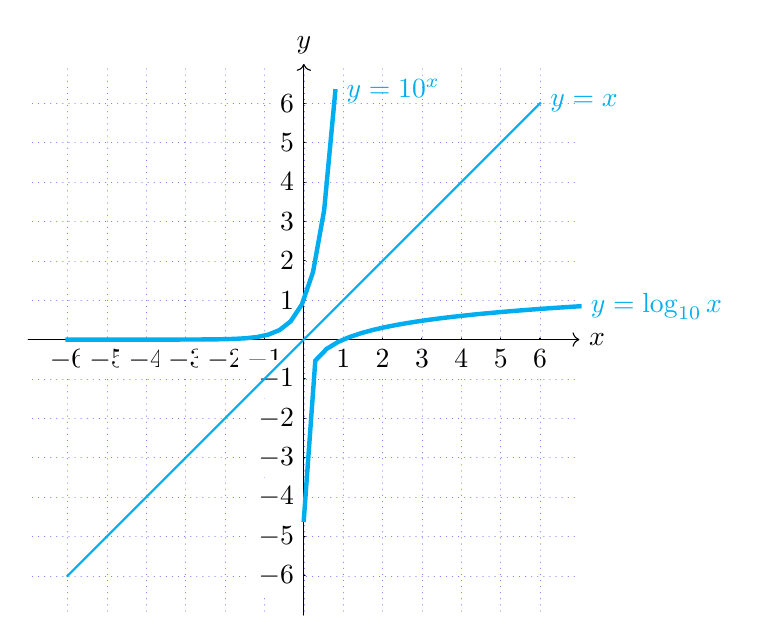
\begin{tikzpicture}[scale=0.5,cap=round]

% Styles
\tikzstyle{axes}=[]
\tikzstyle help lines=[color=blue!50,very thin,dotted]


%%%%%%%%%%%%%%%%%%%%%%%%%%%%%%%%
%		GRID
%%%%%%%%%%%%%%%%%%%%%%%%%%%%%%%%

\draw[style=help lines,step=1cm] (-6.9,-6.9) grid (6.9,6.9);

%%%%%%%%%%%%%%%%%%%%%%%%%%%%%%%%
%		ASSENSTELSEL
%%%%%%%%%%%%%%%%%%%%%%%%%%%%%%%%

\draw[->] (-7,0) -- (7,0) node[right] {$x$};
\draw[->] (0,-7) -- (0,7) node[above] {$y$};

%\draw[fill,cyan](1,1)circle [radius=0.025];

%\draw[red,cap=rect, loosely dashed, ultra thick, domain=-2:2] plot (\x, {(\x*\x-1)+0.05}) node[above,yshift=-.7cm, right]{};

%%%%%%%%%%%%%%%%%%%%%%%%%%%%%%%%
%legende
%%%%%%%%%%%%%%%%%%%%%%%%%%%%%%%%
%\tkzDefPoint(0.5,3.5){A}
%\tkzDefPoint(1,3.5){B}
%\tkzLabelPoint[right,xshift=+0.1cm](B){${\color{cyan}f(x)=|x^2-1|}$}
%\tkzDrawSegment[cyan,ultra thick](A,B)

%\tkzDefPoint(0.5,3.2){C}
%\tkzDefPoint(1,3.2){D}
%\tkzLabelPoint[right,xshift=+0.1cm](D){${\color{red}e(x)=x^2-1}$}
%\tkzDrawSegment[red,cap=rect, loosely dashed, ultra thick](C,D)


%%%%%%%%%%%%%%%%%%%%%%%%%%%%%%%%
%getallen op de x-as en lijntjes
%%%%%%%%%%%%%%%%%%%%%%%%%%%%%%%%   
\foreach \x/\xtext in {-6,-5,-4,-3,-2,-1,1,2,3,4,5,6}
	\draw[xshift=\x cm] (0pt,1pt) -- (0pt,0pt) node[below,fill=white]
	{$\xtext$};,3
	
%getallen op de y-as en lijntjes  
%BEGIN LUS
\foreach \y/\ytext in {-6,-5,-4,-3,-2,-1,1,2,3,4,5,6}
	\draw[yshift=\y cm] (1pt,0pt) -- (0pt,0pt) node[left,fill=white]
	{$\ytext$}; %EINDE LUS



%%%%%%%%%%%%%%%%%%%%%%%%%%%%%%%%
%		GRAFIEKEN
%%%%%%%%%%%%%%%%%%%%%%%%%%%%%%%%
\draw[cyan,cap=rect,thick, domain=-6:6] plot (\x, \x) node[above, right]{${\color{cyan}y=x}$};

\draw[cyan,cap=rect,ultra thick, domain=0.00001:7] plot (\x, {log10{\x}}) node[above, right]{${\color{cyan}y=\log_{10}{x}}$};

\draw[cyan,cap=rect,ultra thick, domain=-6:.8] plot (\x, {pow(10,\x)}) node[above, right]{${\color{cyan}y=10^x}$};


\end{tikzpicture}
\end{center}


%\tikzsetfigurename{Fig_module_1_2_9_logFunc2}
\begin{center}
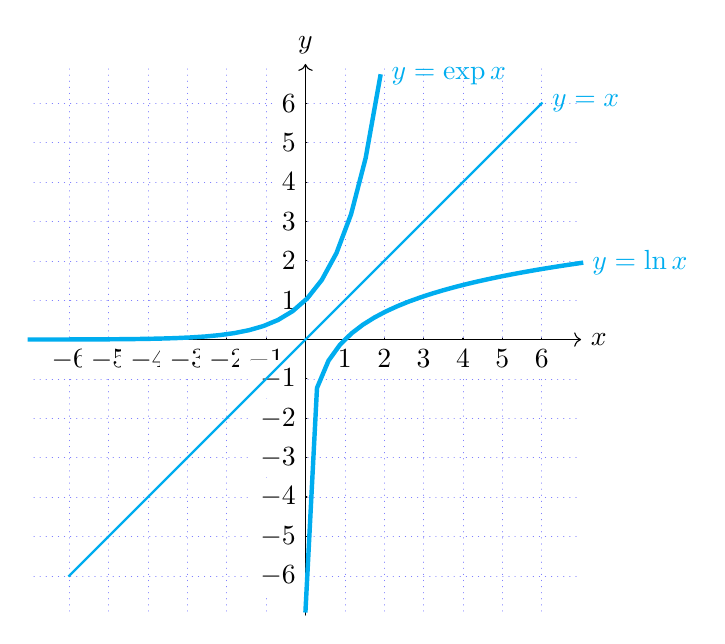
\begin{tikzpicture}[scale=0.5,cap=round]

% Styles
\tikzstyle{axes}=[]
\tikzstyle help lines=[color=blue!50,very thin,dotted]


%%%%%%%%%%%%%%%%%%%%%%%%%%%%%%%%
%		GRID
%%%%%%%%%%%%%%%%%%%%%%%%%%%%%%%%

\draw[style=help lines,step=1cm] (-6.9,-6.9) grid (6.9,6.9);

%%%%%%%%%%%%%%%%%%%%%%%%%%%%%%%%
%		ASSENSTELSEL
%%%%%%%%%%%%%%%%%%%%%%%%%%%%%%%%

\draw[->] (-7,0) -- (7,0) node[right] {$x$};
\draw[->] (0,-7) -- (0,7) node[above] {$y$};

%\draw[fill,cyan](1,1)circle [radius=0.025];

%\draw[red,cap=rect, loosely dashed, ultra thick, domain=-2:2] plot (\x, {(\x*\x-1)+0.05}) node[above,yshift=-.7cm, right]{};

%%%%%%%%%%%%%%%%%%%%%%%%%%%%%%%%
%legende
%%%%%%%%%%%%%%%%%%%%%%%%%%%%%%%%
%\tkzDefPoint(0.5,3.5){A}
%\tkzDefPoint(1,3.5){B}
%\tkzLabelPoint[right,xshift=+0.1cm](B){${\color{cyan}f(x)=|x^2-1|}$}
%\tkzDrawSegment[cyan,ultra thick](A,B)

%\tkzDefPoint(0.5,3.2){C}
%\tkzDefPoint(1,3.2){D}
%\tkzLabelPoint[right,xshift=+0.1cm](D){${\color{red}e(x)=x^2-1}$}
%\tkzDrawSegment[red,cap=rect, loosely dashed, ultra thick](C,D)


%%%%%%%%%%%%%%%%%%%%%%%%%%%%%%%%
%getallen op de x-as en lijntjes
%%%%%%%%%%%%%%%%%%%%%%%%%%%%%%%%   
\foreach \x/\xtext in {-6,-5,-4,-3,-2,-1,1,2,3,4,5,6}
	\draw[xshift=\x cm] (0pt,1pt) -- (0pt,0pt) node[below,fill=white]
	{$\xtext$};,3
	
%getallen op de y-as en lijntjes  
%BEGIN LUS
\foreach \y/\ytext in {-6,-5,-4,-3,-2,-1,1,2,3,4,5,6}
	\draw[yshift=\y cm] (1pt,0pt) -- (0pt,0pt) node[left,fill=white]
	{$\ytext$}; %EINDE LUS



%%%%%%%%%%%%%%%%%%%%%%%%%%%%%%%%
%		GRAFIEKEN
%%%%%%%%%%%%%%%%%%%%%%%%%%%%%%%%
\draw[cyan,cap=rect,thick, domain=-6:6] plot (\x, \x) node[above, right]{${\color{cyan}y=x}$};

\draw[cyan,cap=rect,ultra thick, domain=0.001:7] plot (\x, {ln{\x}}) node[above, right]{${\color{cyan}y=\ln{x}}$};

\draw[cyan,cap=rect,ultra thick, domain=-7:1.9] plot (\x, {exp{\x}}) node[above, right]{${\color{cyan}y=\exp{x}}$};


\end{tikzpicture}
\end{center}
\newpage
\section{Module 2: Elementaire rekenvaardigheden B}
%\tikzsetfigurename{Fig_module_2_1_2_reele_functies_vb1}
%TODO polynoombenadering uitrekenen > zie cursus Algebra

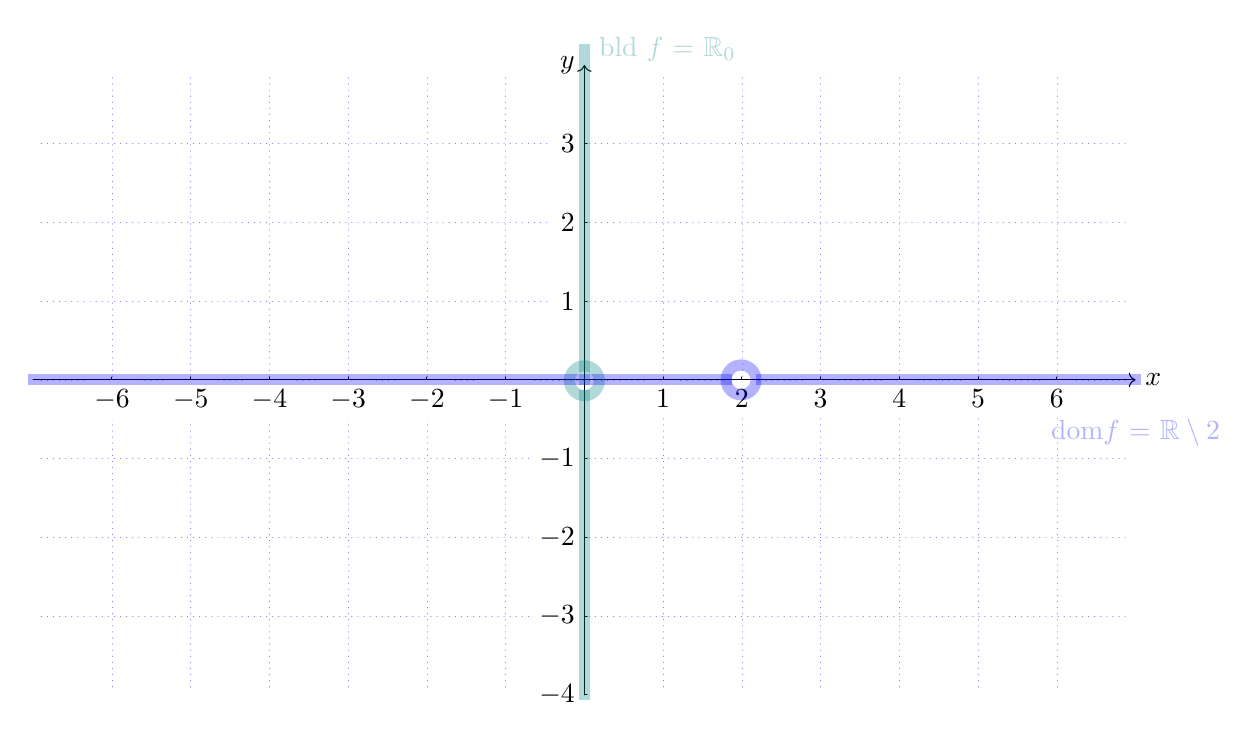
\begin{tikzpicture}[cap=round]

% Styles
\tikzstyle{axes}=[]
\tikzstyle help lines=[color=blue!50,very thin,dotted]


%%%%%%%%%%%%%%%%%%%%%%%%%%%%%%%%
%		GRID
%%%%%%%%%%%%%%%%%%%%%%%%%%%%%%%%

\draw[style=help lines,step=1cm] (-6.9,-3.9) grid (6.9,3.9);



%%%%%%%%%%%%%%%%%%%%%%%%%%%%%%%%
%		ASSENSTELSEL
%%%%%%%%%%%%%%%%%%%%%%%%%%%%%%%%

\draw[->] (-7,0) -- (7,0) node[right] {$x$};
\draw[->] (0,-4) -- (0,4) node[left]{$y$};

%\draw[fill,cyan](1,1)circle [radius=0.025];

%\draw[red,cap=rect, loosely dashed, ultra thick, domain=-2:2] plot (\x, {(\x*\x-1)+0.05}) node[above,yshift=-.7cm, right]{};

%%%%%%%%%%%%%%%%%%%%%%%%%%%%%%%%
%legende
%%%%%%%%%%%%%%%%%%%%%%%%%%%%%%%%
%\tkzDefPoint(0.5,3.5){A}
%\tkzDefPoint(1,3.5){B}
%\tkzLabelPoint[right,xshift=+0.1cm](B){${\color{cyan}f(x)=|x^2-1|}$}
%\tkzDrawSegment[cyan,ultra thick](A,B)

%\tkzDefPoint(0.5,3.2){C}
%\tkzDefPoint(1,3.2){D}
%\tkzLabelPoint[right,xshift=+0.1cm](D){${\color{red}e(x)=x^2-1}$}
%\tkzDrawSegment[red,cap=rect, loosely dashed, ultra thick](C,D)


%%%%%%%%%%%%%%%%%%%%%%%%%%%%%%%%
%getallen op de x-as en lijntjes
%%%%%%%%%%%%%%%%%%%%%%%%%%%%%%%%   
\foreach \x/\xtext in {-6,-5,-4,-3,-2,-1,1,2,3,4,5,6}
	\draw[xshift=\x cm] (0pt,1pt) -- (0pt,0pt) node[below,fill=white]
	{$\xtext$};,3
	
%getallen op de y-as en lijntjes  
%BEGIN LUS
\foreach \y/\ytext in {-4,-3,-2,-1,1,2,3}
	\draw[yshift=\y cm] (1pt,0pt) -- (0pt,0pt) node[left,fill=white]
	{$\ytext$}; %EINDE LUS



%%%%%%%%%%%%%%%%%%%%%%%%%%%%%%%%
%		GRAFIEKEN
%%%%%%%%%%%%%%%%%%%%%%%%%%%%%%%%
%\draw[cyan,cap=rect,thick, domain=-6:6] plot (\x, \x) node[above, right]{${\color{cyan}y=x}$};v

%\draw[cyan,cap=rect,ultra thick, domain=-6:1.75] plot (\x, {(\x-2)^(-1)}) node[above,right]{};


%\draw[cyan,cap=rect,ultra thick, domain=2.25:6] plot (\x, {(\x-2)^(-1)}) node[above,yshift=+0.5cm,left]{$\color{cyan} y=\frac{1}{x-2}$};


%\draw[cyan,cap=rect,ultra thick, domain=-7:1.9] plot (\x, {exp{\x}}) node[above, right]{${\color{cyan}y=\exp{x}}$};

%%%%%%%%%%%%%%%%%%%%%%%%%%%%%%%%
%		MARKERINGEN
%%%%%%%%%%%%%%%%%%%%%%%%%%%%%%%%
%verticale lijn
\draw[-o,line width=4,teal, cap=rect,opacity=0.3] (0,-4) -- (0,0.25) node[right] {};
\draw[line width=4,teal, cap=rect,opacity=0.3] (0,0) -- (0,4.2) node[right] {bld $f$ = $\mathbb{R}_0$};
%horizontale lijn
\draw[arrows=-o,line width=4,blue, cap=rect,opacity=0.3] (-7,0) -- (2.25,0) node[right] {};
\draw[line width=4,blue, cap=rect,opacity=0.3] (2.25,0) -- (7,0) node[below,yshift=-0.3cm] {dom$f$ = $\mathbb{R}  \setminus 2 $};
 
\end{tikzpicture}

%
\begin{center}
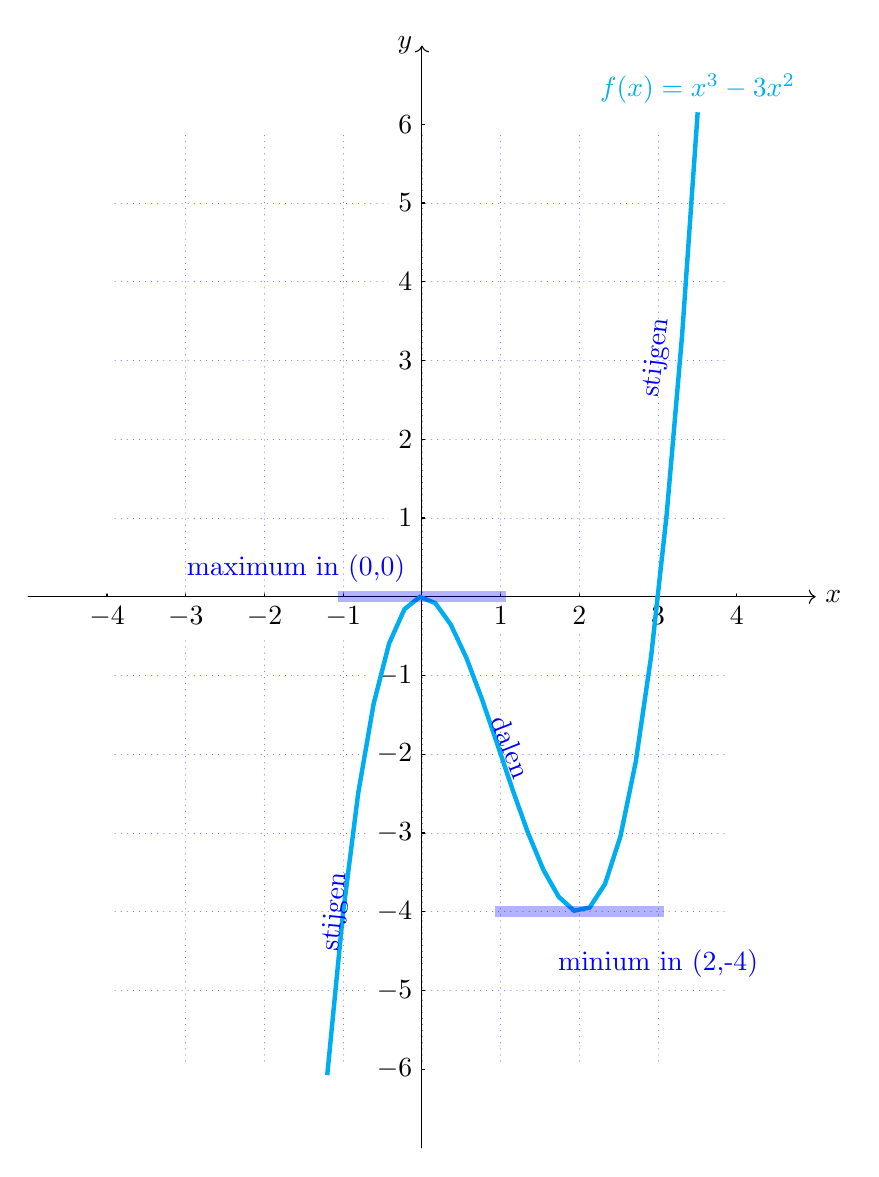
\begin{tikzpicture}[scale=1,cap=round]

% Styles
\tikzstyle{axes}=[]
\tikzstyle help lines=[color=blue!50,very thin,dotted]


%%%%%%%%%%%%%%%%%%%%%%%%%%%%%%%%
%		GRID
%%%%%%%%%%%%%%%%%%%%%%%%%%%%%%%%

\draw[style=help lines,step=1cm] (-3.9,-5.9) grid (3.9,5.9);



%%%%%%%%%%%%%%%%%%%%%%%%%%%%%%%%
%		ASSENSTELSEL
%%%%%%%%%%%%%%%%%%%%%%%%%%%%%%%%

\draw[->] (-5,0) -- (5,0) node[right] {$x$};
\draw[->] (0,-7) -- (0,7) node[left]{$y$};

%\draw[fill,cyan](1,1)circle [radius=0.025];

%\draw[red,cap=rect, loosely dashed, ultra thick, domain=-2:2] plot (\x, {(\x*\x-1)+0.05}) node[above,yshift=-.7cm, right]{};

%%%%%%%%%%%%%%%%%%%%%%%%%%%%%%%%
%legende
%%%%%%%%%%%%%%%%%%%%%%%%%%%%%%%%
%\tkzDefPoint(0.5,3.5){A}
%\tkzDefPoint(1,3.5){B}
%\tkzLabelPoint[right,xshift=+0.1cm](B){${\color{cyan}f(x)=|x^2-1|}$}
%\tkzDrawSegment[cyan,ultra thick](A,B)

%\tkzDefPoint(0.5,3.2){C}
%\tkzDefPoint(1,3.2){D}
%\tkzLabelPoint[right,xshift=+0.1cm](D){${\color{red}e(x)=x^2-1}$}
%\tkzDrawSegment[red,cap=rect, loosely dashed, ultra thick](C,D)


%%%%%%%%%%%%%%%%%%%%%%%%%%%%%%%%
%getallen op de x-as en lijntjes
%%%%%%%%%%%%%%%%%%%%%%%%%%%%%%%%   
\foreach \x/\xtext in {-4,-3,-2,-1,1,2,3,4}
	\draw[xshift=\x cm] (0pt,1pt) -- (0pt,0pt) node[below,fill=white]
	{$\xtext$};,3
	
%getallen op de y-as en lijntjes  
%BEGIN LUS
\foreach \y/\ytext in {-6,-5,-4,-3,-2,-1,1,2,3,4,5,6}
	\draw[yshift=\y cm] (1pt,0pt) -- (0pt,0pt) node[left,fill=white]
	{$\ytext$}; %EINDE LUS



%%%%%%%%%%%%%%%%%%%%%%%%%%%%%%%%
%		GRAFIEKEN
%%%%%%%%%%%%%%%%%%%%%%%%%%%%%%%%
%\draw[cyan,cap=rect,thick, domain=-6:6] plot (\x, \x) node[above, right]{${\color{cyan}y=x}$};

\draw[cyan,cap=rect,ultra thick, domain=-1.2:3.5] plot (\x, {
	pow(\x,3)-3*pow(\x,2)		% <- plaats het functievoorschrift hier
}) node[above]{$f(x)=x^3-3x^2$};

\draw[opacity=0] (-1.2,-5) --(-1,-3) node[opacity=1,blue, midway,sloped]{stijgen};  
\draw[opacity=0] (0.5,-1) --(1.3,-3) node[opacity=1,blue, midway,sloped,above]{dalen};  
\draw[opacity=0] (3,1) --(3.5,5) node[opacity=1,blue, midway,sloped,above]{stijgen};  


%node[blue]{stijgen} 
%\draw[cyan,cap=rect,ultra thick, domain=2.25:6] plot (\x, {(\x-2)^(-1)}) node[above,yshift=+0.5cm,left]{$\color{cyan} y=\frac{1}{x-2}$};


%\draw[cyan,cap=rect,ultra thick, domain=-7:1.9] plot (\x, {exp{\x}}) node[above, right]{${\color{cyan}y=\exp{x}}$};

%%%%%%%%%%%%%%%%%%%%%%%%%%%%%%%%
%		MARKERINGEN
%%%%%%%%%%%%%%%%%%%%%%%%%%%%%%%%
%verticale lijn
%\draw[-o,line width=4,teal, cap=rect,opacity=0.3] (0,-4) -- (0,0.25) node[right] {};
%\draw[line width=4,teal, cap=rect,opacity=0.3] (0,0) -- (0,4.2) node[right] {bld $f$ = $\mathbb{R}_0$};
%horizontale lijn
\draw[line width=4,blue, cap=rect,opacity=0.3] (-1,0) -- (1,0) node[near start,above,xshift=-1.1cm,opacity=1] {maximum in (0,0)};

 
\draw[line width=4,blue, cap=rect,opacity=0.3] (1,-4) -- (3,-4) node[below,yshift=-.3cm,opacity=1] {minium in (2,-4)};
\end{tikzpicture}
\end{center}




\begin{tabular}{ccc}
%\hline
%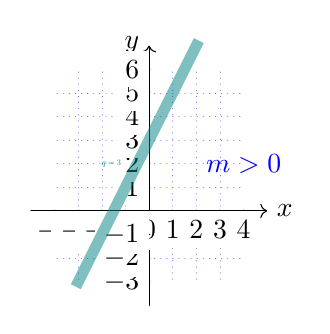
\begin{tikzpicture}[scale=0.3,cap=round]

% Styles
\tikzstyle{axes}=[]
\tikzstyle help lines=[color=blue!50,very thin,dotted]


%%%%%%%%%%%%%%%%%%%%%%%%%%%%%%%%
%		GRID
%%%%%%%%%%%%%%%%%%%%%%%%%%%%%%%%

\draw[style=help lines,step=1cm] (-3.9,-2.9) grid (3.9,5.9);



%%%%%%%%%%%%%%%%%%%%%%%%%%%%%%%%
%		ASSENSTELSEL
%%%%%%%%%%%%%%%%%%%%%%%%%%%%%%%%

\draw[->] (-5,0) -- (5,0) node[right] {$x$};
\draw[->] (0,-4) -- (0,7) node[left]{$y$};

%\draw[fill,cyan](1,1)circle [radius=0.025];

%\draw[red,cap=rect, loosely dashed, ultra thick, domain=-2:2] plot (\x, {(\x*\x-1)+0.05}) node[above,yshift=-.7cm, right]{};

%%%%%%%%%%%%%%%%%%%%%%%%%%%%%%%%
%legende
%%%%%%%%%%%%%%%%%%%%%%%%%%%%%%%%
%\tkzDefPoint(0.5,3.5){A}
%\tkzDefPoint(1,3.5){B}
%\tkzLabelPoint[right,xshift=+0.1cm](B){${\color{cyan}f(x)=|x^2-1|}$}
%\tkzDrawSegment[cyan,ultra thick](A,B)

%\tkzDefPoint(0.5,3.2){C}
%\tkzDefPoint(1,3.2){D}
%\tkzLabelPoint[right,xshift=+0.1cm](D){${\color{red}e(x)=x^2-1}$}
%\tkzDrawSegment[red,cap=rect, loosely dashed, ultra thick](C,D)


%%%%%%%%%%%%%%%%%%%%%%%%%%%%%%%%
%getallen op de x-as en lijntjes
%%%%%%%%%%%%%%%%%%%%%%%%%%%%%%%%   
\foreach \x/\xtext in {-4,-3,-2,-1,0,1,2,3,4}
	\draw[xshift=\x cm] (0pt,1pt) -- (0pt,0pt) node[below,fill=white]
	{$\xtext$};,3
	
%getallen op de y-as en lijntjes  
%BEGIN LUS
\foreach \y/\ytext in {-3,-2,-1,1,2,3,4,5,6}
	\draw[yshift=\y cm] (1pt,0pt) -- (0pt,0pt) node[left,fill=white]
	{$\ytext$}; %EINDE LUS



%%%%%%%%%%%%%%%%%%%%%%%%%%%%%%%%
%		GRAFIEKEN
%%%%%%%%%%%%%%%%%%%%%%%%%%%%%%%%
%\draw[cyan,cap=rect,thick, domain=-6:6] plot (\x, \x) node[above, right]{${\color{cyan}y=x}$};


\draw[teal,cap=rect,line width=4, opacity=.5, domain=-3:2] plot (\x, {
	2*\x + 3 		% <- plaats het functievoorschrift hier
}) node[opacity=1,left,pos=1,xshift=-1cm, yshift=+2cm]{$q=3$};
 
%node[blue]{stijgen} 
%\draw[cyan,cap=rect,ultra thick, domain=2.25:6] plot (\x, {(\x-2)^(-1)}) node[above,yshift=+0.5cm,left]{$\color{cyan} y=\frac{1}{x-2}$};


%\draw[cyan,cap=rect,ultra thick, domain=-7:1.9] plot (\x, {exp{\x}}) node[above, right]{${\color{cyan}y=\exp{x}}$};

%%%%%%%%%%%%%%%%%%%%%%%%%%%%%%%%
%		MARKERINGEN
%%%%%%%%%%%%%%%%%%%%%%%%%%%%%%%%
%verticale lijn
%\draw[-o,line width=4,teal, cap=rect,opacity=0.3] (0,-4) -- (0,0.25) node[right] {};
%\draw[line width=4,teal, cap=rect,opacity=0.3] (0,0) -- (0,4.2) node[right] {bld $f$ = $\mathbb{R}_0$};
%horizontale lijn

%horizontale lijn



% \draw[white,fill=blue,opacity=.5] (1,-2) circle [radius=.1]   node[blue, above,xshift=-1.1cm,opacity=1] {buigpunt in $(1,-2)$};

\draw[] (2,2) node[blue,right] {$ m > 0 $};



\end{tikzpicture}
 	&\tikzsetfigurename{Fig_module_2_1_4_rico_nul}

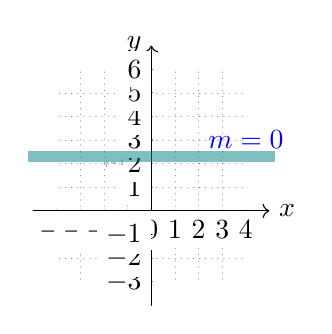
\begin{tikzpicture}[scale=0.3,cap=round]

% Styles
\tikzstyle{axes}=[]
\tikzstyle help lines=[color=blue!50,very thin,dotted]


%%%%%%%%%%%%%%%%%%%%%%%%%%%%%%%%
%		GRID
%%%%%%%%%%%%%%%%%%%%%%%%%%%%%%%%

\draw[style=help lines,step=1cm] (-3.9,-2.9) grid (3.9,5.9);



%%%%%%%%%%%%%%%%%%%%%%%%%%%%%%%%
%		ASSENSTELSEL
%%%%%%%%%%%%%%%%%%%%%%%%%%%%%%%%

\draw[->] (-5,0) -- (5,0) node[right] {$x$};
\draw[->] (0,-4) -- (0,7) node[left]{$y$};

%\draw[fill,cyan](1,1)circle [radius=0.025];

%\draw[red,cap=rect, loosely dashed, ultra thick, domain=-2:2] plot (\x, {(\x*\x-1)+0.05}) node[above,yshift=-.7cm, right]{};

%%%%%%%%%%%%%%%%%%%%%%%%%%%%%%%%
%legende
%%%%%%%%%%%%%%%%%%%%%%%%%%%%%%%%
%\tkzDefPoint(0.5,3.5){A}
%\tkzDefPoint(1,3.5){B}
%\tkzLabelPoint[right,xshift=+0.1cm](B){${\color{cyan}f(x)=|x^2-1|}$}
%\tkzDrawSegment[cyan,ultra thick](A,B)

%\tkzDefPoint(0.5,3.2){C}
%\tkzDefPoint(1,3.2){D}
%\tkzLabelPoint[right,xshift=+0.1cm](D){${\color{red}e(x)=x^2-1}$}
%\tkzDrawSegment[red,cap=rect, loosely dashed, ultra thick](C,D)


%%%%%%%%%%%%%%%%%%%%%%%%%%%%%%%%
%getallen op de x-as en lijntjes
%%%%%%%%%%%%%%%%%%%%%%%%%%%%%%%%   
\foreach \x/\xtext in {-4,-3,-2,-1,0,1,2,3,4}
	\draw[xshift=\x cm] (0pt,1pt) -- (0pt,0pt) node[below,fill=white]
	{$\xtext$};,3
	
%getallen op de y-as en lijntjes  
%BEGIN LUS
\foreach \y/\ytext in {-3,-2,-1,1,2,3,4,5,6}
	\draw[yshift=\y cm] (1pt,0pt) -- (0pt,0pt) node[left,fill=white]
	{$\ytext$}; %EINDE LUS



%%%%%%%%%%%%%%%%%%%%%%%%%%%%%%%%
%		GRAFIEKEN
%%%%%%%%%%%%%%%%%%%%%%%%%%%%%%%%
%\draw[cyan,cap=rect,thick, domain=-6:6] plot (\x, \x) node[above, right]{${\color{cyan}y=x}$};


\draw[teal,cap=rect,line width=4, opacity=.5, domain=-5:5] plot (\x, {
	2.3 		% <- plaats het functievoorschrift hier
}) node[opacity=1,left,pos=1,xshift=-1cm, yshift=+2cm]{$q=3$};
 
%node[blue]{stijgen} 
%\draw[cyan,cap=rect,ultra thick, domain=2.25:6] plot (\x, {(\x-2)^(-1)}) node[above,yshift=+0.5cm,left]{$\color{cyan} y=\frac{1}{x-2}$};


%\draw[cyan,cap=rect,ultra thick, domain=-7:1.9] plot (\x, {exp{\x}}) node[above, right]{${\color{cyan}y=\exp{x}}$};

%%%%%%%%%%%%%%%%%%%%%%%%%%%%%%%%
%		MARKERINGEN
%%%%%%%%%%%%%%%%%%%%%%%%%%%%%%%%
%verticale lijn
%\draw[-o,line width=4,teal, cap=rect,opacity=0.3] (0,-4) -- (0,0.25) node[right] {};
%\draw[line width=4,teal, cap=rect,opacity=0.3] (0,0) -- (0,4.2) node[right] {bld $f$ = $\mathbb{R}_0$};
%horizontale lijn

%horizontale lijn





% \draw[white,fill=blue,opacity=.5] (1,-2) circle [radius=.1]   node[blue, above,xshift=-1.1cm,opacity=1] {buigpunt in $(1,-2)$};

\draw[] (2,3) node[blue,right] {$m=0$};



\end{tikzpicture}
  &  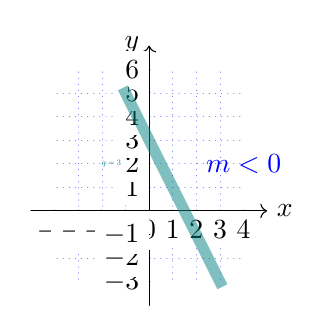
\begin{tikzpicture}[scale=0.3,cap=round]

% Styles
\tikzstyle{axes}=[]
\tikzstyle help lines=[color=blue!50,very thin,dotted]


%%%%%%%%%%%%%%%%%%%%%%%%%%%%%%%%
%		GRID
%%%%%%%%%%%%%%%%%%%%%%%%%%%%%%%%

\draw[style=help lines,step=1cm] (-3.9,-2.9) grid (3.9,5.9);



%%%%%%%%%%%%%%%%%%%%%%%%%%%%%%%%
%		ASSENSTELSEL
%%%%%%%%%%%%%%%%%%%%%%%%%%%%%%%%

\draw[->] (-5,0) -- (5,0) node[right] {$x$};
\draw[->] (0,-4) -- (0,7) node[left]{$y$};

%\draw[fill,cyan](1,1)circle [radius=0.025];

%\draw[red,cap=rect, loosely dashed, ultra thick, domain=-2:2] plot (\x, {(\x*\x-1)+0.05}) node[above,yshift=-.7cm, right]{};

%%%%%%%%%%%%%%%%%%%%%%%%%%%%%%%%
%legende
%%%%%%%%%%%%%%%%%%%%%%%%%%%%%%%%
%\tkzDefPoint(0.5,3.5){A}
%\tkzDefPoint(1,3.5){B}
%\tkzLabelPoint[right,xshift=+0.1cm](B){${\color{cyan}f(x)=|x^2-1|}$}
%\tkzDrawSegment[cyan,ultra thick](A,B)

%\tkzDefPoint(0.5,3.2){C}
%\tkzDefPoint(1,3.2){D}
%\tkzLabelPoint[right,xshift=+0.1cm](D){${\color{red}e(x)=x^2-1}$}
%\tkzDrawSegment[red,cap=rect, loosely dashed, ultra thick](C,D)


%%%%%%%%%%%%%%%%%%%%%%%%%%%%%%%%
%getallen op de x-as en lijntjes
%%%%%%%%%%%%%%%%%%%%%%%%%%%%%%%%   
\foreach \x/\xtext in {-4,-3,-2,-1,0,1,2,3,4}
	\draw[xshift=\x cm] (0pt,1pt) -- (0pt,0pt) node[below,fill=white]
	{$\xtext$};,3
	
%getallen op de y-as en lijntjes  
%BEGIN LUS
\foreach \y/\ytext in {-3,-2,-1,1,2,3,4,5,6}
	\draw[yshift=\y cm] (1pt,0pt) -- (0pt,0pt) node[left,fill=white]
	{$\ytext$}; %EINDE LUS



%%%%%%%%%%%%%%%%%%%%%%%%%%%%%%%%
%		GRAFIEKEN
%%%%%%%%%%%%%%%%%%%%%%%%%%%%%%%%
%\draw[cyan,cap=rect,thick, domain=-6:6] plot (\x, \x) node[above, right]{${\color{cyan}y=x}$};


\draw[teal,cap=rect,line width=4, opacity=.5, domain=-1:3] plot (\x, {
	(-2)*\x + 3  		% <- plaats het functievoorschrift hier
}) node[opacity=1,left,pos=1,xshift=-1cm, yshift=+2cm]{$q=3$};
 
%node[blue]{stijgen} 
%\draw[cyan,cap=rect,ultra thick, domain=2.25:6] plot (\x, {(\x-2)^(-1)}) node[above,yshift=+0.5cm,left]{$\color{cyan} y=\frac{1}{x-2}$};


%\draw[cyan,cap=rect,ultra thick, domain=-7:1.9] plot (\x, {exp{\x}}) node[above, right]{${\color{cyan}y=\exp{x}}$};

%%%%%%%%%%%%%%%%%%%%%%%%%%%%%%%%
%		MARKERINGEN
%%%%%%%%%%%%%%%%%%%%%%%%%%%%%%%%
%verticale lijn
%\draw[-o,line width=4,teal, cap=rect,opacity=0.3] (0,-4) -- (0,0.25) node[right] {};
%\draw[line width=4,teal, cap=rect,opacity=0.3] (0,0) -- (0,4.2) node[right] {bld $f$ = $\mathbb{R}_0$};
%horizontale lijn

%horizontale lijn




% \draw[white,fill=blue,opacity=.5] (1,-2) circle [radius=.1]   node[blue, above,xshift=-1.1cm,opacity=1] {buigpunt in $(1,-2)$};

\draw[] (2,2) node[blue,right] {$m<0$};



\end{tikzpicture}
   \\
%\hline
\end{tabular}

\tikzsetfigurename{Fig_module_2_1_2_reele_functies_vb1}
%TODO polynoombenadering uitrekenen > zie cursus Algebra

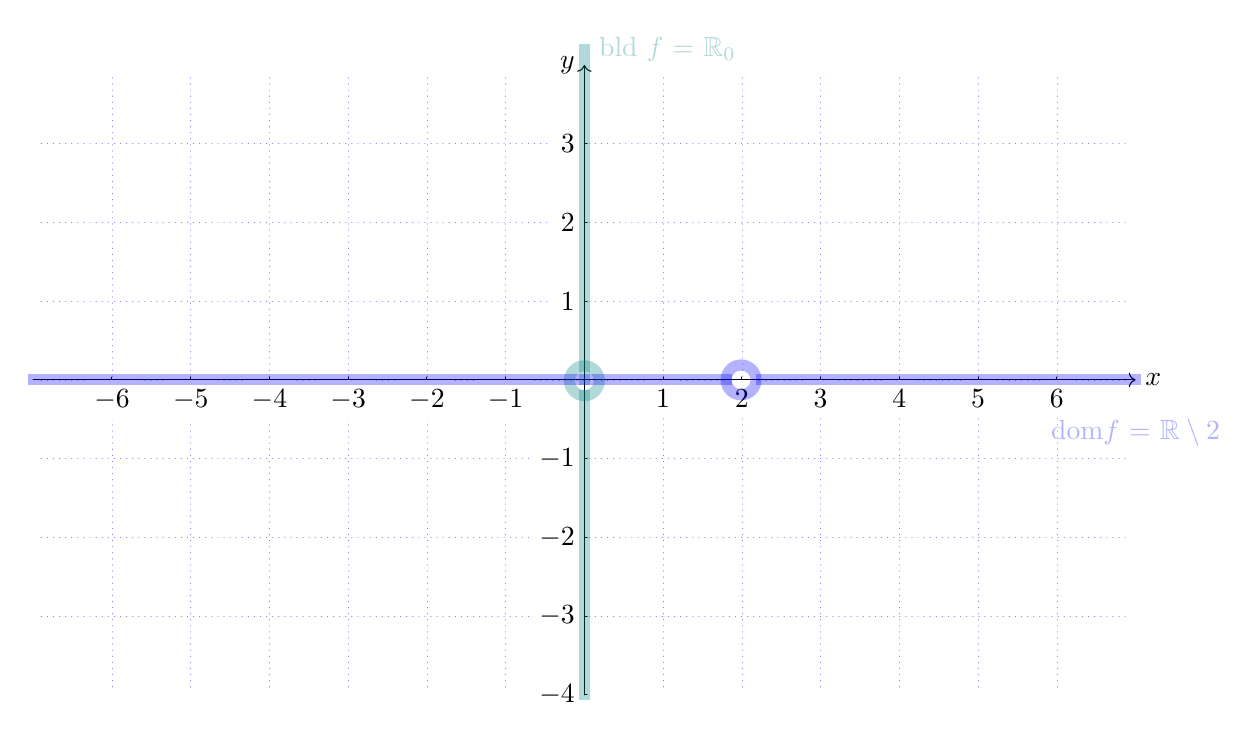
\begin{tikzpicture}[cap=round]

% Styles
\tikzstyle{axes}=[]
\tikzstyle help lines=[color=blue!50,very thin,dotted]


%%%%%%%%%%%%%%%%%%%%%%%%%%%%%%%%
%		GRID
%%%%%%%%%%%%%%%%%%%%%%%%%%%%%%%%

\draw[style=help lines,step=1cm] (-6.9,-3.9) grid (6.9,3.9);



%%%%%%%%%%%%%%%%%%%%%%%%%%%%%%%%
%		ASSENSTELSEL
%%%%%%%%%%%%%%%%%%%%%%%%%%%%%%%%

\draw[->] (-7,0) -- (7,0) node[right] {$x$};
\draw[->] (0,-4) -- (0,4) node[left]{$y$};

%\draw[fill,cyan](1,1)circle [radius=0.025];

%\draw[red,cap=rect, loosely dashed, ultra thick, domain=-2:2] plot (\x, {(\x*\x-1)+0.05}) node[above,yshift=-.7cm, right]{};

%%%%%%%%%%%%%%%%%%%%%%%%%%%%%%%%
%legende
%%%%%%%%%%%%%%%%%%%%%%%%%%%%%%%%
%\tkzDefPoint(0.5,3.5){A}
%\tkzDefPoint(1,3.5){B}
%\tkzLabelPoint[right,xshift=+0.1cm](B){${\color{cyan}f(x)=|x^2-1|}$}
%\tkzDrawSegment[cyan,ultra thick](A,B)

%\tkzDefPoint(0.5,3.2){C}
%\tkzDefPoint(1,3.2){D}
%\tkzLabelPoint[right,xshift=+0.1cm](D){${\color{red}e(x)=x^2-1}$}
%\tkzDrawSegment[red,cap=rect, loosely dashed, ultra thick](C,D)


%%%%%%%%%%%%%%%%%%%%%%%%%%%%%%%%
%getallen op de x-as en lijntjes
%%%%%%%%%%%%%%%%%%%%%%%%%%%%%%%%   
\foreach \x/\xtext in {-6,-5,-4,-3,-2,-1,1,2,3,4,5,6}
	\draw[xshift=\x cm] (0pt,1pt) -- (0pt,0pt) node[below,fill=white]
	{$\xtext$};,3
	
%getallen op de y-as en lijntjes  
%BEGIN LUS
\foreach \y/\ytext in {-4,-3,-2,-1,1,2,3}
	\draw[yshift=\y cm] (1pt,0pt) -- (0pt,0pt) node[left,fill=white]
	{$\ytext$}; %EINDE LUS



%%%%%%%%%%%%%%%%%%%%%%%%%%%%%%%%
%		GRAFIEKEN
%%%%%%%%%%%%%%%%%%%%%%%%%%%%%%%%
%\draw[cyan,cap=rect,thick, domain=-6:6] plot (\x, \x) node[above, right]{${\color{cyan}y=x}$};v

%\draw[cyan,cap=rect,ultra thick, domain=-6:1.75] plot (\x, {(\x-2)^(-1)}) node[above,right]{};


%\draw[cyan,cap=rect,ultra thick, domain=2.25:6] plot (\x, {(\x-2)^(-1)}) node[above,yshift=+0.5cm,left]{$\color{cyan} y=\frac{1}{x-2}$};


%\draw[cyan,cap=rect,ultra thick, domain=-7:1.9] plot (\x, {exp{\x}}) node[above, right]{${\color{cyan}y=\exp{x}}$};

%%%%%%%%%%%%%%%%%%%%%%%%%%%%%%%%
%		MARKERINGEN
%%%%%%%%%%%%%%%%%%%%%%%%%%%%%%%%
%verticale lijn
\draw[-o,line width=4,teal, cap=rect,opacity=0.3] (0,-4) -- (0,0.25) node[right] {};
\draw[line width=4,teal, cap=rect,opacity=0.3] (0,0) -- (0,4.2) node[right] {bld $f$ = $\mathbb{R}_0$};
%horizontale lijn
\draw[arrows=-o,line width=4,blue, cap=rect,opacity=0.3] (-7,0) -- (2.25,0) node[right] {};
\draw[line width=4,blue, cap=rect,opacity=0.3] (2.25,0) -- (7,0) node[below,yshift=-0.3cm] {dom$f$ = $\mathbb{R}  \setminus 2 $};
 
\end{tikzpicture}


%
\begin{center}
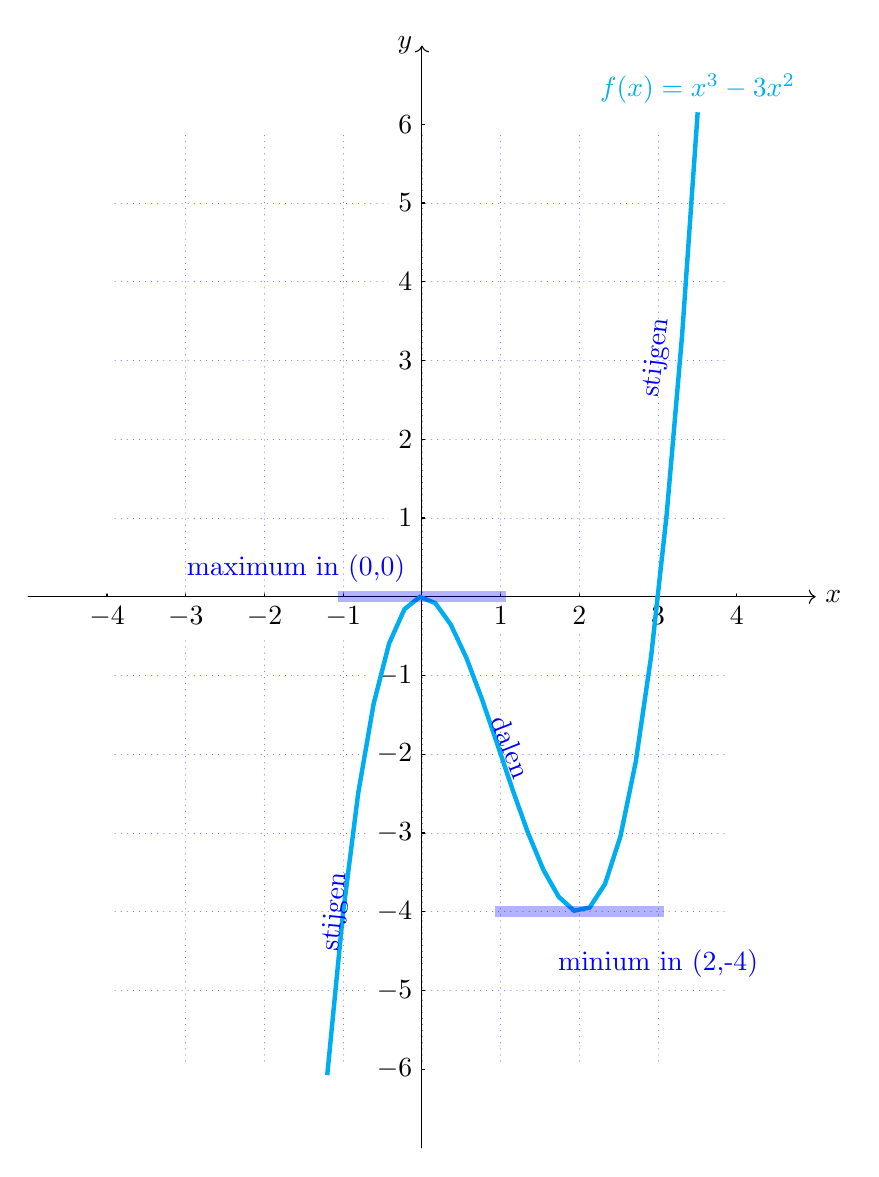
\begin{tikzpicture}[scale=1,cap=round]

% Styles
\tikzstyle{axes}=[]
\tikzstyle help lines=[color=blue!50,very thin,dotted]


%%%%%%%%%%%%%%%%%%%%%%%%%%%%%%%%
%		GRID
%%%%%%%%%%%%%%%%%%%%%%%%%%%%%%%%

\draw[style=help lines,step=1cm] (-3.9,-5.9) grid (3.9,5.9);



%%%%%%%%%%%%%%%%%%%%%%%%%%%%%%%%
%		ASSENSTELSEL
%%%%%%%%%%%%%%%%%%%%%%%%%%%%%%%%

\draw[->] (-5,0) -- (5,0) node[right] {$x$};
\draw[->] (0,-7) -- (0,7) node[left]{$y$};

%\draw[fill,cyan](1,1)circle [radius=0.025];

%\draw[red,cap=rect, loosely dashed, ultra thick, domain=-2:2] plot (\x, {(\x*\x-1)+0.05}) node[above,yshift=-.7cm, right]{};

%%%%%%%%%%%%%%%%%%%%%%%%%%%%%%%%
%legende
%%%%%%%%%%%%%%%%%%%%%%%%%%%%%%%%
%\tkzDefPoint(0.5,3.5){A}
%\tkzDefPoint(1,3.5){B}
%\tkzLabelPoint[right,xshift=+0.1cm](B){${\color{cyan}f(x)=|x^2-1|}$}
%\tkzDrawSegment[cyan,ultra thick](A,B)

%\tkzDefPoint(0.5,3.2){C}
%\tkzDefPoint(1,3.2){D}
%\tkzLabelPoint[right,xshift=+0.1cm](D){${\color{red}e(x)=x^2-1}$}
%\tkzDrawSegment[red,cap=rect, loosely dashed, ultra thick](C,D)


%%%%%%%%%%%%%%%%%%%%%%%%%%%%%%%%
%getallen op de x-as en lijntjes
%%%%%%%%%%%%%%%%%%%%%%%%%%%%%%%%   
\foreach \x/\xtext in {-4,-3,-2,-1,1,2,3,4}
	\draw[xshift=\x cm] (0pt,1pt) -- (0pt,0pt) node[below,fill=white]
	{$\xtext$};,3
	
%getallen op de y-as en lijntjes  
%BEGIN LUS
\foreach \y/\ytext in {-6,-5,-4,-3,-2,-1,1,2,3,4,5,6}
	\draw[yshift=\y cm] (1pt,0pt) -- (0pt,0pt) node[left,fill=white]
	{$\ytext$}; %EINDE LUS



%%%%%%%%%%%%%%%%%%%%%%%%%%%%%%%%
%		GRAFIEKEN
%%%%%%%%%%%%%%%%%%%%%%%%%%%%%%%%
%\draw[cyan,cap=rect,thick, domain=-6:6] plot (\x, \x) node[above, right]{${\color{cyan}y=x}$};

\draw[cyan,cap=rect,ultra thick, domain=-1.2:3.5] plot (\x, {
	pow(\x,3)-3*pow(\x,2)		% <- plaats het functievoorschrift hier
}) node[above]{$f(x)=x^3-3x^2$};

\draw[opacity=0] (-1.2,-5) --(-1,-3) node[opacity=1,blue, midway,sloped]{stijgen};  
\draw[opacity=0] (0.5,-1) --(1.3,-3) node[opacity=1,blue, midway,sloped,above]{dalen};  
\draw[opacity=0] (3,1) --(3.5,5) node[opacity=1,blue, midway,sloped,above]{stijgen};  


%node[blue]{stijgen} 
%\draw[cyan,cap=rect,ultra thick, domain=2.25:6] plot (\x, {(\x-2)^(-1)}) node[above,yshift=+0.5cm,left]{$\color{cyan} y=\frac{1}{x-2}$};


%\draw[cyan,cap=rect,ultra thick, domain=-7:1.9] plot (\x, {exp{\x}}) node[above, right]{${\color{cyan}y=\exp{x}}$};

%%%%%%%%%%%%%%%%%%%%%%%%%%%%%%%%
%		MARKERINGEN
%%%%%%%%%%%%%%%%%%%%%%%%%%%%%%%%
%verticale lijn
%\draw[-o,line width=4,teal, cap=rect,opacity=0.3] (0,-4) -- (0,0.25) node[right] {};
%\draw[line width=4,teal, cap=rect,opacity=0.3] (0,0) -- (0,4.2) node[right] {bld $f$ = $\mathbb{R}_0$};
%horizontale lijn
\draw[line width=4,blue, cap=rect,opacity=0.3] (-1,0) -- (1,0) node[near start,above,xshift=-1.1cm,opacity=1] {maximum in (0,0)};

 
\draw[line width=4,blue, cap=rect,opacity=0.3] (1,-4) -- (3,-4) node[below,yshift=-.3cm,opacity=1] {minium in (2,-4)};
\end{tikzpicture}
\end{center}

%
\begin{center}
\begin{tikzpicture}[scale=1,cap=round]

% Styles
\tikzstyle{axes}=[]
\tikzstyle help lines=[color=blue!50,very thin,dotted]


%%%%%%%%%%%%%%%%%%%%%%%%%%%%%%%%
%		GRID
%%%%%%%%%%%%%%%%%%%%%%%%%%%%%%%%

\draw[style=help lines,step=1cm] (-3.9,-5.9) grid (3.9,5.9);



%%%%%%%%%%%%%%%%%%%%%%%%%%%%%%%%
%		ASSENSTELSEL
%%%%%%%%%%%%%%%%%%%%%%%%%%%%%%%%

\draw[->] (-5,0) -- (7,0) node[right] {$x$};
\draw[->] (0,-7) -- (0,7) node[left]{$y$};

%\draw[fill,cyan](1,1)circle [radius=0.025];

%\draw[red,cap=rect, loosely dashed, ultra thick, domain=-2:2] plot (\x, {(\x*\x-1)+0.05}) node[above,yshift=-.7cm, right]{};

%%%%%%%%%%%%%%%%%%%%%%%%%%%%%%%%
%legende
%%%%%%%%%%%%%%%%%%%%%%%%%%%%%%%%
%\tkzDefPoint(0.5,3.5){A}
%\tkzDefPoint(1,3.5){B}
%\tkzLabelPoint[right,xshift=+0.1cm](B){${\color{cyan}f(x)=|x^2-1|}$}
%\tkzDrawSegment[cyan,ultra thick](A,B)

%\tkzDefPoint(0.5,3.2){C}
%\tkzDefPoint(1,3.2){D}
%\tkzLabelPoint[right,xshift=+0.1cm](D){${\color{red}e(x)=x^2-1}$}
%\tkzDrawSegment[red,cap=rect, loosely dashed, ultra thick](C,D)


%%%%%%%%%%%%%%%%%%%%%%%%%%%%%%%%
%getallen op de x-as en lijntjes
%%%%%%%%%%%%%%%%%%%%%%%%%%%%%%%%   
\foreach \x/\xtext in {-4,-3,-2,-1,1,2,3,4}
	\draw[xshift=\x cm] (0pt,1pt) -- (0pt,0pt) node[below,fill=white]
	{$\xtext$};,3
	
%getallen op de y-as en lijntjes  
%BEGIN LUS
\foreach \y/\ytext in {-6,-5,-4,-3,-2,-1,1,2,3,4,5,6}
	\draw[yshift=\y cm] (1pt,0pt) -- (0pt,0pt) node[left,fill=white]
	{$\ytext$}; %EINDE LUS



%%%%%%%%%%%%%%%%%%%%%%%%%%%%%%%%
%		GRAFIEKEN
%%%%%%%%%%%%%%%%%%%%%%%%%%%%%%%%
%\draw[cyan,cap=rect,thick, domain=-6:6] plot (\x, \x) node[above, right]{${\color{cyan}y=x}$};

\draw[cyan,cap=rect,ultra thick, domain=-1.2:3.5] plot (\x, {
	pow(\x,3)-3*pow(\x,2)		% <- plaats het functievoorschrift hier
}) node[above]{$f(x)=x^3-3x^2$};

 
%node[blue]{stijgen} 
%\draw[cyan,cap=rect,ultra thick, domain=2.25:6] plot (\x, {(\x-2)^(-1)}) node[above,yshift=+0.5cm,left]{$\color{cyan} y=\frac{1}{x-2}$};


%\draw[cyan,cap=rect,ultra thick, domain=-7:1.9] plot (\x, {exp{\x}}) node[above, right]{${\color{cyan}y=\exp{x}}$};

%%%%%%%%%%%%%%%%%%%%%%%%%%%%%%%%
%		MARKERINGEN
%%%%%%%%%%%%%%%%%%%%%%%%%%%%%%%%
%verticale lijn
%\draw[-o,line width=4,teal, cap=rect,opacity=0.3] (0,-4) -- (0,0.25) node[right] {};
%\draw[line width=4,teal, cap=rect,opacity=0.3] (0,0) -- (0,4.2) node[right] {bld $f$ = $\mathbb{R}_0$};
%horizontale lijn

 \draw[white,fill=blue,opacity=.5] (1,-2) circle [radius=.1]   node[blue, above,xshift=-1.1cm,opacity=1] {buigpunt in $(1,-2)$};


 
\draw[teal,cap=rect,line width=4, opacity=.5, domain=.5:1.5] plot (\x, {
	-2-3*(\x-1)		% <- plaats het functievoorschrift hier
}) node[opacity=1,above]{};


\draw[] (1.5,1.5) node[blue] {hol of concaaf};
\draw[] (1.5,-5) node[blue] {bol of convex};

\end{tikzpicture}
\end{center}


%\tikzsetfigurename{Fig_module_2_1_3_verloop_stijgen_dalen}

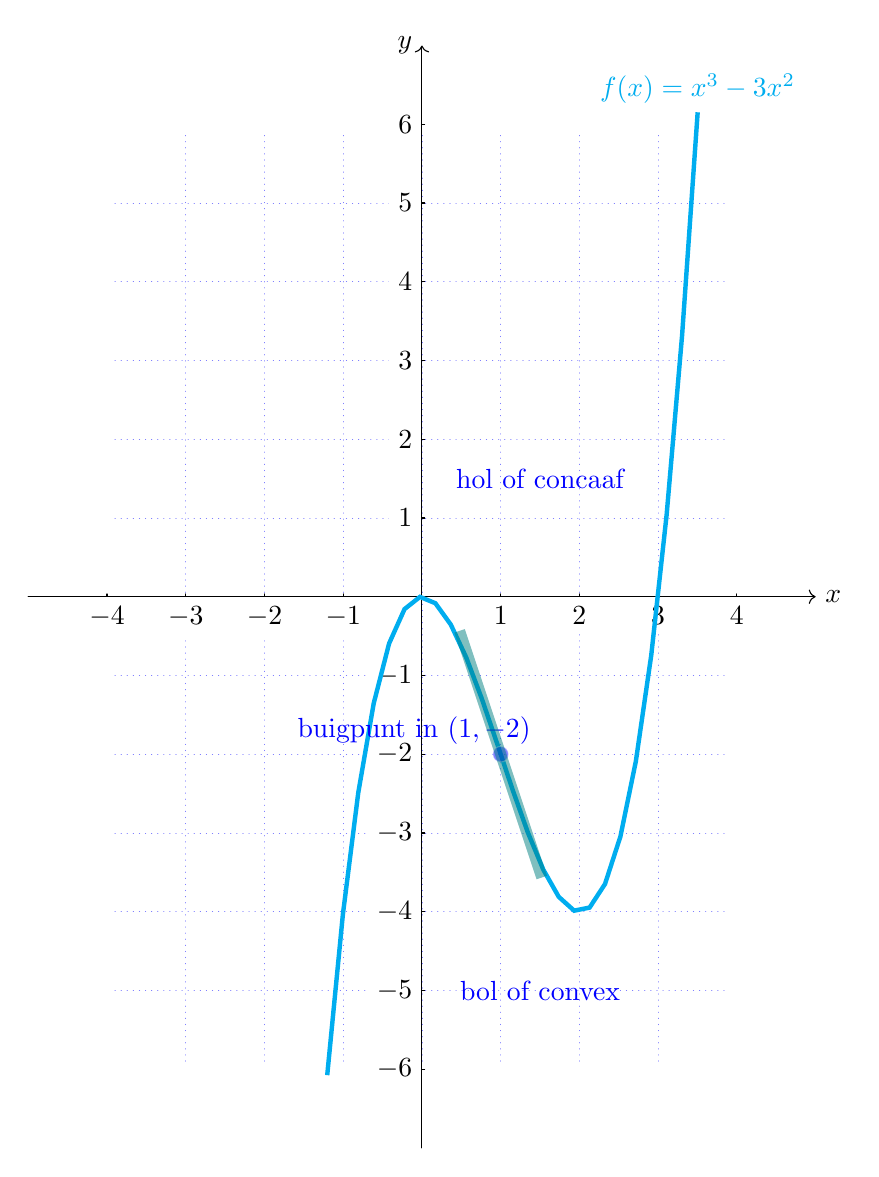
\begin{tikzpicture}[scale=1,cap=round]

% Styles
\tikzstyle{axes}=[]
\tikzstyle help lines=[color=blue!50,very thin,dotted]


%%%%%%%%%%%%%%%%%%%%%%%%%%%%%%%%
%		GRID
%%%%%%%%%%%%%%%%%%%%%%%%%%%%%%%%

\draw[style=help lines,step=1cm] (-3.9,-5.9) grid (3.9,5.9);



%%%%%%%%%%%%%%%%%%%%%%%%%%%%%%%%
%		ASSENSTELSEL
%%%%%%%%%%%%%%%%%%%%%%%%%%%%%%%%

\draw[->] (-5,0) -- (5,0) node[right] {$x$};
\draw[->] (0,-7) -- (0,7) node[left]{$y$};

%\draw[fill,cyan](1,1)circle [radius=0.025];

%\draw[red,cap=rect, loosely dashed, ultra thick, domain=-2:2] plot (\x, {(\x*\x-1)+0.05}) node[above,yshift=-.7cm, right]{};

%%%%%%%%%%%%%%%%%%%%%%%%%%%%%%%%
%legende
%%%%%%%%%%%%%%%%%%%%%%%%%%%%%%%%
%\tkzDefPoint(0.5,3.5){A}
%\tkzDefPoint(1,3.5){B}
%\tkzLabelPoint[right,xshift=+0.1cm](B){${\color{cyan}f(x)=|x^2-1|}$}
%\tkzDrawSegment[cyan,ultra thick](A,B)

%\tkzDefPoint(0.5,3.2){C}
%\tkzDefPoint(1,3.2){D}
%\tkzLabelPoint[right,xshift=+0.1cm](D){${\color{red}e(x)=x^2-1}$}
%\tkzDrawSegment[red,cap=rect, loosely dashed, ultra thick](C,D)


%%%%%%%%%%%%%%%%%%%%%%%%%%%%%%%%
%getallen op de x-as en lijntjes
%%%%%%%%%%%%%%%%%%%%%%%%%%%%%%%%   
\foreach \x/\xtext in {-4,-3,-2,-1,1,2,3,4}
	\draw[xshift=\x cm] (0pt,1pt) -- (0pt,0pt) node[below,fill=white]
	{$\xtext$};,3
	
%getallen op de y-as en lijntjes  
%BEGIN LUS
\foreach \y/\ytext in {-6,-5,-4,-3,-2,-1,1,2,3,4,5,6}
	\draw[yshift=\y cm] (1pt,0pt) -- (0pt,0pt) node[left,fill=white]
	{$\ytext$}; %EINDE LUS



%%%%%%%%%%%%%%%%%%%%%%%%%%%%%%%%
%		GRAFIEKEN
%%%%%%%%%%%%%%%%%%%%%%%%%%%%%%%%
%\draw[cyan,cap=rect,thick, domain=-6:6] plot (\x, \x) node[above, right]{${\color{cyan}y=x}$};

\draw[cyan,cap=rect,ultra thick, domain=-1.2:3.5] plot (\x, {
	pow(\x,3)-3*pow(\x,2)		% <- plaats het functievoorschrift hier
}) node[above]{$f(x)=x^3-3x^2$};

 
%node[blue]{stijgen} 
%\draw[cyan,cap=rect,ultra thick, domain=2.25:6] plot (\x, {(\x-2)^(-1)}) node[above,yshift=+0.5cm,left]{$\color{cyan} y=\frac{1}{x-2}$};


%\draw[cyan,cap=rect,ultra thick, domain=-7:1.9] plot (\x, {exp{\x}}) node[above, right]{${\color{cyan}y=\exp{x}}$};

%%%%%%%%%%%%%%%%%%%%%%%%%%%%%%%%
%		MARKERINGEN
%%%%%%%%%%%%%%%%%%%%%%%%%%%%%%%%
%verticale lijn
%\draw[-o,line width=4,teal, cap=rect,opacity=0.3] (0,-4) -- (0,0.25) node[right] {};
%\draw[line width=4,teal, cap=rect,opacity=0.3] (0,0) -- (0,4.2) node[right] {bld $f$ = $\mathbb{R}_0$};
%horizontale lijn

 \draw[white,fill=blue,opacity=.5] (1,-2) circle [radius=.1]   node[blue, above,xshift=-1.1cm,opacity=1] {buigpunt in $(1,-2)$};


 
\draw[teal,cap=rect,line width=4, opacity=.5, domain=.5:1.5] plot (\x, {
	-2-3*(\x-1)		% <- plaats het functievoorschrift hier
}) node[opacity=1,above]{};


\draw[] (1.5,1.5) node[blue] {hol of concaaf};
\draw[] (1.5,-5) node[blue] {bol of convex};

\end{tikzpicture}
 
%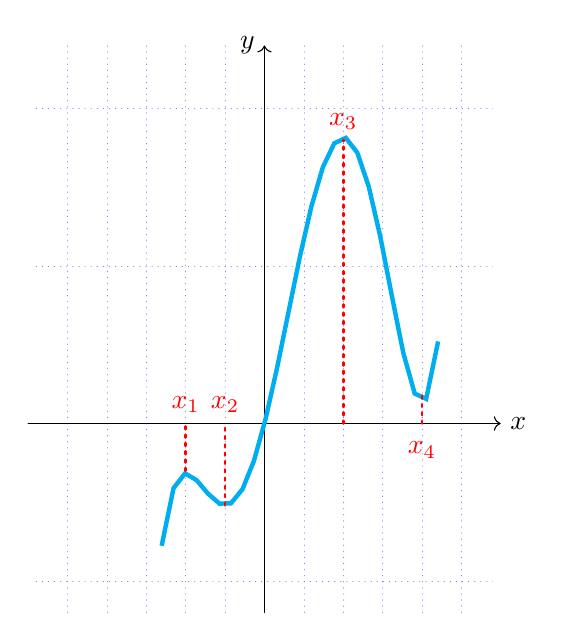
\begin{tikzpicture}[xscale=1,yscale=4,cap=round]

% Styles
\tikzstyle{axes}=[]
\tikzstyle help lines=[color=blue!50,very thin,dotted]

%%%%%%%%%%%%%%%%%%%%%%%%%%%%%%%%
%		GRID
%%%%%%%%%%%%%%%%%%%%%%%%%%%%%%%%

\draw[style=help lines,step=0.5cm] (-2.9,-0.6) grid (2.9,1.2);

%%%%%%%%%%%%%%%%%%%%%%%%%%%%%%%%
%		ASSENSTELSEL
%%%%%%%%%%%%%%%%%%%%%%%%%%%%%%%%

\draw[->] (-3,0) -- (3,0) node[right] {$x$};
\draw[->] (0,-0.6) -- (0,1.2) node[left]{$y$};

%\draw[fill,cyan](1,1)circle [radius=0.025];
%\draw[red,cap=rect, loosely dashed, ultra thick, domain=-2:2] plot (\x, {(\x*\x-1)+0.05}) node[above,yshift=-.7cm, right]{};

%%%%%%%%%%%%%%%%%%%%%%%%%%%%%%%%
%legende
%%%%%%%%%%%%%%%%%%%%%%%%%%%%%%%%
%\tkzDefPoint(0.5,3.5){A}
%\tkzDefPoint(1,3.5){B}
%\tkzLabelPoint[right,xshift=+0.1cm](B){${\color{cyan}f(x)=|x^2-1|}$}
%\tkzDrawSegment[cyan,ultra thick](A,B)

%\tkzDefPoint(0.5,3.2){C}
%\tkzDefPoint(1,3.2){D}
%\tkzLabelPoint[right,xshift=+0.1cm](D){${\color{red}e(x)=x^2-1}$}
%\tkzDrawSegment[red,cap=rect, loosely dashed, ultra thick](C,D)


%%%%%%%%%%%%%%%%%%%%%%%%%%%%%%%%
%getallen op de x-as en lijntjes
%%%%%%%%%%%%%%%%%%%%%%%%%%%%%%%%   
%\foreach \x/\xtext in {-2,-1,1,2}
%	\draw[xshift=\x cm] (0pt,1pt) -- (0pt,0pt) node[below,fill=white]
%	{$\xtext$};,3
	
%getallen op de y-as en lijntjes  
%BEGIN LUS
%\foreach \y/\ytext in {-1,1}
%	\draw[yshift=\y cm] (1pt,0pt) -- (0pt,0pt) node[left,fill=white]
%	{$\ytext$}; %EINDE LUS



%%%%%%%%%%%%%%%%%%%%%%%%%%%%%%%%
%		GRAFIEKEN
%%%%%%%%%%%%%%%%%%%%%%%%%%%%%%%%
%1.926583164702752926
%0.6148052613028164304
%%-14.35341068538563647
%-59.14215224350418509
%104.9541745028843565
%191

\draw[cyan,cap=rect,ultra thick, domain=-1.3:2.2] plot (\x, {
0.2*pow(\x,5)-(3/8)*pow(\x,4)-(2/3)*pow(\x,3)+(3/4)*pow(\x,2)+\x 	
%	*(	(\x+2)*(\x+1)*(\x+0.5)*(\x-1)*(\x-2) ) *0.2
	%pow(\x,5)+0.5*pow(\x,4)-5*pow(\x,3)+3*pow(\x,1)-1 )*.1 
	% <- plaats het functievoorschrift hier
}) node[above, yshift=+0.5cm,xshift=+1.3cm]{$$};
%f(x)=x^5+\frac{1}{2}x^4-5x^3-\frac{5}{2}x^2+4x-2

 
%node[blue]{stijgen} 
%\draw[cyan,cap=rect,ultra thick, domain=2.25:6] plot (\x, {(\x-2)^(-1)}) node[above,yshift=+0.5cm,left]{$\color{cyan} y=\frac{1}{x-2}$};


%\draw[cyan,cap=rect,ultra thick, domain=-7:1.9] plot (\x, {exp{\x}}) node[above, right]{${\color{cyan}y=\exp{x}}$};

%%%%%%%%%%%%%%%%%%%%%%%%%%%%%%%%
%		MARKERINGEN
%%%%%%%%%%%%%%%%%%%%%%%%%%%%%%%%
%verticale lijn
\draw[line width=1,red, dotted, opacity=1] (-1,-.15) -- (-1,0) node[above] {$x_1$};
\draw[line width=1,red, dotted, opacity=1] (-0.5,-.26) -- (-0.5,0) node[above] {$x_2$};
\draw[line width=1,red,opacity=1,dotted] (1,0) -- (1,0.9) node[above] {$x_3$};
\draw[line width=1,red,opacity=1,dotted] (2,0) -- (2,0.1) node[below,yshift=-.5cm] {$x_4$};
%\draw[line width=4,teal, cap=rect,opacity=0.3] (0,0) -- (0,4.2) node[right] {bld $f$ = $\mathbb{R}_0$};
%horizontale lijn

% \draw[white,fill=blue,opacity=.5] (1,-2) circle [radius=.1]   node[blue, above,xshift=-1.1cm,opacity=1] {buigpunt in $(1,-2)$};


 
%\draw[teal,cap=rect,line width=4, opacity=.5, domain=.5:1.5] plot (\x, {
%	-2-3*(\x-1)		% <- plaats het functievoorschrift hier
%}) node[opacity=1,above]{};


%\draw[] (1.5,1.5) node[blue] {hol of concaaf};
%\draw[] (1.5,-5) node[blue] {bol of convex};

\end{tikzpicture}
 
%
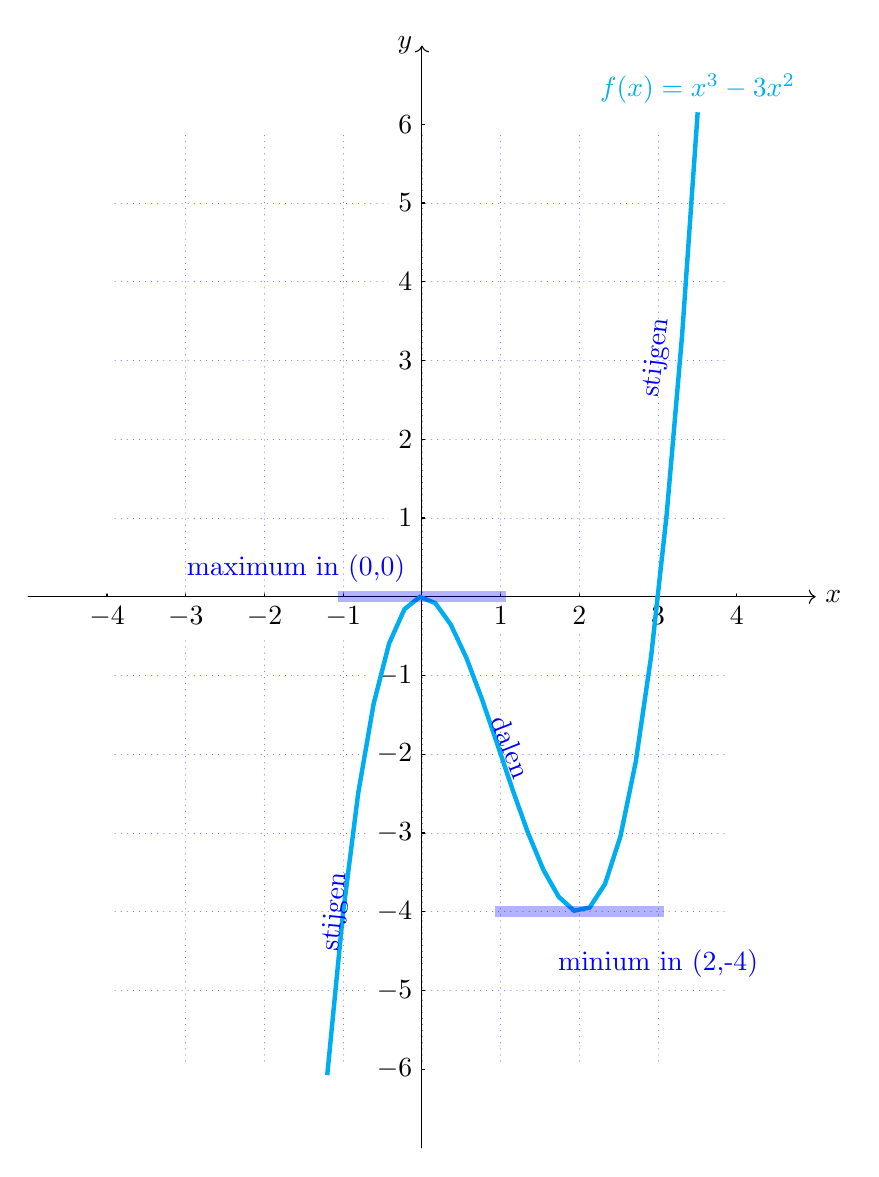
\begin{tikzpicture}[scale=1,cap=round]

% Styles
\tikzstyle{axes}=[]
\tikzstyle help lines=[color=blue!50,very thin,dotted]


%%%%%%%%%%%%%%%%%%%%%%%%%%%%%%%%
%		GRID
%%%%%%%%%%%%%%%%%%%%%%%%%%%%%%%%

\draw[style=help lines,step=1cm] (-3.9,-5.9) grid (3.9,5.9);



%%%%%%%%%%%%%%%%%%%%%%%%%%%%%%%%
%		ASSENSTELSEL
%%%%%%%%%%%%%%%%%%%%%%%%%%%%%%%%

\draw[->] (-5,0) -- (5,0) node[right] {$x$};
\draw[->] (0,-7) -- (0,7) node[left]{$y$};

%\draw[fill,cyan](1,1)circle [radius=0.025];

%\draw[red,cap=rect, loosely dashed, ultra thick, domain=-2:2] plot (\x, {(\x*\x-1)+0.05}) node[above,yshift=-.7cm, right]{};

%%%%%%%%%%%%%%%%%%%%%%%%%%%%%%%%
%legende
%%%%%%%%%%%%%%%%%%%%%%%%%%%%%%%%
%\tkzDefPoint(0.5,3.5){A}
%\tkzDefPoint(1,3.5){B}
%\tkzLabelPoint[right,xshift=+0.1cm](B){${\color{cyan}f(x)=|x^2-1|}$}
%\tkzDrawSegment[cyan,ultra thick](A,B)

%\tkzDefPoint(0.5,3.2){C}
%\tkzDefPoint(1,3.2){D}
%\tkzLabelPoint[right,xshift=+0.1cm](D){${\color{red}e(x)=x^2-1}$}
%\tkzDrawSegment[red,cap=rect, loosely dashed, ultra thick](C,D)


%%%%%%%%%%%%%%%%%%%%%%%%%%%%%%%%
%getallen op de x-as en lijntjes
%%%%%%%%%%%%%%%%%%%%%%%%%%%%%%%%   
\foreach \x/\xtext in {-4,-3,-2,-1,1,2,3,4}
	\draw[xshift=\x cm] (0pt,1pt) -- (0pt,0pt) node[below,fill=white]
	{$\xtext$};,3
	
%getallen op de y-as en lijntjes  
%BEGIN LUS
\foreach \y/\ytext in {-6,-5,-4,-3,-2,-1,1,2,3,4,5,6}
	\draw[yshift=\y cm] (1pt,0pt) -- (0pt,0pt) node[left,fill=white]
	{$\ytext$}; %EINDE LUS



%%%%%%%%%%%%%%%%%%%%%%%%%%%%%%%%
%		GRAFIEKEN
%%%%%%%%%%%%%%%%%%%%%%%%%%%%%%%%
%\draw[cyan,cap=rect,thick, domain=-6:6] plot (\x, \x) node[above, right]{${\color{cyan}y=x}$};

\draw[cyan,cap=rect,ultra thick, domain=-1.2:3.5] plot (\x, {
	pow(\x,3)-3*pow(\x,2)		% <- plaats het functievoorschrift hier
}) node[above]{$f(x)=x^3-3x^2$};

\draw[opacity=0] (-1.2,-5) --(-1,-3) node[opacity=1,blue, midway,sloped]{stijgen};  
\draw[opacity=0] (0.5,-1) --(1.3,-3) node[opacity=1,blue, midway,sloped,above]{dalen};  
\draw[opacity=0] (3,1) --(3.5,5) node[opacity=1,blue, midway,sloped,above]{stijgen};  


%node[blue]{stijgen} 
%\draw[cyan,cap=rect,ultra thick, domain=2.25:6] plot (\x, {(\x-2)^(-1)}) node[above,yshift=+0.5cm,left]{$\color{cyan} y=\frac{1}{x-2}$};


%\draw[cyan,cap=rect,ultra thick, domain=-7:1.9] plot (\x, {exp{\x}}) node[above, right]{${\color{cyan}y=\exp{x}}$};

%%%%%%%%%%%%%%%%%%%%%%%%%%%%%%%%
%		MARKERINGEN
%%%%%%%%%%%%%%%%%%%%%%%%%%%%%%%%
%verticale lijn
%\draw[-o,line width=4,teal, cap=rect,opacity=0.3] (0,-4) -- (0,0.25) node[right] {};
%\draw[line width=4,teal, cap=rect,opacity=0.3] (0,0) -- (0,4.2) node[right] {bld $f$ = $\mathbb{R}_0$};
%horizontale lijn
\draw[line width=4,blue, cap=rect,opacity=0.3] (-1,0) -- (1,0) node[near start,above,xshift=-1.1cm,opacity=1] {maximum in (0,0)};

 
\draw[line width=4,blue, cap=rect,opacity=0.3] (1,-4) -- (3,-4) node[below,yshift=-.3cm,opacity=1] {minium in (2,-4)};
\end{tikzpicture}

%\tikzsetfigurename{Fig_module_2_1_4_constante_functie}
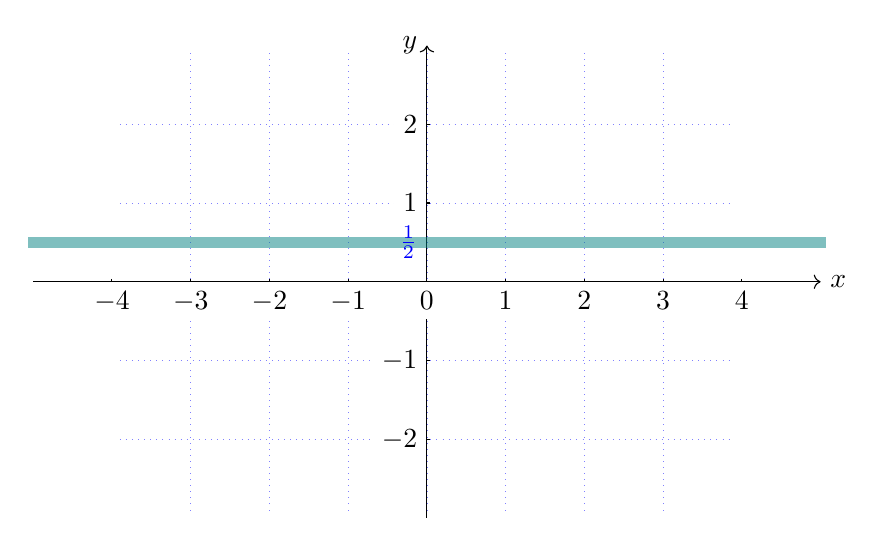
\begin{tikzpicture}

% Styles
\tikzstyle{axes}=[]
\tikzstyle help lines=[color=blue!50,very thin,dotted]


%%%%%%%%%%%%%%%%%%%%%%%%%%%%%%%%
%		GRID
%%%%%%%%%%%%%%%%%%%%%%%%%%%%%%%%

\draw[style=help lines,step=1cm] (-3.9,-2.9) grid (3.9,2.9);



%%%%%%%%%%%%%%%%%%%%%%%%%%%%%%%%
%		ASSENSTELSEL
%%%%%%%%%%%%%%%%%%%%%%%%%%%%%%%%

\draw[->] (-5,0) -- (5,0) node[right] {$x$};
\draw[->] (0,-3) -- (0,3) node[left]{$y$};

%\draw[fill,cyan](1,1)circle [radius=0.025];

%\draw[red,cap=rect, loosely dashed, ultra thick, domain=-2:2] plot (\x, {(\x*\x-1)+0.05}) node[above,yshift=-.7cm, right]{};

%%%%%%%%%%%%%%%%%%%%%%%%%%%%%%%%
%legende
%%%%%%%%%%%%%%%%%%%%%%%%%%%%%%%%
%\tkzDefPoint(0.5,3.5){A}
%\tkzDefPoint(1,3.5){B}
%\tkzLabelPoint[right,xshift=+0.1cm](B){${\color{cyan}f(x)=|x^2-1|}$}
%\tkzDrawSegment[cyan,ultra thick](A,B)

%\tkzDefPoint(0.5,3.2){C}
%\tkzDefPoint(1,3.2){D}
%\tkzLabelPoint[right,xshift=+0.1cm](D){${\color{red}e(x)=x^2-1}$}
%\tkzDrawSegment[red,cap=rect, loosely dashed, ultra thick](C,D)


%%%%%%%%%%%%%%%%%%%%%%%%%%%%%%%%
%getallen op de x-as en lijntjes
%%%%%%%%%%%%%%%%%%%%%%%%%%%%%%%%   
\foreach \x/\xtext in {-4,-3,-2,-1,0,1,2,3,4}
	\draw[xshift=\x cm] (0pt,1pt) -- (0pt,0pt) node[below,fill=white]
	{$\xtext$};,3
	
%getallen op de y-as en lijntjes  
%BEGIN LUS
\foreach \y/\ytext in {-2,-1,1,2}
	\draw[yshift=\y cm] (1pt,0pt) -- (0pt,0pt) node[left,fill=white]
	{$\ytext$}; %EINDE LUS



%%%%%%%%%%%%%%%%%%%%%%%%%%%%%%%%
%		GRAFIEKEN
%%%%%%%%%%%%%%%%%%%%%%%%%%%%%%%%
%\draw[cyan,cap=rect,thick, domain=-6:6] plot (\x, \x) node[above, right]{${\color{cyan}y=x}$};


\draw[teal,cap=rect,line width=4, opacity=.5, domain=-5:5] plot (\x, {
	0.5		% <- plaats het functievoorschrift hier
}) node[opacity=1,above]{};


 
%node[blue]{stijgen} 
%\draw[cyan,cap=rect,ultra thick, domain=2.25:6] plot (\x, {(\x-2)^(-1)}) node[above,yshift=+0.5cm,left]{$\color{cyan} y=\frac{1}{x-2}$};


%\draw[cyan,cap=rect,ultra thick, domain=-7:1.9] plot (\x, {exp{\x}}) node[above, right]{${\color{cyan}y=\exp{x}}$};

%%%%%%%%%%%%%%%%%%%%%%%%%%%%%%%%
%		MARKERINGEN
%%%%%%%%%%%%%%%%%%%%%%%%%%%%%%%%
%verticale lijn
%\draw[-o,line width=4,teal, cap=rect,opacity=0.3] (0,-4) -- (0,0.25) node[right] {};
%\draw[line width=4,teal, cap=rect,opacity=0.3] (0,0) -- (0,4.2) node[right] {bld $f$ = $\mathbb{R}_0$};
%horizontale lijn

% \draw[white,fill=blue,opacity=.5] (1,-2) circle [radius=.1]   node[blue, above,xshift=-1.1cm,opacity=1] {buigpunt in $(1,-2)$};


 


\draw[] (0,.5) node[blue,left] {$\frac{1}{2}$};
%\draw[] (1.5,-5) node[blue] {bol of convex};

\end{tikzpicture}
 
%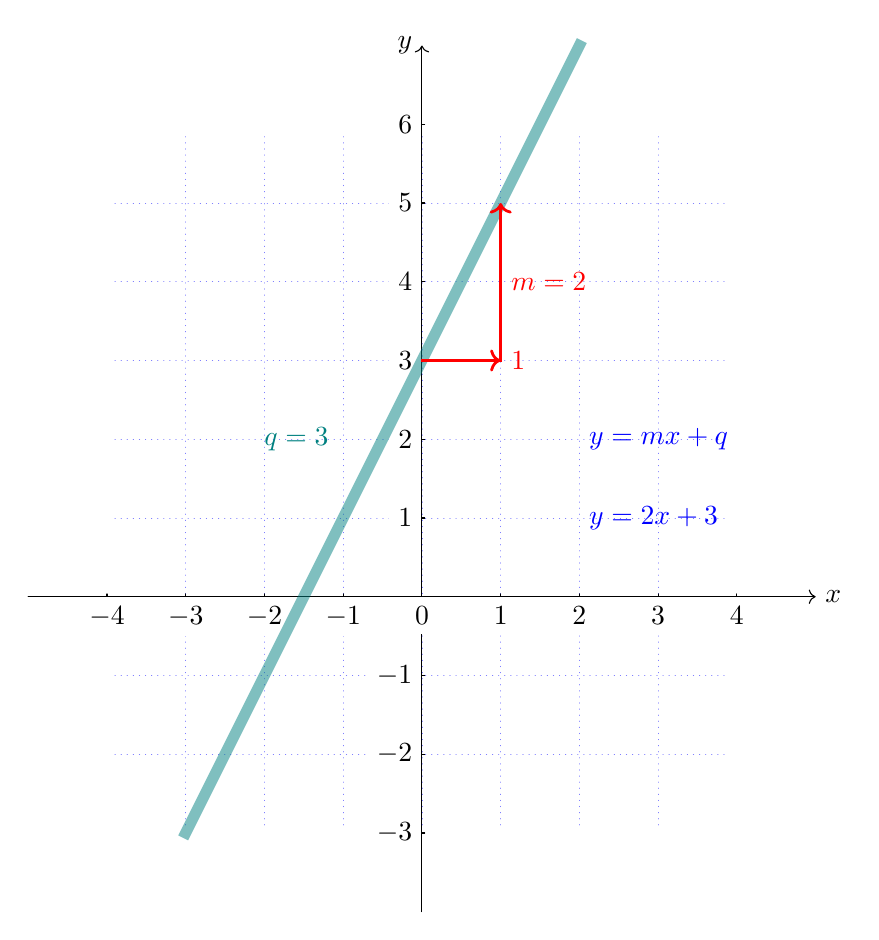
\begin{tikzpicture}[scale=1,cap=round]

% Styles
\tikzstyle{axes}=[]
\tikzstyle help lines=[color=blue!50,very thin,dotted]


%%%%%%%%%%%%%%%%%%%%%%%%%%%%%%%%
%		GRID
%%%%%%%%%%%%%%%%%%%%%%%%%%%%%%%%

\draw[style=help lines,step=1cm] (-3.9,-2.9) grid (3.9,5.9);



%%%%%%%%%%%%%%%%%%%%%%%%%%%%%%%%
%		ASSENSTELSEL
%%%%%%%%%%%%%%%%%%%%%%%%%%%%%%%%

\draw[->] (-5,0) -- (5,0) node[right] {$x$};
\draw[->] (0,-4) -- (0,7) node[left]{$y$};

%\draw[fill,cyan](1,1)circle [radius=0.025];

%\draw[red,cap=rect, loosely dashed, ultra thick, domain=-2:2] plot (\x, {(\x*\x-1)+0.05}) node[above,yshift=-.7cm, right]{};

%%%%%%%%%%%%%%%%%%%%%%%%%%%%%%%%
%legende
%%%%%%%%%%%%%%%%%%%%%%%%%%%%%%%%
%\tkzDefPoint(0.5,3.5){A}
%\tkzDefPoint(1,3.5){B}
%\tkzLabelPoint[right,xshift=+0.1cm](B){${\color{cyan}f(x)=|x^2-1|}$}
%\tkzDrawSegment[cyan,ultra thick](A,B)

%\tkzDefPoint(0.5,3.2){C}
%\tkzDefPoint(1,3.2){D}
%\tkzLabelPoint[right,xshift=+0.1cm](D){${\color{red}e(x)=x^2-1}$}
%\tkzDrawSegment[red,cap=rect, loosely dashed, ultra thick](C,D)


%%%%%%%%%%%%%%%%%%%%%%%%%%%%%%%%
%getallen op de x-as en lijntjes
%%%%%%%%%%%%%%%%%%%%%%%%%%%%%%%%   
\foreach \x/\xtext in {-4,-3,-2,-1,0,1,2,3,4}
	\draw[xshift=\x cm] (0pt,1pt) -- (0pt,0pt) node[below,fill=white]
	{$\xtext$};,3
	
%getallen op de y-as en lijntjes  
%BEGIN LUS
\foreach \y/\ytext in {-3,-2,-1,1,2,3,4,5,6}
	\draw[yshift=\y cm] (1pt,0pt) -- (0pt,0pt) node[left,fill=white]
	{$\ytext$}; %EINDE LUS



%%%%%%%%%%%%%%%%%%%%%%%%%%%%%%%%
%		GRAFIEKEN
%%%%%%%%%%%%%%%%%%%%%%%%%%%%%%%%
%\draw[cyan,cap=rect,thick, domain=-6:6] plot (\x, \x) node[above, right]{${\color{cyan}y=x}$};


\draw[teal,cap=rect,line width=4, opacity=.5, domain=-3:2] plot (\x, {
	2*\x + 3 		% <- plaats het functievoorschrift hier
}) node[opacity=1,left,pos=1,xshift=-1cm, yshift=+2cm]{$q=3$};
 
%node[blue]{stijgen} 
%\draw[cyan,cap=rect,ultra thick, domain=2.25:6] plot (\x, {(\x-2)^(-1)}) node[above,yshift=+0.5cm,left]{$\color{cyan} y=\frac{1}{x-2}$};


%\draw[cyan,cap=rect,ultra thick, domain=-7:1.9] plot (\x, {exp{\x}}) node[above, right]{${\color{cyan}y=\exp{x}}$};

%%%%%%%%%%%%%%%%%%%%%%%%%%%%%%%%
%		MARKERINGEN
%%%%%%%%%%%%%%%%%%%%%%%%%%%%%%%%
%verticale lijn
%\draw[-o,line width=4,teal, cap=rect,opacity=0.3] (0,-4) -- (0,0.25) node[right] {};
%\draw[line width=4,teal, cap=rect,opacity=0.3] (0,0) -- (0,4.2) node[right] {bld $f$ = $\mathbb{R}_0$};
%horizontale lijn

%horizontale lijn
\draw[->,line width=1,red, cap=rect,opacity=1] (0,3) -- (1,3) node[right] {$1$};
\draw[->,line width=1,red, cap=rect,opacity=1] (1,3) -- (1,5) node[right,pos=0.5] {$m=2$};



% \draw[white,fill=blue,opacity=.5] (1,-2) circle [radius=.1]   node[blue, above,xshift=-1.1cm,opacity=1] {buigpunt in $(1,-2)$};

\draw[] (2,2) node[blue,right] {$y=mx +q$};

\draw[] (2,1) node[blue,right] {$y=2x +3$};

\end{tikzpicture}
 
%
		\tikzsetfigurename{Fig_module_2_1_4_eerstegraadsfunctie_3}

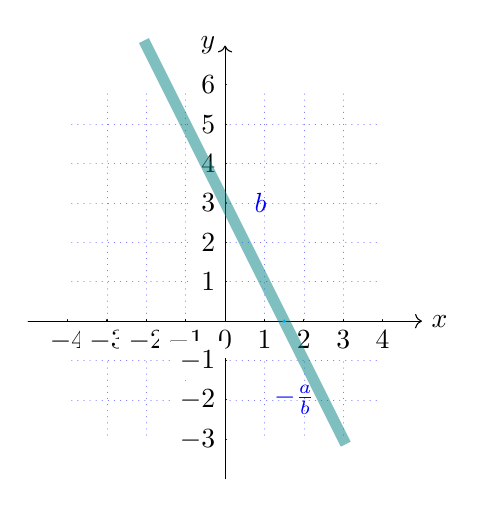
\begin{tikzpicture}[scale=.5,cap=round]

% Styles
\tikzstyle{axes}=[]
\tikzstyle help lines=[color=blue!50,very thin,dotted]


%%%%%%%%%%%%%%%%%%%%%%%%%%%%%%%%
%		GRID
%%%%%%%%%%%%%%%%%%%%%%%%%%%%%%%%

\draw[style=help lines,step=1cm] (-3.9,-2.9) grid (3.9,5.9);



%%%%%%%%%%%%%%%%%%%%%%%%%%%%%%%%
%		ASSENSTELSEL
%%%%%%%%%%%%%%%%%%%%%%%%%%%%%%%%

\draw[->] (-5,0) -- (5,0) node[right] {$x$};
\draw[->] (0,-4) -- (0,7) node[left]{$y$};

%\draw[fill,cyan](1,1)circle [radius=0.025];

%\draw[red,cap=rect, loosely dashed, ultra thick, domain=-2:2] plot (\x, {(\x*\x-1)+0.05}) node[above,yshift=-.7cm, right]{};

%%%%%%%%%%%%%%%%%%%%%%%%%%%%%%%%
%legende
%%%%%%%%%%%%%%%%%%%%%%%%%%%%%%%%
%\tkzDefPoint(0.5,3.5){A}
%\tkzDefPoint(1,3.5){B}
%\tkzLabelPoint[right,xshift=+0.1cm](B){${\color{cyan}f(x)=|x^2-1|}$}
%\tkzDrawSegment[cyan,ultra thick](A,B)

%\tkzDefPoint(0.5,3.2){C}
%\tkzDefPoint(1,3.2){D}
%\tkzLabelPoint[right,xshift=+0.1cm](D){${\color{red}e(x)=x^2-1}$}
%\tkzDrawSegment[red,cap=rect, loosely dashed, ultra thick](C,D)


%%%%%%%%%%%%%%%%%%%%%%%%%%%%%%%%
%getallen op de x-as en lijntjes
%%%%%%%%%%%%%%%%%%%%%%%%%%%%%%%%   
\foreach \x/\xtext in {-4,-3,-2,-1,0,1,2,3,4}
	\draw[xshift=\x cm] (0pt,1pt) -- (0pt,0pt) node[below,fill=white]
	{$\xtext$};,3
	
%getallen op de y-as en lijntjes  
%BEGIN LUS
\foreach \y/\ytext in {-3,-2,-1,1,2,3,4,5,6}
	\draw[yshift=\y cm] (1pt,0pt) -- (0pt,0pt) node[left,fill=white]
	{$\ytext$}; %EINDE LUS



%%%%%%%%%%%%%%%%%%%%%%%%%%%%%%%%
%		GRAFIEKEN
%%%%%%%%%%%%%%%%%%%%%%%%%%%%%%%%
%\draw[cyan,cap=rect,thick, domain=-6:6] plot (\x, \x) node[above, right]{${\color{cyan}y=x}$};


\draw[teal,cap=rect,line width=4, opacity=.5, domain=-2:3] plot (\x, {
	(-2)*\x + 3  		% <- plaats het functievoorschrift hier
}) node[opacity=1,left,pos=1,xshift=-1cm, yshift=+2cm]{};
 
%node[blue]{stijgen} 
%\draw[cyan,cap=rect,ultra thick, domain=2.25:6] plot (\x, {(\x-2)^(-1)}) node[above,yshift=+0.5cm,left]{$\color{cyan} y=\frac{1}{x-2}$};


%\draw[cyan,cap=rect,ultra thick, domain=-7:1.9] plot (\x, {exp{\x}}) node[above, right]{${\color{cyan}y=\exp{x}}$};

%%%%%%%%%%%%%%%%%%%%%%%%%%%%%%%%
%		MARKERINGEN
%%%%%%%%%%%%%%%%%%%%%%%%%%%%%%%%
%verticale lijn
%\draw[-o,line width=4,teal, cap=rect,opacity=0.3] (0,-4) -- (0,0.25) node[right] {};
%\draw[line width=4,teal, cap=rect,opacity=0.3] (0,0) -- (0,4.2) node[right] {bld $f$ = $\mathbb{R}_0$};
%horizontale lijn

%horizontale lijn
%\draw[->,line width=1,red, cap=rect,opacity=1] (0,3) -- (1,3) node[right] {$1$};
%\draw[->,line width=1,red, cap=rect,opacity=1] (1,3) -- (1,5) node[right,pos=0.5] {$m=2$};



% \draw[white,fill=blue,opacity=.5] (1,-2) circle [radius=.1]   node[blue, above,xshift=-1.1cm,opacity=1] {buigpunt in $(1,-2)$};

\draw[] (0.5,3) node[blue,right] {$b$};

\draw[fill,cyan](1.5,0)circle [radius=0.025];
\draw[] (1,-2) node[blue,right] {$-\frac{a}{b}$};

\end{tikzpicture}
 
%\tikzsetfigurename{Fig_module_2_1_4_rico_nul}

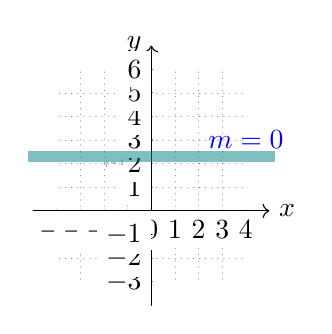
\begin{tikzpicture}[scale=0.3,cap=round]

% Styles
\tikzstyle{axes}=[]
\tikzstyle help lines=[color=blue!50,very thin,dotted]


%%%%%%%%%%%%%%%%%%%%%%%%%%%%%%%%
%		GRID
%%%%%%%%%%%%%%%%%%%%%%%%%%%%%%%%

\draw[style=help lines,step=1cm] (-3.9,-2.9) grid (3.9,5.9);



%%%%%%%%%%%%%%%%%%%%%%%%%%%%%%%%
%		ASSENSTELSEL
%%%%%%%%%%%%%%%%%%%%%%%%%%%%%%%%

\draw[->] (-5,0) -- (5,0) node[right] {$x$};
\draw[->] (0,-4) -- (0,7) node[left]{$y$};

%\draw[fill,cyan](1,1)circle [radius=0.025];

%\draw[red,cap=rect, loosely dashed, ultra thick, domain=-2:2] plot (\x, {(\x*\x-1)+0.05}) node[above,yshift=-.7cm, right]{};

%%%%%%%%%%%%%%%%%%%%%%%%%%%%%%%%
%legende
%%%%%%%%%%%%%%%%%%%%%%%%%%%%%%%%
%\tkzDefPoint(0.5,3.5){A}
%\tkzDefPoint(1,3.5){B}
%\tkzLabelPoint[right,xshift=+0.1cm](B){${\color{cyan}f(x)=|x^2-1|}$}
%\tkzDrawSegment[cyan,ultra thick](A,B)

%\tkzDefPoint(0.5,3.2){C}
%\tkzDefPoint(1,3.2){D}
%\tkzLabelPoint[right,xshift=+0.1cm](D){${\color{red}e(x)=x^2-1}$}
%\tkzDrawSegment[red,cap=rect, loosely dashed, ultra thick](C,D)


%%%%%%%%%%%%%%%%%%%%%%%%%%%%%%%%
%getallen op de x-as en lijntjes
%%%%%%%%%%%%%%%%%%%%%%%%%%%%%%%%   
\foreach \x/\xtext in {-4,-3,-2,-1,0,1,2,3,4}
	\draw[xshift=\x cm] (0pt,1pt) -- (0pt,0pt) node[below,fill=white]
	{$\xtext$};,3
	
%getallen op de y-as en lijntjes  
%BEGIN LUS
\foreach \y/\ytext in {-3,-2,-1,1,2,3,4,5,6}
	\draw[yshift=\y cm] (1pt,0pt) -- (0pt,0pt) node[left,fill=white]
	{$\ytext$}; %EINDE LUS



%%%%%%%%%%%%%%%%%%%%%%%%%%%%%%%%
%		GRAFIEKEN
%%%%%%%%%%%%%%%%%%%%%%%%%%%%%%%%
%\draw[cyan,cap=rect,thick, domain=-6:6] plot (\x, \x) node[above, right]{${\color{cyan}y=x}$};


\draw[teal,cap=rect,line width=4, opacity=.5, domain=-5:5] plot (\x, {
	2.3 		% <- plaats het functievoorschrift hier
}) node[opacity=1,left,pos=1,xshift=-1cm, yshift=+2cm]{$q=3$};
 
%node[blue]{stijgen} 
%\draw[cyan,cap=rect,ultra thick, domain=2.25:6] plot (\x, {(\x-2)^(-1)}) node[above,yshift=+0.5cm,left]{$\color{cyan} y=\frac{1}{x-2}$};


%\draw[cyan,cap=rect,ultra thick, domain=-7:1.9] plot (\x, {exp{\x}}) node[above, right]{${\color{cyan}y=\exp{x}}$};

%%%%%%%%%%%%%%%%%%%%%%%%%%%%%%%%
%		MARKERINGEN
%%%%%%%%%%%%%%%%%%%%%%%%%%%%%%%%
%verticale lijn
%\draw[-o,line width=4,teal, cap=rect,opacity=0.3] (0,-4) -- (0,0.25) node[right] {};
%\draw[line width=4,teal, cap=rect,opacity=0.3] (0,0) -- (0,4.2) node[right] {bld $f$ = $\mathbb{R}_0$};
%horizontale lijn

%horizontale lijn





% \draw[white,fill=blue,opacity=.5] (1,-2) circle [radius=.1]   node[blue, above,xshift=-1.1cm,opacity=1] {buigpunt in $(1,-2)$};

\draw[] (2,3) node[blue,right] {$m=0$};



\end{tikzpicture}
 
%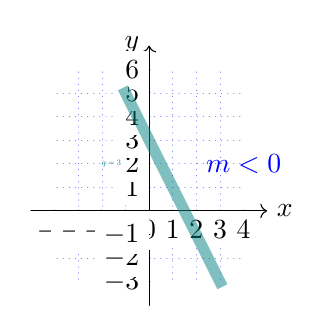
\begin{tikzpicture}[scale=0.3,cap=round]

% Styles
\tikzstyle{axes}=[]
\tikzstyle help lines=[color=blue!50,very thin,dotted]


%%%%%%%%%%%%%%%%%%%%%%%%%%%%%%%%
%		GRID
%%%%%%%%%%%%%%%%%%%%%%%%%%%%%%%%

\draw[style=help lines,step=1cm] (-3.9,-2.9) grid (3.9,5.9);



%%%%%%%%%%%%%%%%%%%%%%%%%%%%%%%%
%		ASSENSTELSEL
%%%%%%%%%%%%%%%%%%%%%%%%%%%%%%%%

\draw[->] (-5,0) -- (5,0) node[right] {$x$};
\draw[->] (0,-4) -- (0,7) node[left]{$y$};

%\draw[fill,cyan](1,1)circle [radius=0.025];

%\draw[red,cap=rect, loosely dashed, ultra thick, domain=-2:2] plot (\x, {(\x*\x-1)+0.05}) node[above,yshift=-.7cm, right]{};

%%%%%%%%%%%%%%%%%%%%%%%%%%%%%%%%
%legende
%%%%%%%%%%%%%%%%%%%%%%%%%%%%%%%%
%\tkzDefPoint(0.5,3.5){A}
%\tkzDefPoint(1,3.5){B}
%\tkzLabelPoint[right,xshift=+0.1cm](B){${\color{cyan}f(x)=|x^2-1|}$}
%\tkzDrawSegment[cyan,ultra thick](A,B)

%\tkzDefPoint(0.5,3.2){C}
%\tkzDefPoint(1,3.2){D}
%\tkzLabelPoint[right,xshift=+0.1cm](D){${\color{red}e(x)=x^2-1}$}
%\tkzDrawSegment[red,cap=rect, loosely dashed, ultra thick](C,D)


%%%%%%%%%%%%%%%%%%%%%%%%%%%%%%%%
%getallen op de x-as en lijntjes
%%%%%%%%%%%%%%%%%%%%%%%%%%%%%%%%   
\foreach \x/\xtext in {-4,-3,-2,-1,0,1,2,3,4}
	\draw[xshift=\x cm] (0pt,1pt) -- (0pt,0pt) node[below,fill=white]
	{$\xtext$};,3
	
%getallen op de y-as en lijntjes  
%BEGIN LUS
\foreach \y/\ytext in {-3,-2,-1,1,2,3,4,5,6}
	\draw[yshift=\y cm] (1pt,0pt) -- (0pt,0pt) node[left,fill=white]
	{$\ytext$}; %EINDE LUS



%%%%%%%%%%%%%%%%%%%%%%%%%%%%%%%%
%		GRAFIEKEN
%%%%%%%%%%%%%%%%%%%%%%%%%%%%%%%%
%\draw[cyan,cap=rect,thick, domain=-6:6] plot (\x, \x) node[above, right]{${\color{cyan}y=x}$};


\draw[teal,cap=rect,line width=4, opacity=.5, domain=-1:3] plot (\x, {
	(-2)*\x + 3  		% <- plaats het functievoorschrift hier
}) node[opacity=1,left,pos=1,xshift=-1cm, yshift=+2cm]{$q=3$};
 
%node[blue]{stijgen} 
%\draw[cyan,cap=rect,ultra thick, domain=2.25:6] plot (\x, {(\x-2)^(-1)}) node[above,yshift=+0.5cm,left]{$\color{cyan} y=\frac{1}{x-2}$};


%\draw[cyan,cap=rect,ultra thick, domain=-7:1.9] plot (\x, {exp{\x}}) node[above, right]{${\color{cyan}y=\exp{x}}$};

%%%%%%%%%%%%%%%%%%%%%%%%%%%%%%%%
%		MARKERINGEN
%%%%%%%%%%%%%%%%%%%%%%%%%%%%%%%%
%verticale lijn
%\draw[-o,line width=4,teal, cap=rect,opacity=0.3] (0,-4) -- (0,0.25) node[right] {};
%\draw[line width=4,teal, cap=rect,opacity=0.3] (0,0) -- (0,4.2) node[right] {bld $f$ = $\mathbb{R}_0$};
%horizontale lijn

%horizontale lijn




% \draw[white,fill=blue,opacity=.5] (1,-2) circle [radius=.1]   node[blue, above,xshift=-1.1cm,opacity=1] {buigpunt in $(1,-2)$};

\draw[] (2,2) node[blue,right] {$m<0$};



\end{tikzpicture}
 
%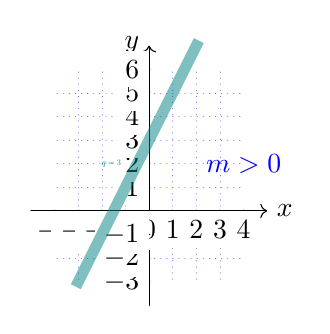
\begin{tikzpicture}[scale=0.3,cap=round]

% Styles
\tikzstyle{axes}=[]
\tikzstyle help lines=[color=blue!50,very thin,dotted]


%%%%%%%%%%%%%%%%%%%%%%%%%%%%%%%%
%		GRID
%%%%%%%%%%%%%%%%%%%%%%%%%%%%%%%%

\draw[style=help lines,step=1cm] (-3.9,-2.9) grid (3.9,5.9);



%%%%%%%%%%%%%%%%%%%%%%%%%%%%%%%%
%		ASSENSTELSEL
%%%%%%%%%%%%%%%%%%%%%%%%%%%%%%%%

\draw[->] (-5,0) -- (5,0) node[right] {$x$};
\draw[->] (0,-4) -- (0,7) node[left]{$y$};

%\draw[fill,cyan](1,1)circle [radius=0.025];

%\draw[red,cap=rect, loosely dashed, ultra thick, domain=-2:2] plot (\x, {(\x*\x-1)+0.05}) node[above,yshift=-.7cm, right]{};

%%%%%%%%%%%%%%%%%%%%%%%%%%%%%%%%
%legende
%%%%%%%%%%%%%%%%%%%%%%%%%%%%%%%%
%\tkzDefPoint(0.5,3.5){A}
%\tkzDefPoint(1,3.5){B}
%\tkzLabelPoint[right,xshift=+0.1cm](B){${\color{cyan}f(x)=|x^2-1|}$}
%\tkzDrawSegment[cyan,ultra thick](A,B)

%\tkzDefPoint(0.5,3.2){C}
%\tkzDefPoint(1,3.2){D}
%\tkzLabelPoint[right,xshift=+0.1cm](D){${\color{red}e(x)=x^2-1}$}
%\tkzDrawSegment[red,cap=rect, loosely dashed, ultra thick](C,D)


%%%%%%%%%%%%%%%%%%%%%%%%%%%%%%%%
%getallen op de x-as en lijntjes
%%%%%%%%%%%%%%%%%%%%%%%%%%%%%%%%   
\foreach \x/\xtext in {-4,-3,-2,-1,0,1,2,3,4}
	\draw[xshift=\x cm] (0pt,1pt) -- (0pt,0pt) node[below,fill=white]
	{$\xtext$};,3
	
%getallen op de y-as en lijntjes  
%BEGIN LUS
\foreach \y/\ytext in {-3,-2,-1,1,2,3,4,5,6}
	\draw[yshift=\y cm] (1pt,0pt) -- (0pt,0pt) node[left,fill=white]
	{$\ytext$}; %EINDE LUS



%%%%%%%%%%%%%%%%%%%%%%%%%%%%%%%%
%		GRAFIEKEN
%%%%%%%%%%%%%%%%%%%%%%%%%%%%%%%%
%\draw[cyan,cap=rect,thick, domain=-6:6] plot (\x, \x) node[above, right]{${\color{cyan}y=x}$};


\draw[teal,cap=rect,line width=4, opacity=.5, domain=-3:2] plot (\x, {
	2*\x + 3 		% <- plaats het functievoorschrift hier
}) node[opacity=1,left,pos=1,xshift=-1cm, yshift=+2cm]{$q=3$};
 
%node[blue]{stijgen} 
%\draw[cyan,cap=rect,ultra thick, domain=2.25:6] plot (\x, {(\x-2)^(-1)}) node[above,yshift=+0.5cm,left]{$\color{cyan} y=\frac{1}{x-2}$};


%\draw[cyan,cap=rect,ultra thick, domain=-7:1.9] plot (\x, {exp{\x}}) node[above, right]{${\color{cyan}y=\exp{x}}$};

%%%%%%%%%%%%%%%%%%%%%%%%%%%%%%%%
%		MARKERINGEN
%%%%%%%%%%%%%%%%%%%%%%%%%%%%%%%%
%verticale lijn
%\draw[-o,line width=4,teal, cap=rect,opacity=0.3] (0,-4) -- (0,0.25) node[right] {};
%\draw[line width=4,teal, cap=rect,opacity=0.3] (0,0) -- (0,4.2) node[right] {bld $f$ = $\mathbb{R}_0$};
%horizontale lijn

%horizontale lijn



% \draw[white,fill=blue,opacity=.5] (1,-2) circle [radius=.1]   node[blue, above,xshift=-1.1cm,opacity=1] {buigpunt in $(1,-2)$};

\draw[] (2,2) node[blue,right] {$ m > 0 $};



\end{tikzpicture}
 

%		\tikzsetfigurename{Fig_module_2_1_5_tweedegraadsfunctie_1}

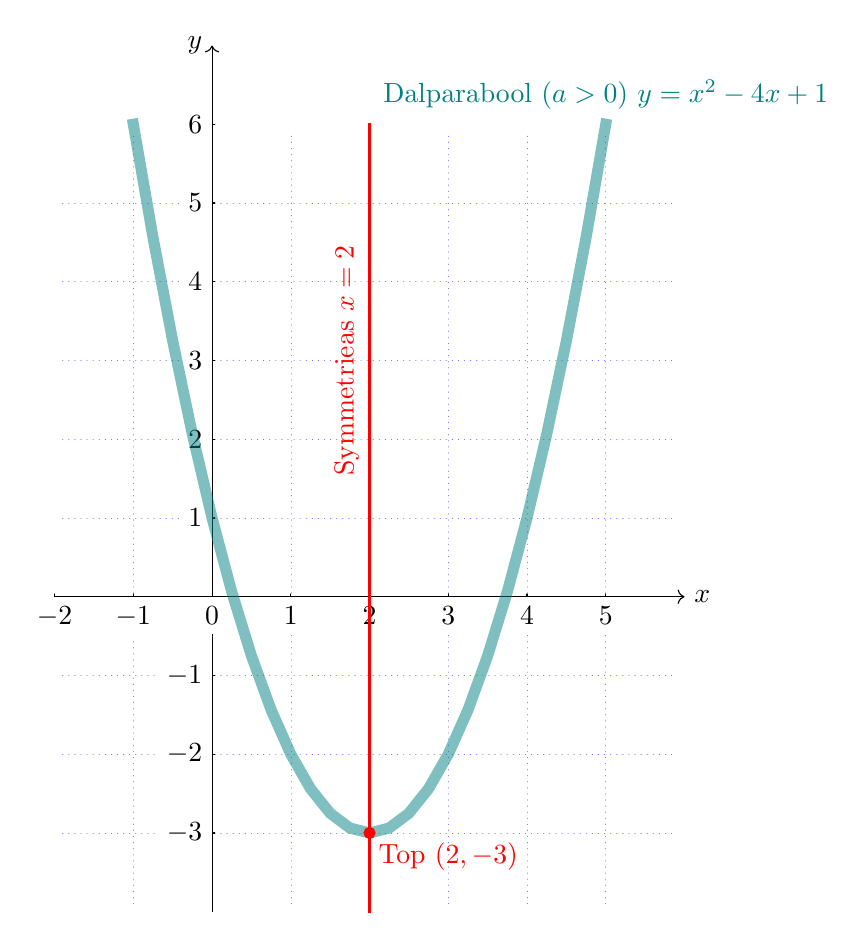
\begin{tikzpicture}[scale=1,cap=round]

% Styles
\tikzstyle{axes}=[]
\tikzstyle help lines=[color=blue!50,very thin,dotted]


%%%%%%%%%%%%%%%%%%%%%%%%%%%%%%%%
%		GRID
%%%%%%%%%%%%%%%%%%%%%%%%%%%%%%%%

\draw[style=help lines,step=1cm] (-1.9,-3.9) grid (5.9,5.9);



%%%%%%%%%%%%%%%%%%%%%%%%%%%%%%%%
%		ASSENSTELSEL
%%%%%%%%%%%%%%%%%%%%%%%%%%%%%%%%

\draw[->] (-2,0) -- (6,0) node[right] {$x$};
\draw[->] (0,-4) -- (0,7) node[left]{$y$};

%\draw[fill,cyan](1,1)circle [radius=0.025];

%\draw[red,cap=rect, loosely dashed, ultra thick, domain=-2:2] plot (\x, {(\x*\x-1)+0.05}) node[above,yshift=-.7cm, right]{};

%%%%%%%%%%%%%%%%%%%%%%%%%%%%%%%%
%legende
%%%%%%%%%%%%%%%%%%%%%%%%%%%%%%%%
%\tkzDefPoint(0.5,3.5){A}
%\tkzDefPoint(1,3.5){B}
%\tkzLabelPoint[right,xshift=+0.1cm](B){${\color{cyan}f(x)=|x^2-1|}$}
%\tkzDrawSegment[cyan,ultra thick](A,B)

%\tkzDefPoint(0.5,3.2){C}
%\tkzDefPoint(1,3.2){D}
%\tkzLabelPoint[right,xshift=+0.1cm](D){${\color{red}e(x)=x^2-1}$}
%\tkzDrawSegment[red,cap=rect, loosely dashed, ultra thick](C,D)


%%%%%%%%%%%%%%%%%%%%%%%%%%%%%%%%
%getallen op de x-as en lijntjes
%%%%%%%%%%%%%%%%%%%%%%%%%%%%%%%%   
\foreach \x/\xtext in {-2,-1,0,1,2,3,4,5}
	\draw[xshift=\x cm] (0pt,1pt) -- (0pt,0pt) node[below,fill=white]
	{$\xtext$};,3
	
%getallen op de y-as en lijntjes  
%BEGIN LUS
\foreach \y/\ytext in {-3,-2,-1,1,2,3,4,5,6}
	\draw[yshift=\y cm] (1pt,0pt) -- (0pt,0pt) node[left,fill=white]
	{$\ytext$}; %EINDE LUS



%%%%%%%%%%%%%%%%%%%%%%%%%%%%%%%%
%		GRAFIEKEN
%%%%%%%%%%%%%%%%%%%%%%%%%%%%%%%%
%\draw[cyan,cap=rect,thick, domain=-6:6] plot (\x, \x) node[above, right]{${\color{cyan}y=x}$};


\draw[teal,cap=rect,line width=4, opacity=.5, domain=-1:5] plot (\x, {
	pow(\x,2)-4*\x + 1  		% <- plaats het functievoorschrift hier
}) node[opacity=1,above]{Dalparabool ($a>0$) $y=x^2-4x+1$};
 
%node[blue]{stijgen} 
%\draw[cyan,cap=rect,ultra thick, domain=2.25:6] plot (\x, {(\x-2)^(-1)}) node[above,yshift=+0.5cm,left]{$\color{cyan} y=\frac{1}{x-2}$};


%\draw[cyan,cap=rect,ultra thick, domain=-7:1.9] plot (\x, {exp{\x}}) node[above, right]{${\color{cyan}y=\exp{x}}$};

%%%%%%%%%%%%%%%%%%%%%%%%%%%%%%%%
%		MARKERINGEN
%%%%%%%%%%%%%%%%%%%%%%%%%%%%%%%%
%verticale lijn
\draw[line width=1,red, cap=rect,opacity=1] (2,-4) -- (2,6) node[above,rotate=90,xshift=-3cm] {Symmetrieas $x=2$};
%\draw[line width=4,teal, cap=rect,opacity=0.3] (0,0) -- (0,4.2) node[right] {bld $f$ = $\mathbb{R}_0$};
%horizontale lijn

%horizontale lijn
%\draw[->,line width=1,red, cap=rect,opacity=1] (0,3) -- (1,3) node[right] {$1$};
%\draw[->,line width=1,red, cap=rect,opacity=1] (1,3) -- (1,5) node[right,pos=0.5] {$m=2$};



% \draw[white,fill=blue,opacity=.5] (1,-2) circle [radius=.1]   node[blue, above,xshift=-1.1cm,opacity=1] {buigpunt in $(1,-2)$};

%\draw[] (0.5,3) node[blue,right] {$b$};

\draw[fill,red](2,-3)circle [radius=0.07] node[red,below,xshift=+1cm] {Top $(2,-3)$};
%\draw[] (1,-2) node[blue,right] {$-\frac{a}{b}$};

\end{tikzpicture}
 


\begin{tabular}{|c|c|c|}
	\hline
	$D=b^2-4ac$&$a>0 $& $a<0$\\	
	&top onderaan&top bovenaan\\
	\hline
	$D>0$&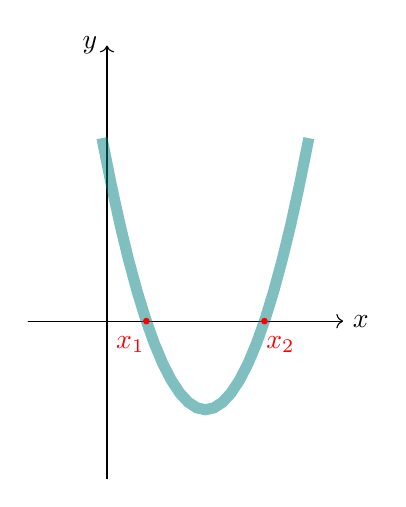
\begin{tikzpicture}[scale=0.5,cap=round]

% Styles
\tikzstyle{axes}=[]
\tikzstyle help lines=[color=blue!50,very thin,dotted]


%%%%%%%%%%%%%%%%%%%%%%%%%%%%%%%%
%		GRID
%%%%%%%%%%%%%%%%%%%%%%%%%%%%%%%%

%\draw[style=help lines,step=1cm] (-1.9,-3.9) grid (5.9,5.9);



%%%%%%%%%%%%%%%%%%%%%%%%%%%%%%%%
%		ASSENSTELSEL
%%%%%%%%%%%%%%%%%%%%%%%%%%%%%%%%

\draw[->] (-2,0) -- (6,0) node[right] {$x$};
\draw[->] (0,-4) -- (0,7) node[left]{$y$};

%\draw[fill,cyan](1,1)circle [radius=0.025];

%\draw[red,cap=rect, loosely dashed, ultra thick, domain=-2:2] plot (\x, {(\x*\x-1)+0.05}) node[above,yshift=-.7cm, right]{};

%%%%%%%%%%%%%%%%%%%%%%%%%%%%%%%%
%legende
%%%%%%%%%%%%%%%%%%%%%%%%%%%%%%%%
%\tkzDefPoint(0.5,3.5){A}
%\tkzDefPoint(1,3.5){B}
%\tkzLabelPoint[right,xshift=+0.1cm](B){${\color{cyan}f(x)=|x^2-1|}$}
%\tkzDrawSegment[cyan,ultra thick](A,B)

%\tkzDefPoint(0.5,3.2){C}
%\tkzDefPoint(1,3.2){D}
%\tkzLabelPoint[right,xshift=+0.1cm](D){${\color{red}e(x)=x^2-1}$}
%\tkzDrawSegment[red,cap=rect, loosely dashed, ultra thick](C,D)


%%%%%%%%%%%%%%%%%%%%%%%%%%%%%%%%
%getallen op de x-as en lijntjes
%%%%%%%%%%%%%%%%%%%%%%%%%%%%%%%%   

%\foreach \x/\xtext in {-2,-1,0,1,2,3,4,5}
%	\draw[xshift=\x cm] (0pt,1pt) -- (0pt,0pt) node[below,fill=white]{}; 
	
%getallen op de y-as en lijntjes  
%BEGIN LUS
%\foreach \y/\ytext in {-3,-2,-1,1,2,3,4,5,6}
%	\draw[yshift=\y cm] (1pt,0pt) -- (0pt,0pt) node[left,fill=white]{}; 



%%%%%%%%%%%%%%%%%%%%%%%%%%%%%%%%
%		GRAFIEKEN
%%%%%%%%%%%%%%%%%%%%%%%%%%%%%%%%
%\draw[cyan,cap=rect,thick, domain=-6:6] plot (\x, \x) node[above, right]{${\color{cyan}y=x}$};


\draw[teal,cap=rect,line width=4, opacity=.5, domain=-0.1:5.1] plot (\x, {
	1*pow(\x,2)-5*\x + 4  		% <- plaats het functievoorschrift hier
}) node[opacity=1,above]{};
 
%node[blue]{stijgen} 
%\draw[cyan,cap=rect,ultra thick, domain=2.25:6] plot (\x, {(\x-2)^(-1)}) node[above,yshift=+0.5cm,left]{$\color{cyan} y=\frac{1}{x-2}$};


%\draw[cyan,cap=rect,ultra thick, domain=-7:1.9] plot (\x, {exp{\x}}) node[above, right]{${\color{cyan}y=\exp{x}}$};

%%%%%%%%%%%%%%%%%%%%%%%%%%%%%%%%
%		MARKERINGEN
%%%%%%%%%%%%%%%%%%%%%%%%%%%%%%%%
%verticale lijn
\draw[fill,red] (1,0) circle [radius=0.07]  node[below,left,yshift=-.3cm,xshift=+0.1cm] {$x_1$};
\draw[fill,red] (4,0) circle [radius=0.07]  node[below,right,yshift=-.3cm,xshift=-0.1cm] {$x_2$};
%\draw[line width=4,teal, cap=rect,opacity=0.3] (0,0) -- (0,4.2) node[right] {bld $f$ = $\mathbb{R}_0$};
%horizontale lijn

%horizontale lijn
%\draw[->,line width=1,red, cap=rect,opacity=1] (0,3) -- (1,3) node[right] {$1$};
%\draw[->,line width=1,red, cap=rect,opacity=1] (1,3) -- (1,5) node[right,pos=0.5] {$m=2$};



% \draw[white,fill=blue,opacity=.5] (1,-2) circle [radius=.1]   node[blue, above,xshift=-1.1cm,opacity=1] {buigpunt in $(1,-2)$};

%\draw[] (0.5,3) node[blue,right] {$b$};

%\draw[fill,red](2,-3)circle [radius=0.07] node[red,below,xshift=+1cm] {Top $(2,-3)$};
%\draw[] (1,-2) node[blue,right] {$-\frac{a}{b}$};

\end{tikzpicture}
 &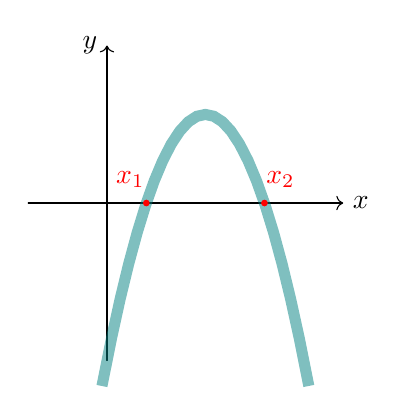
\begin{tikzpicture}[scale=0.5,cap=round]

% Styles
\tikzstyle{axes}=[]
\tikzstyle help lines=[color=blue!50,very thin,dotted]


%%%%%%%%%%%%%%%%%%%%%%%%%%%%%%%%
%		GRID
%%%%%%%%%%%%%%%%%%%%%%%%%%%%%%%%

%\draw[style=help lines,step=1cm] (-1.9,-3.9) grid (5.9,5.9);



%%%%%%%%%%%%%%%%%%%%%%%%%%%%%%%%
%		ASSENSTELSEL
%%%%%%%%%%%%%%%%%%%%%%%%%%%%%%%%

\draw[->] (-2,0) -- (6,0) node[right] {$x$};
\draw[->] (0,-4) -- (0,4) node[left]{$y$};

%\draw[fill,cyan](1,1)circle [radius=0.025];

%\draw[red,cap=rect, loosely dashed, ultra thick, domain=-2:2] plot (\x, {(\x*\x-1)+0.05}) node[above,yshift=-.7cm, right]{};

%%%%%%%%%%%%%%%%%%%%%%%%%%%%%%%%
%legende
%%%%%%%%%%%%%%%%%%%%%%%%%%%%%%%%
%\tkzDefPoint(0.5,3.5){A}
%\tkzDefPoint(1,3.5){B}
%\tkzLabelPoint[right,xshift=+0.1cm](B){${\color{cyan}f(x)=|x^2-1|}$}
%\tkzDrawSegment[cyan,ultra thick](A,B)

%\tkzDefPoint(0.5,3.2){C}
%\tkzDefPoint(1,3.2){D}
%\tkzLabelPoint[right,xshift=+0.1cm](D){${\color{red}e(x)=x^2-1}$}
%\tkzDrawSegment[red,cap=rect, loosely dashed, ultra thick](C,D)


%%%%%%%%%%%%%%%%%%%%%%%%%%%%%%%%
%getallen op de x-as en lijntjes
%%%%%%%%%%%%%%%%%%%%%%%%%%%%%%%%   

%\foreach \x/\xtext in {-2,-1,0,1,2,3,4,5}
	%\draw[xshift=\x cm] (0pt,1pt) -- (0pt,0pt) node[below,fill=white]{}; 
	
%getallen op de y-as en lijntjes  
%BEGIN LUS
%\foreach \y/\ytext in {-3,-2,-1,1,2,3,4,5,6}
%	\draw[yshift=\y cm] (1pt,0pt) -- (0pt,0pt) node[left,fill=white]{}; 



%%%%%%%%%%%%%%%%%%%%%%%%%%%%%%%%
%		GRAFIEKEN
%%%%%%%%%%%%%%%%%%%%%%%%%%%%%%%%
%\draw[cyan,cap=rect,thick, domain=-6:6] plot (\x, \x) node[above, right]{${\color{cyan}y=x}$};


\draw[teal,cap=rect,line width=4, opacity=.5, domain=-0.1:5.1] plot (\x, {
	(-1)*(pow(\x,2)-5*\x + 4)  		% <- plaats het functievoorschrift hier
}) node[opacity=1,above]{};
 
%node[blue]{stijgen} 
%\draw[cyan,cap=rect,ultra thick, domain=2.25:6] plot (\x, {(\x-2)^(-1)}) node[above,yshift=+0.5cm,left]{$\color{cyan} y=\frac{1}{x-2}$};


%\draw[cyan,cap=rect,ultra thick, domain=-7:1.9] plot (\x, {exp{\x}}) node[above, right]{${\color{cyan}y=\exp{x}}$};

%%%%%%%%%%%%%%%%%%%%%%%%%%%%%%%%
%		MARKERINGEN
%%%%%%%%%%%%%%%%%%%%%%%%%%%%%%%%
%verticale lijn
\draw[fill,red] (1,0) circle [radius=0.07]  node[below,left,yshift=+.3cm,xshift=0.1cm] {$x_1$};
\draw[fill,red] (4,0) circle [radius=0.07]  node[below,right,yshift=+.3cm,xshift=-0.1cm] {$x_2$};
%\draw[line width=4,teal, cap=rect,opacity=0.3] (0,0) -- (0,4.2) node[right] {bld $f$ = $\mathbb{R}_0$};
%horizontale lijn

%horizontale lijn
%\draw[->,line width=1,red, cap=rect,opacity=1] (0,3) -- (1,3) node[right] {$1$};
%\draw[->,line width=1,red, cap=rect,opacity=1] (1,3) -- (1,5) node[right,pos=0.5] {$m=2$};



% \draw[white,fill=blue,opacity=.5] (1,-2) circle [radius=.1]   node[blue, above,xshift=-1.1cm,opacity=1] {buigpunt in $(1,-2)$};

%\draw[] (0.5,3) node[blue,right] {$b$};

%\draw[fill,red](2,-3)circle [radius=0.07] node[red,below,xshift=+1cm] {Top $(2,-3)$};
%\draw[] (1,-2) node[blue,right] {$-\frac{a}{b}$};

\end{tikzpicture}
 \\
	\hline
	$D=0$&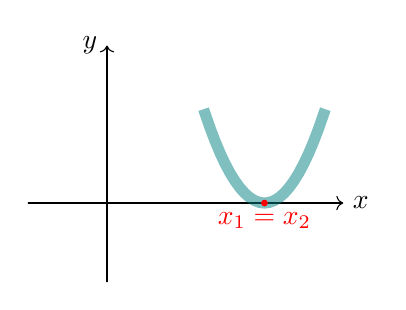
\begin{tikzpicture}[scale=0.5,cap=round]

% Styles
\tikzstyle{axes}=[]
\tikzstyle help lines=[color=blue!50,very thin,dotted]


%%%%%%%%%%%%%%%%%%%%%%%%%%%%%%%%
%		GRID
%%%%%%%%%%%%%%%%%%%%%%%%%%%%%%%%

%\draw[style=help lines,step=1cm] (-1.9,-3.9) grid (5.9,5.9);



%%%%%%%%%%%%%%%%%%%%%%%%%%%%%%%%
%		ASSENSTELSEL
%%%%%%%%%%%%%%%%%%%%%%%%%%%%%%%%

\draw[->] (-2,0) -- (6,0) node[right] {$x$};
\draw[->] (0,-2) -- (0,4) node[left]{$y$};

%\draw[fill,cyan](1,1)circle [radius=0.025];

%\draw[red,cap=rect, loosely dashed, ultra thick, domain=-2:2] plot (\x, {(\x*\x-1)+0.05}) node[above,yshift=-.7cm, right]{};

%%%%%%%%%%%%%%%%%%%%%%%%%%%%%%%%
%legende
%%%%%%%%%%%%%%%%%%%%%%%%%%%%%%%%
%\tkzDefPoint(0.5,3.5){A}
%\tkzDefPoint(1,3.5){B}
%\tkzLabelPoint[right,xshift=+0.1cm](B){${\color{cyan}f(x)=|x^2-1|}$}
%\tkzDrawSegment[cyan,ultra thick](A,B)

%\tkzDefPoint(0.5,3.2){C}
%\tkzDefPoint(1,3.2){D}
%\tkzLabelPoint[right,xshift=+0.1cm](D){${\color{red}e(x)=x^2-1}$}
%\tkzDrawSegment[red,cap=rect, loosely dashed, ultra thick](C,D)


%%%%%%%%%%%%%%%%%%%%%%%%%%%%%%%%
%getallen op de x-as en lijntjes
%%%%%%%%%%%%%%%%%%%%%%%%%%%%%%%%   

%\foreach \x/\xtext in {-2,-1,0,1,2,3,4,5}
%	\draw[xshift=\x cm] (0pt,1pt) -- (0pt,0pt) node[below,fill=white]{}; 
	
%getallen op de y-as en lijntjes  
%BEGIN LUS
%\foreach \y/\ytext in {-3,-2,-1,1,2,3,4,5,6}
%	\draw[yshift=\y cm] (1pt,0pt) -- (0pt,0pt) node[left,fill=white]{}; 



%%%%%%%%%%%%%%%%%%%%%%%%%%%%%%%%
%		GRAFIEKEN
%%%%%%%%%%%%%%%%%%%%%%%%%%%%%%%%
%\draw[cyan,cap=rect,thick, domain=-6:6] plot (\x, \x) node[above, right]{${\color{cyan}y=x}$};


\draw[teal,cap=rect,line width=4, opacity=.5, domain=2.5:5.5] plot (\x, {
	pow(\x-4,2)  		% <- plaats het functievoorschrift hier
}) node[opacity=1,above]{};
 
%node[blue]{stijgen} 
%\draw[cyan,cap=rect,ultra thick, domain=2.25:6] plot (\x, {(\x-2)^(-1)}) node[above,yshift=+0.5cm,left]{$\color{cyan} y=\frac{1}{x-2}$};


%\draw[cyan,cap=rect,ultra thick, domain=-7:1.9] plot (\x, {exp{\x}}) node[above, right]{${\color{cyan}y=\exp{x}}$};

%%%%%%%%%%%%%%%%%%%%%%%%%%%%%%%%
%		MARKERINGEN
%%%%%%%%%%%%%%%%%%%%%%%%%%%%%%%%
%verticale lijn
%draw[fill,red] (1,0) circle [radius=0.07]  node[below,left,yshift=-.3cm,xshift=+0.2cm] {$x_1$};
\draw[fill,red] (4,0) circle [radius=0.07]  node[below,yshift=0cm,xshift=0cm] {$x_1=x_2$};
%\draw[line width=4,teal, cap=rect,opacity=0.3] (0,0) -- (0,4.2) node[right] {bld $f$ = $\mathbb{R}_0$};
%horizontale lijn

%horizontale lijn
%\draw[->,line width=1,red, cap=rect,opacity=1] (0,3) -- (1,3) node[right] {$1$};
%\draw[->,line width=1,red, cap=rect,opacity=1] (1,3) -- (1,5) node[right,pos=0.5] {$m=2$};



% \draw[white,fill=blue,opacity=.5] (1,-2) circle [radius=.1]   node[blue, above,xshift=-1.1cm,opacity=1] {buigpunt in $(1,-2)$};

%\draw[] (0.5,3) node[blue,right] {$b$};

%\draw[fill,red](2,-3)circle [radius=0.07] node[red,below,xshift=+1cm] {Top $(2,-3)$};
%\draw[] (1,-2) node[blue,right] {$-\frac{a}{b}$};

\end{tikzpicture}
 &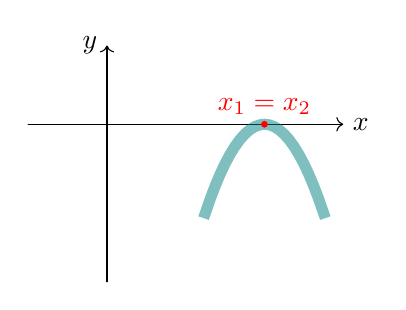
\begin{tikzpicture}[scale=0.5,cap=round]

% Styles
\tikzstyle{axes}=[]
\tikzstyle help lines=[color=blue!50,very thin,dotted]


%%%%%%%%%%%%%%%%%%%%%%%%%%%%%%%%
%		GRID
%%%%%%%%%%%%%%%%%%%%%%%%%%%%%%%%

%\draw[style=help lines,step=1cm] (-1.9,-3.9) grid (5.9,5.9);



%%%%%%%%%%%%%%%%%%%%%%%%%%%%%%%%
%		ASSENSTELSEL
%%%%%%%%%%%%%%%%%%%%%%%%%%%%%%%%

\draw[->] (-2,0) -- (6,0) node[right] {$x$};
\draw[->] (0,-4) -- (0,2) node[left]{$y$};

%\draw[fill,cyan](1,1)circle [radius=0.025];

%\draw[red,cap=rect, loosely dashed, ultra thick, domain=-2:2] plot (\x, {(\x*\x-1)+0.05}) node[above,yshift=-.7cm, right]{};

%%%%%%%%%%%%%%%%%%%%%%%%%%%%%%%%
%legende
%%%%%%%%%%%%%%%%%%%%%%%%%%%%%%%%
%\tkzDefPoint(0.5,3.5){A}
%\tkzDefPoint(1,3.5){B}
%\tkzLabelPoint[right,xshift=+0.1cm](B){${\color{cyan}f(x)=|x^2-1|}$}
%\tkzDrawSegment[cyan,ultra thick](A,B)

%\tkzDefPoint(0.5,3.2){C}
%\tkzDefPoint(1,3.2){D}
%\tkzLabelPoint[right,xshift=+0.1cm](D){${\color{red}e(x)=x^2-1}$}
%\tkzDrawSegment[red,cap=rect, loosely dashed, ultra thick](C,D)


%%%%%%%%%%%%%%%%%%%%%%%%%%%%%%%%
%getallen op de x-as en lijntjes
%%%%%%%%%%%%%%%%%%%%%%%%%%%%%%%%   

%\foreach \x/\xtext in {-2,-1,0,1,2,3,4,5}
%	\draw[xshift=\x cm] (0pt,1pt) -- (0pt,0pt) node[below,fill=white]{}; 
	
%getallen op de y-as en lijntjes  
%BEGIN LUS
%\foreach \y/\ytext in {-3,-2,-1,1,2,3,4,5,6}
%	\draw[yshift=\y cm] (1pt,0pt) -- (0pt,0pt) node[left,fill=white]{}; 



%%%%%%%%%%%%%%%%%%%%%%%%%%%%%%%%
%		GRAFIEKEN
%%%%%%%%%%%%%%%%%%%%%%%%%%%%%%%%
%\draw[cyan,cap=rect,thick, domain=-6:6] plot (\x, \x) node[above, right]{${\color{cyan}y=x}$};


\draw[teal,cap=rect,line width=4, opacity=.5, domain=2.5:5.5] plot (\x, {
	(-1)*pow(\x-4,2)  		% <- plaats het functievoorschrift hier
}) node[opacity=1,above]{};
 
%node[blue]{stijgen} 
%\draw[cyan,cap=rect,ultra thick, domain=2.25:6] plot (\x, {(\x-2)^(-1)}) node[above,yshift=+0.5cm,left]{$\color{cyan} y=\frac{1}{x-2}$};


%\draw[cyan,cap=rect,ultra thick, domain=-7:1.9] plot (\x, {exp{\x}}) node[above, right]{${\color{cyan}y=\exp{x}}$};

%%%%%%%%%%%%%%%%%%%%%%%%%%%%%%%%
%		MARKERINGEN
%%%%%%%%%%%%%%%%%%%%%%%%%%%%%%%%
%verticale lijn
%draw[fill,red] (1,0) circle [radius=0.07]  node[below,left,yshift=-.3cm,xshift=+0.2cm] {$x_1$};
\draw[fill,red] (4,0) circle [radius=0.07]  node[above,yshift=0cm,xshift=0cm] {$x_1=x_2$};
%\draw[line width=4,teal, cap=rect,opacity=0.3] (0,0) -- (0,4.2) node[right] {bld $f$ = $\mathbb{R}_0$};
%horizontale lijn

%horizontale lijn
%\draw[->,line width=1,red, cap=rect,opacity=1] (0,3) -- (1,3) node[right] {$1$};
%\draw[->,line width=1,red, cap=rect,opacity=1] (1,3) -- (1,5) node[right,pos=0.5] {$m=2$};



% \draw[white,fill=blue,opacity=.5] (1,-2) circle [radius=.1]   node[blue, above,xshift=-1.1cm,opacity=1] {buigpunt in $(1,-2)$};

%\draw[] (0.5,3) node[blue,right] {$b$};

%\draw[fill,red](2,-3)circle [radius=0.07] node[red,below,xshift=+1cm] {Top $(2,-3)$};
%\draw[] (1,-2) node[blue,right] {$-\frac{a}{b}$};

\end{tikzpicture}
 \\
	\hline
	$D<0$&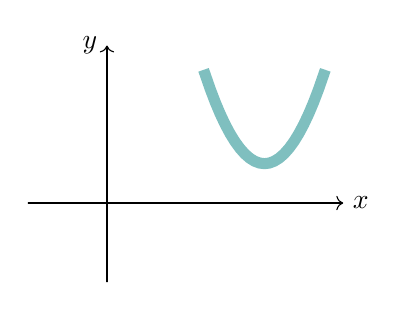
\begin{tikzpicture}[scale=0.5,cap=round]

% Styles
\tikzstyle{axes}=[]
\tikzstyle help lines=[color=blue!50,very thin,dotted]


%%%%%%%%%%%%%%%%%%%%%%%%%%%%%%%%
%		GRID
%%%%%%%%%%%%%%%%%%%%%%%%%%%%%%%%

%\draw[style=help lines,step=1cm] (-1.9,-3.9) grid (5.9,5.9);



%%%%%%%%%%%%%%%%%%%%%%%%%%%%%%%%
%		ASSENSTELSEL
%%%%%%%%%%%%%%%%%%%%%%%%%%%%%%%%

\draw[->] (-2,0) -- (6,0) node[right] {$x$};
\draw[->] (0,-2) -- (0,4) node[left]{$y$};

%\draw[fill,cyan](1,1)circle [radius=0.025];

%\draw[red,cap=rect, loosely dashed, ultra thick, domain=-2:2] plot (\x, {(\x*\x-1)+0.05}) node[above,yshift=-.7cm, right]{};

%%%%%%%%%%%%%%%%%%%%%%%%%%%%%%%%
%legende
%%%%%%%%%%%%%%%%%%%%%%%%%%%%%%%%
%\tkzDefPoint(0.5,3.5){A}
%\tkzDefPoint(1,3.5){B}
%\tkzLabelPoint[right,xshift=+0.1cm](B){${\color{cyan}f(x)=|x^2-1|}$}
%\tkzDrawSegment[cyan,ultra thick](A,B)

%\tkzDefPoint(0.5,3.2){C}
%\tkzDefPoint(1,3.2){D}
%\tkzLabelPoint[right,xshift=+0.1cm](D){${\color{red}e(x)=x^2-1}$}
%\tkzDrawSegment[red,cap=rect, loosely dashed, ultra thick](C,D)


%%%%%%%%%%%%%%%%%%%%%%%%%%%%%%%%
%getallen op de x-as en lijntjes
%%%%%%%%%%%%%%%%%%%%%%%%%%%%%%%%   

%\foreach \x/\xtext in {-2,-1,0,1,2,3,4,5}
%	\draw[xshift=\x cm] (0pt,1pt) -- (0pt,0pt) node[below,fill=white]{}; 
	
%getallen op de y-as en lijntjes  
%BEGIN LUS
%\foreach \y/\ytext in {-3,-2,-1,1,2,3,4,5,6}
%	\draw[yshift=\y cm] (1pt,0pt) -- (0pt,0pt) node[left,fill=white]{}; 



%%%%%%%%%%%%%%%%%%%%%%%%%%%%%%%%
%		GRAFIEKEN
%%%%%%%%%%%%%%%%%%%%%%%%%%%%%%%%
%\draw[cyan,cap=rect,thick, domain=-6:6] plot (\x, \x) node[above, right]{${\color{cyan}y=x}$};


\draw[teal,cap=rect,line width=4, opacity=.5, domain=2.5:5.5] plot (\x, {
	pow(\x-4,2)+1  		% <- plaats het functievoorschrift hier
}) node[opacity=1,above]{};
 
%node[blue]{stijgen} 
%\draw[cyan,cap=rect,ultra thick, domain=2.25:6] plot (\x, {(\x-2)^(-1)}) node[above,yshift=+0.5cm,left]{$\color{cyan} y=\frac{1}{x-2}$};


%\draw[cyan,cap=rect,ultra thick, domain=-7:1.9] plot (\x, {exp{\x}}) node[above, right]{${\color{cyan}y=\exp{x}}$};

%%%%%%%%%%%%%%%%%%%%%%%%%%%%%%%%
%		MARKERINGEN
%%%%%%%%%%%%%%%%%%%%%%%%%%%%%%%%
%verticale lijn
%draw[fill,red] (1,0) circle [radius=0.07]  node[below,left,yshift=-.3cm,xshift=+0.2cm] {$x_1$};
%\draw[fill,red] (4,0) circle [radius=0.07]  node[below,yshift=0cm,xshift=0cm] {$x_1=x_2$};
%\draw[line width=4,teal, cap=rect,opacity=0.3] (0,0) -- (0,4.2) node[right] {bld $f$ = $\mathbb{R}_0$};
%horizontale lijn

%horizontale lijn
%\draw[->,line width=1,red, cap=rect,opacity=1] (0,3) -- (1,3) node[right] {$1$};
%\draw[->,line width=1,red, cap=rect,opacity=1] (1,3) -- (1,5) node[right,pos=0.5] {$m=2$};



% \draw[white,fill=blue,opacity=.5] (1,-2) circle [radius=.1]   node[blue, above,xshift=-1.1cm,opacity=1] {buigpunt in $(1,-2)$};

%\draw[] (0.5,3) node[blue,right] {$b$};

%\draw[fill,red](2,-3)circle [radius=0.07] node[red,below,xshift=+1cm] {Top $(2,-3)$};
%\draw[] (1,-2) node[blue,right] {$-\frac{a}{b}$};

\end{tikzpicture}
 &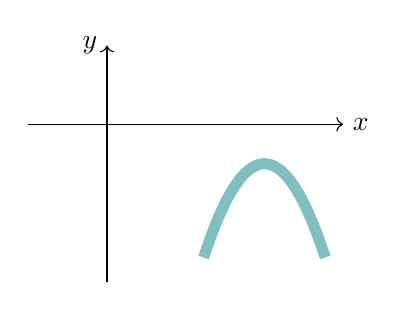
\begin{tikzpicture}[scale=0.5,cap=round]

% Styles
\tikzstyle{axes}=[]
\tikzstyle help lines=[color=blue!50,very thin,dotted]


%%%%%%%%%%%%%%%%%%%%%%%%%%%%%%%%
%		GRID
%%%%%%%%%%%%%%%%%%%%%%%%%%%%%%%%

%\draw[style=help lines,step=1cm] (-1.9,-3.9) grid (5.9,5.9);



%%%%%%%%%%%%%%%%%%%%%%%%%%%%%%%%
%		ASSENSTELSEL
%%%%%%%%%%%%%%%%%%%%%%%%%%%%%%%%

\draw[->] (-2,0) -- (6,0) node[right] {$x$};
\draw[->] (0,-4) -- (0,2) node[left]{$y$};

%\draw[fill,cyan](1,1)circle [radius=0.025];

%\draw[red,cap=rect, loosely dashed, ultra thick, domain=-2:2] plot (\x, {(\x*\x-1)+0.05}) node[above,yshift=-.7cm, right]{};

%%%%%%%%%%%%%%%%%%%%%%%%%%%%%%%%
%legende
%%%%%%%%%%%%%%%%%%%%%%%%%%%%%%%%
%\tkzDefPoint(0.5,3.5){A}
%\tkzDefPoint(1,3.5){B}
%\tkzLabelPoint[right,xshift=+0.1cm](B){${\color{cyan}f(x)=|x^2-1|}$}
%\tkzDrawSegment[cyan,ultra thick](A,B)

%\tkzDefPoint(0.5,3.2){C}
%\tkzDefPoint(1,3.2){D}
%\tkzLabelPoint[right,xshift=+0.1cm](D){${\color{red}e(x)=x^2-1}$}
%\tkzDrawSegment[red,cap=rect, loosely dashed, ultra thick](C,D)


%%%%%%%%%%%%%%%%%%%%%%%%%%%%%%%%
%getallen op de x-as en lijntjes
%%%%%%%%%%%%%%%%%%%%%%%%%%%%%%%%   

%\foreach \x/\xtext in {-2,-1,0,1,2,3,4,5}
%	\draw[xshift=\x cm] (0pt,1pt) -- (0pt,0pt) node[below,fill=white]{}; 
	
%getallen op de y-as en lijntjes  
%BEGIN LUS
%\foreach \y/\ytext in {-3,-2,-1,1,2,3,4,5,6}
%	\draw[yshift=\y cm] (1pt,0pt) -- (0pt,0pt) node[left,fill=white]{}; 



%%%%%%%%%%%%%%%%%%%%%%%%%%%%%%%%
%		GRAFIEKEN
%%%%%%%%%%%%%%%%%%%%%%%%%%%%%%%%
%\draw[cyan,cap=rect,thick, domain=-6:6] plot (\x, \x) node[above, right]{${\color{cyan}y=x}$};


\draw[teal,cap=rect,line width=4, opacity=.5, domain=2.5:5.5] plot (\x, {
	(-1)*pow(\x-4,2)-1  		% <- plaats het functievoorschrift hier
}) node[opacity=1,above]{};
 
%node[blue]{stijgen} 
%\draw[cyan,cap=rect,ultra thick, domain=2.25:6] plot (\x, {(\x-2)^(-1)}) node[above,yshift=+0.5cm,left]{$\color{cyan} y=\frac{1}{x-2}$};


%\draw[cyan,cap=rect,ultra thick, domain=-7:1.9] plot (\x, {exp{\x}}) node[above, right]{${\color{cyan}y=\exp{x}}$};

%%%%%%%%%%%%%%%%%%%%%%%%%%%%%%%%
%		MARKERINGEN
%%%%%%%%%%%%%%%%%%%%%%%%%%%%%%%%
%verticale lijn
%draw[fill,red] (1,0) circle [radius=0.07]  node[below,left,yshift=-.3cm,xshift=+0.2cm] {$x_1$};
%\draw[fill,red] (4,0) circle [radius=0.07]  node[below,yshift=0cm,xshift=0cm] {$x_1=x_2$};
%\draw[line width=4,teal, cap=rect,opacity=0.3] (0,0) -- (0,4.2) node[right] {bld $f$ = $\mathbb{R}_0$};
%horizontale lijn

%horizontale lijn
%\draw[->,line width=1,red, cap=rect,opacity=1] (0,3) -- (1,3) node[right] {$1$};
%\draw[->,line width=1,red, cap=rect,opacity=1] (1,3) -- (1,5) node[right,pos=0.5] {$m=2$};



% \draw[white,fill=blue,opacity=.5] (1,-2) circle [radius=.1]   node[blue, above,xshift=-1.1cm,opacity=1] {buigpunt in $(1,-2)$};

%\draw[] (0.5,3) node[blue,right] {$b$};

%\draw[fill,red](2,-3)circle [radius=0.07] node[red,below,xshift=+1cm] {Top $(2,-3)$};
%\draw[] (1,-2) node[blue,right] {$-\frac{a}{b}$};

\end{tikzpicture}
 \\
	\hline
\end{tabular}
%\tikzsetfigurename{Fig_module_2_1_5_tweedegraadsfunctie_3}

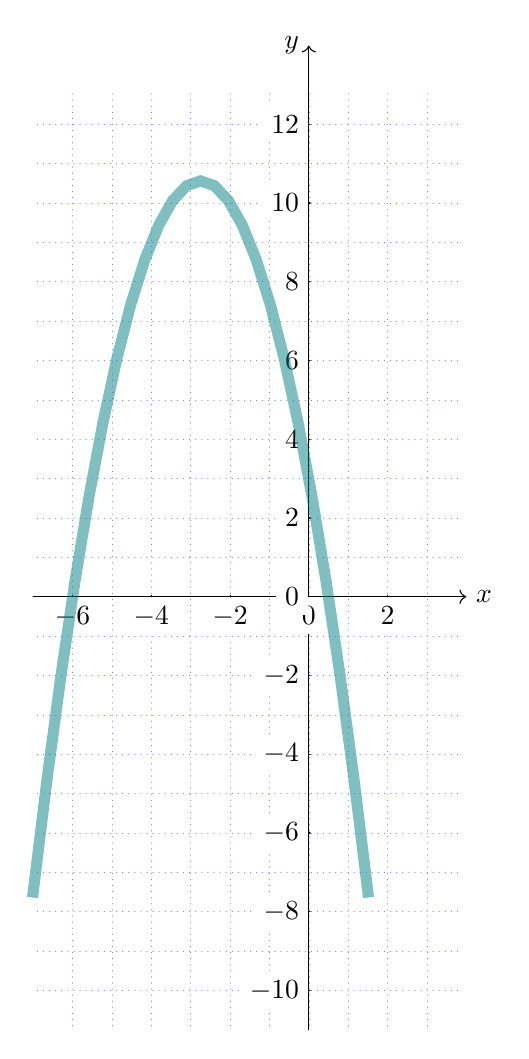
\begin{tikzpicture}[scale=0.5,cap=round]

% Styles
\tikzstyle{axes}=[]
\tikzstyle help lines=[color=blue!50,very thin,dotted]


%%%%%%%%%%%%%%%%%%%%%%%%%%%%%%%%
%		GRID
%%%%%%%%%%%%%%%%%%%%%%%%%%%%%%%%

\draw[style=help lines,step=1cm] (-6.9,-10.9) grid (3.9,12.9);



%%%%%%%%%%%%%%%%%%%%%%%%%%%%%%%%
%		ASSENSTELSEL
%%%%%%%%%%%%%%%%%%%%%%%%%%%%%%%%

\draw[->] (-7,0) -- (4,0) node[right] {$x$};
\draw[->] (0,-11) -- (0,14) node[left]{$y$};

%\draw[fill,cyan](1,1)circle [radius=0.025];

%\draw[red,cap=rect, loosely dashed, ultra thick, domain=-2:2] plot (\x, {(\x*\x-1)+0.05}) node[above,yshift=-.7cm, right]{};

%%%%%%%%%%%%%%%%%%%%%%%%%%%%%%%%
%legende
%%%%%%%%%%%%%%%%%%%%%%%%%%%%%%%%
%\tkzDefPoint(0.5,3.5){A}
%\tkzDefPoint(1,3.5){B}
%\tkzLabelPoint[right,xshift=+0.1cm](B){${\color{cyan}f(x)=|x^2-1|}$}
%\tkzDrawSegment[cyan,ultra thick](A,B)

%\tkzDefPoint(0.5,3.2){C}
%\tkzDefPoint(1,3.2){D}
%\tkzLabelPoint[right,xshift=+0.1cm](D){${\color{red}e(x)=x^2-1}$}
%\tkzDrawSegment[red,cap=rect, loosely dashed, ultra thick](C,D)


%%%%%%%%%%%%%%%%%%%%%%%%%%%%%%%%
%getallen op de x-as en lijntjes
%%%%%%%%%%%%%%%%%%%%%%%%%%%%%%%%   
\foreach \x/\xtext in {-6,-4,-2,0,2}
	\draw[xshift=\x cm] (0pt,1pt) -- (0pt,0pt) node[below,fill=white]
	{$\xtext$};,3
	
%getallen op de y-as en lijntjes  
%BEGIN LUS
\foreach \y/\ytext in {-10,-8,-6,-4,-2,0,2,4,6,8,10,12}
	\draw[yshift=\y cm] (1pt,0pt) -- (0pt,0pt) node[left,fill=white]
	{$\ytext$}; %EINDE LUS



%%%%%%%%%%%%%%%%%%%%%%%%%%%%%%%%
%		GRAFIEKEN
%%%%%%%%%%%%%%%%%%%%%%%%%%%%%%%%
%\draw[cyan,cap=rect,thick, domain=-6:6] plot (\x, \x) node[above, right]{${\color{cyan}y=x}$};


\draw[teal,cap=rect,line width=4, opacity=.5, domain=-7:1.5] plot (\x, {
	(-1)*(\x+6)*(\x-1/2)	% <- plaats het functievoorschrift hier
}) node[opacity=1,above]{};
 
%node[blue]{stijgen} 
%\draw[cyan,cap=rect,ultra thick, domain=2.25:6] plot (\x, {(\x-2)^(-1)}) node[above,yshift=+0.5cm,left]{$\color{cyan} y=\frac{1}{x-2}$};


%\draw[cyan,cap=rect,ultra thick, domain=-7:1.9] plot (\x, {exp{\x}}) node[above, right]{${\color{cyan}y=\exp{x}}$};

%%%%%%%%%%%%%%%%%%%%%%%%%%%%%%%%
%		MARKERINGEN
%%%%%%%%%%%%%%%%%%%%%%%%%%%%%%%%
%verticale lijn
%\draw[line width=1,red, cap=rect,opacity=1] (2,-4) -- (2,6) node[above,rotate=90,xshift=-3cm] {Symmetrieas $x=2$};
%\draw[line width=4,teal, cap=rect,opacity=0.3] (0,0) -- (0,4.2) node[right] {bld $f$ = $\mathbb{R}_0$};
%horizontale lijn

%horizontale lijn
%\draw[->,line width=1,red, cap=rect,opacity=1] (0,3) -- (1,3) node[right] {$1$};
%\draw[->,line width=1,red, cap=rect,opacity=1] (1,3) -- (1,5) node[right,pos=0.5] {$m=2$};



% \draw[white,fill=blue,opacity=.5] (1,-2) circle [radius=.1]   node[blue, above,xshift=-1.1cm,opacity=1] {buigpunt in $(1,-2)$};

%\draw[] (0.5,3) node[blue,right] {$b$};

%\draw[fill,red](2,-3)circle [radius=0.07] node[red,below,xshift=+1cm] {Top $(2,-3)$};
%\draw[] (1,-2) node[blue,right] {$-\frac{a}{b}$};

\end{tikzpicture}
 

%\tikzsetfigurename{Fig_module_2_1_7_veeltermfuncties_1}

\begin{center}
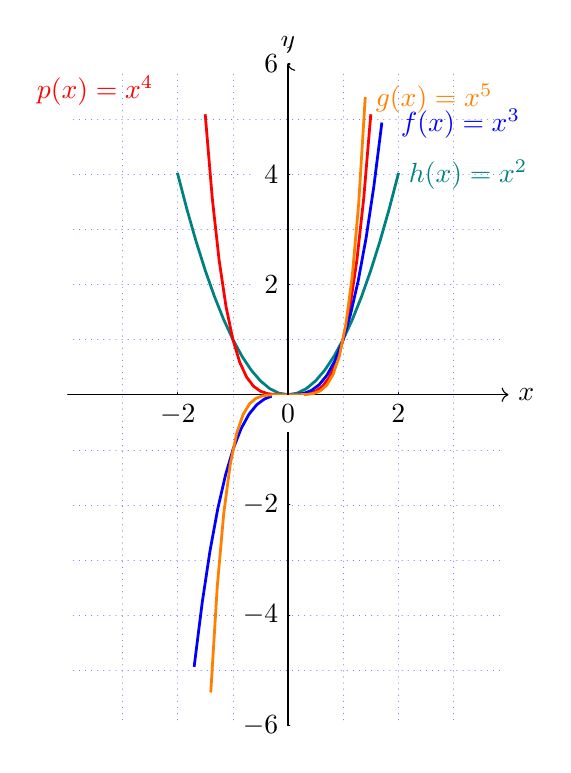
\begin{tikzpicture}[scale=0.7,cap=round]

% Styles
\tikzstyle{axes}=[]
\tikzstyle help lines=[color=blue!50,very thin,dotted]

% grid
\draw[style=help lines,step=1cm] (-3.9,-5.9) grid (3.9,5.9);

\draw[->] (-4,0) -- (4,0) node[right] {$x$};
\draw[->] (0,-6) -- (0,6) node[above] {$y$};

%\draw[fill,cyan](1,1)circle [radius=0.025];
%FUNCTIEVOORSCHRIFTEN



\draw[teal,cap=rect,line width=1, opacity=1, domain=-2:2] plot (\x, {
	pow(\x,2)  		% <- plaats het functievoorschrift hier
}) node[right,opacity=1]{$h(x)=x^2$};

\draw[red,cap=rect,line width=1, opacity=1, domain=-1.5:1.5] plot (\x, {
	pow(\x,4)  		% <- plaats het functievoorschrift hier
}) node[opacity=1,above,xshift=-3.5cm]{$p(x)=x^4$};

\draw[blue,cap=rect,line width=1, opacity=1, domain=-1.7:1.7] plot (\x, {
	pow(\x,3)  		% <- plaats het functievoorschrift hier
}) node[opacity=1,xshift=+1cm]{$f(x)=x^3$};

\draw[orange,cap=rect,line width=1, opacity=1, domain=-1.4:1.4] plot (\x, {
	pow(\x,5)  		% <- plaats het functievoorschrift hier
}) node[right,opacity=1]{$g(x)=x^5$};



%\draw[cyan,cap=rect,ultra thick, domain=1:2] plot (\x, {\x*\x-1}) node[above, right]{};
%\draw[red,cap=rect, loosely dashed, ultra thick, domain=-2:2] plot (\x, {(\x*\x-1)+0.05}) node[above,yshift=-.7cm, right]{};

%legende



%getallen op de x-as en lijntjes   
\foreach \x/\xtext in {-2,0,2}
	\draw[xshift=\x cm] (0pt,1pt) -- (0pt,0pt) node[below,fill=white]
	{$\xtext$};,3
	
%getallen op de y-as en lijntjes  
%BEGIN LUS
\foreach \y/\ytext in {-6,-4,-2,2,4,6}
	\draw[yshift=\y cm] (1pt,0pt) -- (0pt,0pt) node[left,fill=white]
	{$\ytext$}; %EINDE LUS



\end{tikzpicture}
\end{center}


%\tikzsetfigurename{Fig_module_2_1_7_veeltermfuncties_2}

\begin{center}
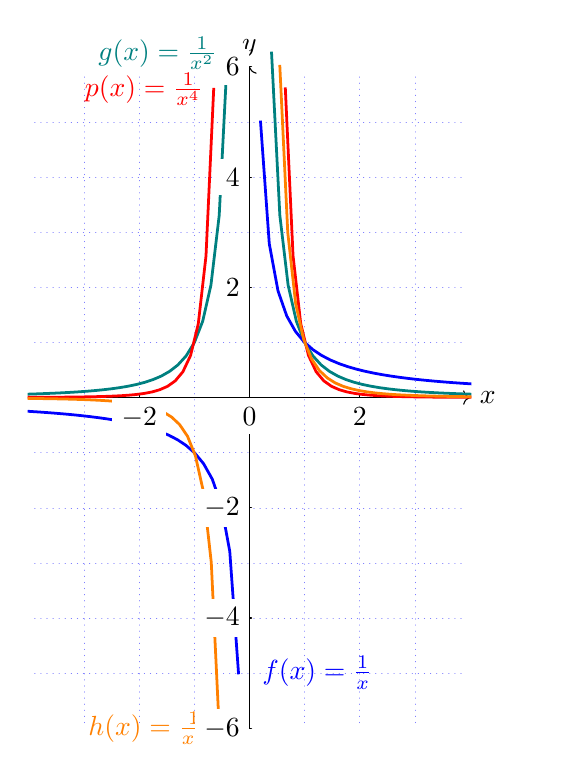
\begin{tikzpicture}[scale=0.7,cap=round]

% Styles
\tikzstyle{axes}=[]
\tikzstyle help lines=[color=blue!50,very thin,dotted]

% grid
\draw[style=help lines,step=1cm] (-3.9,-5.9) grid (3.9,5.9);

\draw[->] (-4,0) -- (4,0) node[right] {$x$};
\draw[->] (0,-6) -- (0,6) node[above] {$y$};

%\draw[fill,cyan](1,1)circle [radius=0.025];
%FUNCTIEVOORSCHRIFTEN


%------------------
\draw[teal,cap=rect,line width=1, opacity=1, domain=-4:-0.4] plot (\x, {
	pow(\x,-2)  		% <- plaats het functievoorschrift hier
}) node[left,opacity=1]{$g(x)=\frac{1}{x^2}$};
\draw[teal,cap=rect,line width=1, opacity=1, domain=0.4:4] plot (\x, {
	pow(\x,-2)  		% <- plaats het functievoorschrift hier
}) node[left,opacity=1]{};
%------------------

\draw[red,cap=rect,line width=1, opacity=1, domain=-4:-0.65] plot (\x, {
	pow(\x,-4)  		% <- plaats het functievoorschrift hier
}) node[opacity=1,left]{$p(x)=\frac{1}{x^4}$};
\draw[red,cap=rect,line width=1, opacity=1, domain=0.65:4] plot (\x, {
	pow(\x,-4)  		% <- plaats het functievoorschrift hier
}) node[opacity=1,left]{};
%------------------
\draw[blue,cap=rect,line width=1, opacity=1, domain=-4:-0.2] plot (\x, {
	pow(\x,-1)  		% <- plaats het functievoorschrift hier
}) node[opacity=1,xshift=+1cm]{$f(x)=\frac{1}{x}$};

\draw[blue,cap=rect,line width=1, opacity=1, domain=0.2:4] plot (\x, {
	pow(\x,-1)  		% <- plaats het functievoorschrift hier
}) node[opacity=1,xshift=+1cm]{};
%------------------
\draw[orange,cap=rect,line width=1, opacity=1, domain=-4:-0.55] plot (\x, {
	pow(\x,-3)  		% <- plaats het functievoorschrift hier
}) node[left,opacity=1]{$h(x)=\frac{1}{x^3}$};

\draw[orange,cap=rect,line width=1, opacity=1, domain=0.55:4] plot (\x, {
	pow(\x,-3)  		% <- plaats het functievoorschrift hier
}) node[left,opacity=1]{};

%------------------

%\draw[cyan,cap=rect,ultra thick, domain=1:2] plot (\x, {\x*\x-1}) node[above, right]{};
%\draw[red,cap=rect, loosely dashed, ultra thick, domain=-2:2] plot (\x, {(\x*\x-1)+0.05}) node[above,yshift=-.7cm, right]{};

%legende



%getallen op de x-as en lijntjes   
\foreach \x/\xtext in {-2,0,2}
	\draw[xshift=\x cm] (0pt,1pt) -- (0pt,0pt) node[below,fill=white]
	{$\xtext$};,3
	
%getallen op de y-as en lijntjes  
%BEGIN LUS
\foreach \y/\ytext in {-6,-4,-2,2,4,6}
	\draw[yshift=\y cm] (1pt,0pt) -- (0pt,0pt) node[left,fill=white]
	{$\ytext$}; %EINDE LUS



\end{tikzpicture}
\end{center}


%\tikzsetfigurename{Fig_module_2_1_7_veeltermfuncties_3}

\begin{center}
\begin{tikzpicture}[yscale=2,xscale=1]

% Styles
\tikzstyle{axes}=[]
\tikzstyle help lines=[color=blue!50,very thin,dotted]

% grid
\draw[style=help lines,step=1cm] (-.9,-2.4) grid (1.9,0.4);

\draw[->] (-1,0) -- (2,0) node[right] {$x$};
\draw[->] (0,-2.5) -- (0,0.5) node[above] {$y$};

%\draw[fill,cyan](1,1)circle [radius=0.025];
%FUNCTIEVOORSCHRIFTEN



\draw[teal,cap=rect,line width=1, opacity=1, domain=-0.5:1.8] plot (\x, {
	2*pow(\x,4)-3*pow(\x,3)-pow(\x,2)  		% <- plaats het functievoorschrift hier
}) node[left,opacity=1]{$f(x)=2x^4-3x^3-x^2$};



%\draw[cyan,cap=rect,ultra thick, domain=1:2] plot (\x, {\x*\x-1}) node[above, right]{};
%\draw[red,cap=rect, loosely dashed, ultra thick, domain=-2:2] plot (\x, {(\x*\x-1)+0.05}) node[above,yshift=-.7cm, right]{};

%legende



%getallen op de x-as en lijntjes   
\foreach \x/\xtext in {-1,1}
	\draw[xshift=\x cm] (0pt,1pt) -- (0pt,0pt) node[below,fill=white]
	{$\xtext$};,3
	
%getallen op de y-as en lijntjes  
%BEGIN LUS
\foreach \y/\ytext in {-4,-2,2}
	\draw[yshift=\y cm] (1pt,0pt) -- (0pt,0pt) node[left,fill=white]
	{$\ytext$}; %EINDE LUS



\end{tikzpicture}
\end{center}


\begin{center}
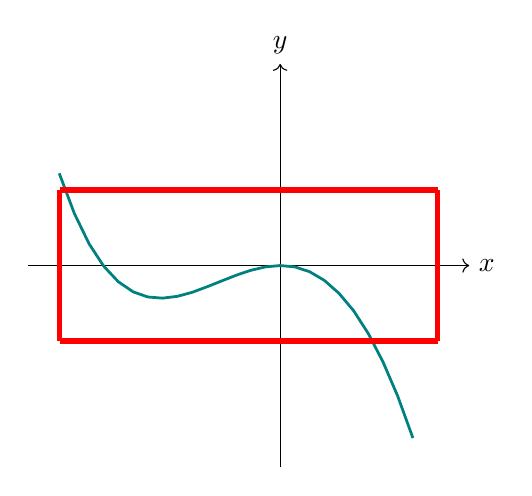
\begin{tikzpicture}[yscale=32,xscale=8]

% Styles
\tikzstyle{axes}=[]
\tikzstyle help lines=[color=blue!50,very thin,dotted]

% grid
%\draw[style=help lines,step=0.1cm] (-.9,-0.4) grid (0.9,0.4);

\draw[->] (-0.4,0) -- (0.3,0) node[right] {$x$};
\draw[->] (0,-0.08) -- (0,0.08) node[above] {$y$};

%\draw[fill,cyan](1,1)circle [radius=0.025];
%FUNCTIEVOORSCHRIFTEN



\draw[teal,cap=rect,line width=1, opacity=1, domain=-0.35:0.21] plot (\x, {
	2*pow(\x,4)-3*pow(\x,3)-pow(\x,2)  		% <- plaats het functievoorschrift hier
}) node[left,opacity=1]{};



%\draw[cyan,cap=rect,ultra thick, domain=1:2] plot (\x, {\x*\x-1}) node[above, right]{};
%\draw[red,cap=rect, loosely dashed, ultra thick, domain=-2:2] plot (\x, {(\x*\x-1)+0.05}) node[above,yshift=-.7cm, right]{};

%legende



%getallen op de x-as en lijntjes   
%\foreach \x/\xtext in {-.1,.1}
%	\draw[xshift=\x cm] (0pt,1pt) -- (0pt,0pt) node[below,fill=white]
%	{$$}; 
	
%getallen op de y-as en lijntjes  
%BEGIN LUS
%\foreach \y/\ytext in {-4,-2,2}
%	\draw[yshift=\y cm] (1pt,0pt) -- (0pt,0pt) node[left,fill=white]
%	{$$}; %EINDE LUS
\draw[color=red,line width=2] (-0.35,-0.03) -- (-0.35,0.03);
\draw[color=red,line width=2] (0.25,-0.03) -- (0.25,0.03);
\draw[color=red,line width=2] (-0.35,-0.03) -- (0.25,-0.03);
\draw[color=red,line width=2] (-0.35,0.03) -- (0.25,0.03);



\end{tikzpicture}
\end{center}


%\tikzsetfigurename{Fig_module_2_1_7_veeltermfuncties_4}

\begin{center}
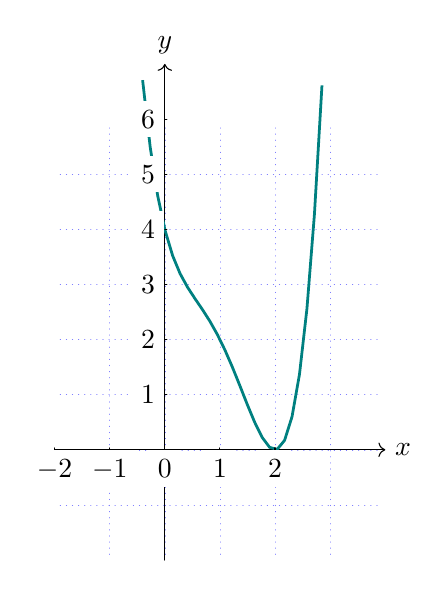
\begin{tikzpicture}[scale=0.7,cap=round]

% Styles
\tikzstyle{axes}=[]
\tikzstyle help lines=[color=blue!50,very thin,dotted]

% grid
\draw[style=help lines,step=1cm] (-1.9,-1.9) grid (3.9,5.9);

\draw[->] (-2,0) -- (4,0) node[right] {$x$};
\draw[->] (0,-2) -- (0,7) node[above] {$y$};

%\draw[fill,cyan](1,1)circle [radius=0.025];
%FUNCTIEVOORSCHRIFTEN


%------------------
\draw[teal,cap=rect,line width=1, opacity=1, domain=-0.4:2.85] plot (\x, {
	pow(\x,4)-4*pow(\x,3)+5*pow(\x,2)-4*\x+4   		% <- plaats het functievoorschrift hier
}) node[left,opacity=1]{};



%\draw[cyan,cap=rect,ultra thick, domain=1:2] plot (\x, {\x*\x-1}) node[above, right]{};
%\draw[red,cap=rect, loosely dashed, ultra thick, domain=-2:2] plot (\x, {(\x*\x-1)+0.05}) node[above,yshift=-.7cm, right]{};

%legende



%getallen op de x-as en lijntjes   
\foreach \x/\xtext in {-2,-1,0,1,2}
	\draw[xshift=\x cm] (0pt,1pt) -- (0pt,0pt) node[below,fill=white]
	{$\xtext$};,3
	
%getallen op de y-as en lijntjes  
%BEGIN LUS
\foreach \y/\ytext in {1,2,3,4,5,6}
	\draw[yshift=\y cm] (1pt,0pt) -- (0pt,0pt) node[left,fill=white]
	{$\ytext$}; %EINDE LUS



\end{tikzpicture}
\end{center}


\tikzsetfigurename{Fig_module_2_1_9_machtswortel_1}


\begin{center}
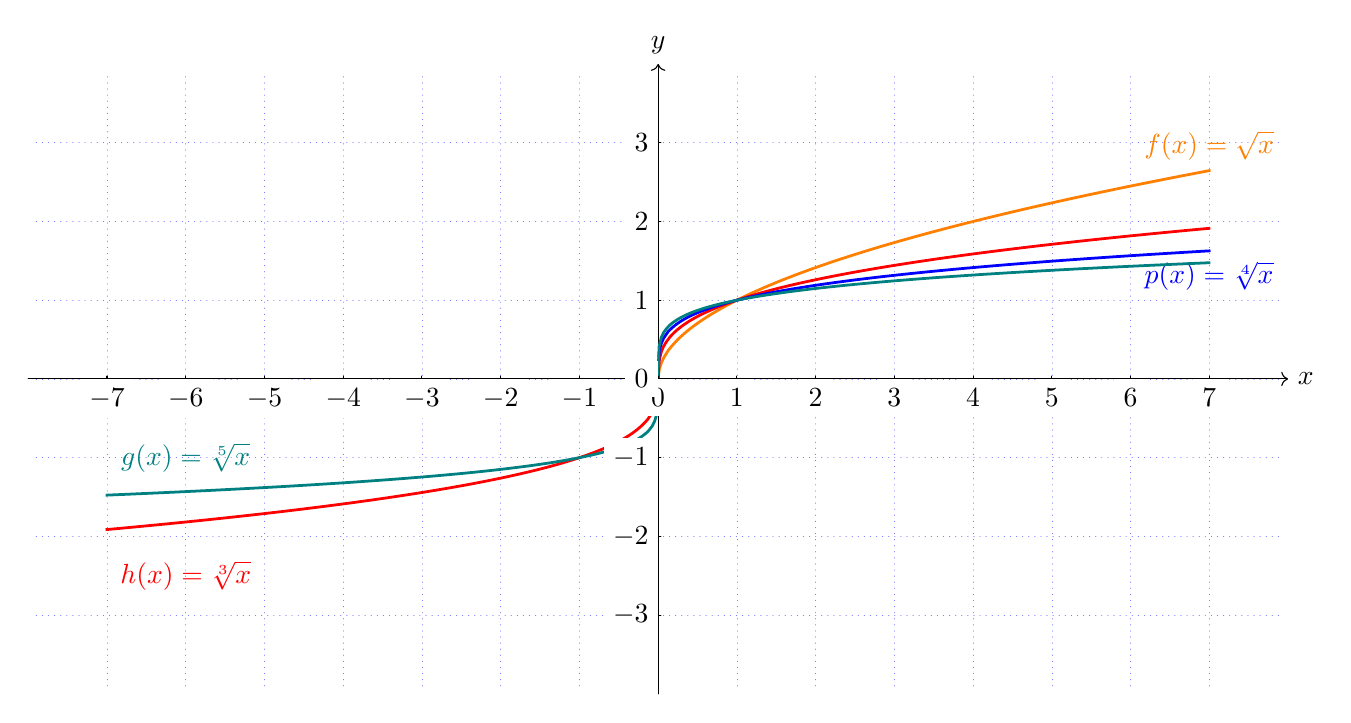
\begin{tikzpicture}[scale=1,cap=round]

% Styles
\tikzstyle{axes}=[]
\tikzstyle help lines=[color=blue!50,very thin,dotted]

% grid
\draw[style=help lines,step=1cm] (-7.9,-3.9) grid (7.9,3.9);

\draw[->] (-8,0) -- (8,0) node[right] {$x$};
\draw[->] (0,-4) -- (0,4) node[above] {$y$};

%\draw[fill,cyan](1,1)circle [radius=0.025];
%FUNCTIEVOORSCHRIFTEN


%------------------
\draw[orange,cap=rect,line width=1, opacity=1, domain=0:7,samples=500] plot (\x, {
	pow(\x,(1/2))  		% <- plaats het functievoorschrift hier
}) node[above,opacity=1]{$f(x)=\sqrt{x}$};

%-------------------------------------------
\draw[red,cap=rect,line width=1, opacity=1, domain=-7:7,samples=500] plot (\x, {
	\x/abs(\x)*abs(\x)^(1/3)% <- plaats het functievoorschrift hier
}) node[opacity=1,pos=0,xshift=-6cm,yshift=-2.5cm]{$h(x)=\sqrt[3]{x}$};

%\draw[red,cap=rect,line width=1, opacity=1, domain=0:7,samples=500] plot (\x, {
%	pow(\x,1/3)  		% <- plaats het functievoorschrift hier
%}) node[opacity=1,left]{$g(x)=x^\frac{1}{3}$};
%-------------------------------------------
\draw[blue,cap=rect,line width=1, opacity=1, domain=0:7,samples=500] plot (\x, {
	pow(\x,(1/4))  		% <- plaats het functievoorschrift hier
}) node[opacity=1,below]{$p(x)=\sqrt[4]{x}$};
%-------------------------------------------

\draw[teal,cap=rect,line width=1, opacity=1, domain=-7:7,samples=500] plot (\x, {
	\x/abs(\x)*abs(\x)^(1/5)% <- plaats het functievoorschrift hier
}) node[opacity=1,pos=0,xshift=-6cm,yshift=-1cm]{$g(x)=\sqrt[5]{x}$};

%\draw[teal,cap=rect,line width=1, opacity=1, domain=0:7,samples=500] plot (\x, {
%	pow(\x,1/5)  		% <- plaats het functievoorschrift hier
%}) node[opacity=1,left]{$g(x)=x^\frac{1}{5}$};
%-------------------------------------------


%legende



%getallen op de x-as en lijntjes   
\foreach \x/\xtext in {-7,-6,-5,-4,-3,-2,-1,0,1,2,3,4,5,6,7}
	\draw[xshift=\x cm] (0pt,1pt) -- (0pt,0pt) node[below,fill=white]
	{$\xtext$};,3
	
%getallen op de y-as en lijntjes  
%BEGIN LUS
\foreach \y/\ytext in {-3,-2,-1,0,1,2,3}
	\draw[yshift=\y cm] (1pt,0pt) -- (0pt,0pt) node[left,fill=white]
	{$\ytext$}; %EINDE LUS



\end{tikzpicture}
\end{center}


\begin{center}
\begin{tikzpicture}[scale=1,cap=round]

% Styles
\tikzstyle{axes}=[]
\tikzstyle help lines=[color=blue!50,very thin,dotted]

% grid
\draw[style=help lines,step=1cm] (-7.9,-1.9) grid (7.9,7.9);

\draw[->] (-8,0) -- (8,0) node[right] {$x$};
\draw[->] (0,-2) -- (0,8) node[above] {$y$};

%\draw[fill,cyan](1,1)circle [radius=0.025];
%FUNCTIEVOORSCHRIFTEN


\draw[blue,cap=rect,line width=1, opacity=1, domain=-7:-2,samples=100] plot (\x, {
	pow(pow(\x,2)-4,1/2)	% <- plaats het functievoorschrift hier	
}) node[opacity=1,above,left]{};
%-------------------------------------------




\draw[blue,cap=rect,line width=1, opacity=1, domain=2:7,samples=100] plot (\x, {
	pow(pow(\x,2)-4,1/2)	% <- plaats het functievoorschrift hier	
}) node[opacity=1,above]{$f(x)=\sqrt{x^2-4}$};
%-------------------------------------------

%legende



%getallen op de x-as en lijntjes   
\foreach \x/\xtext in {-7,-6,-5,-4,-3,-2,-1,0,1,2,3,4,5,6,7}
	\draw[xshift=\x cm] (0pt,1pt) -- (0pt,0pt) node[below,fill=white]
	{$\xtext$};,3
	
%getallen op de y-as en lijntjes  
%BEGIN LUS
\foreach \y/\ytext in {-1,0,1,2,3,4,5,6,7}
	\draw[yshift=\y cm] (1pt,0pt) -- (0pt,0pt) node[left,fill=white]
	{$\ytext$}; %EINDE LUS



\end{tikzpicture}
\end{center}


\tikzsetfigurename{Fig_module_2_1_9_irrat_1}


\begin{center}
\begin{tikzpicture}[scale=1,cap=round]

% Styles
\tikzstyle{axes}=[]
\tikzstyle help lines=[color=blue!50,very thin,dotted]

% grid
\draw[style=help lines,step=1cm] (-2.9,-1.9) grid (7.9,7.9);

\draw[->] (-3,0) -- (8,0) node[right] {$x$};
\draw[->] (0,-2) -- (0,8) node[above] {$y$};

%\draw[fill,cyan](1,1)circle [radius=0.025];
%FUNCTIEVOORSCHRIFTEN


\draw[blue,cap=rect,line width=1, opacity=1, domain=-0.4:5,samples=100] plot (\x, {
	\x+pow(5*\x+2,1/2)-1	% <- plaats het functievoorschrift hier	
}) node[opacity=1,above,left]{$f(x)=x+\sqrt{5x+2}-1
$};
%-------------------------------------------



%legende



%getallen op de x-as en lijntjes   
\foreach \x/\xtext in {-2,-1,0,1,2,3,4,5,6,7}
	\draw[xshift=\x cm] (0pt,1pt) -- (0pt,0pt) node[below,fill=white]
	{$\xtext$};,3
	
%getallen op de y-as en lijntjes  
%BEGIN LUS
\foreach \y/\ytext in {-1,1,2,3,4,5,6,7}
	\draw[yshift=\y cm] (1pt,0pt) -- (0pt,0pt) node[left,fill=white]
	{$\ytext$}; %EINDE LUS



\end{tikzpicture}
\end{center}


\tikzsetfigurename{Fig_module_2_1_9_irrat_2}


\begin{center}
\begin{tikzpicture}[scale=1,cap=round]

% Styles
\tikzstyle{axes}=[]
\tikzstyle help lines=[color=blue!50,very thin,dotted]

% grid
\draw[style=help lines,step=1cm] (-3.9,-5.9) grid (3.9,5.9);

\draw[->] (-4,0) -- (4,0) node[right] {$x$};
\draw[->] (0,-6) -- (0,6) node[above] {$y$};

%\draw[fill,cyan](1,1)circle [radius=0.025];
%FUNCTIEVOORSCHRIFTEN



%\draw[teal,cap=rect,line width=1, opacity=1, domain=-2:2] plot (\x, {
%	pow(\x,2)  		% <- plaats het functievoorschrift hier
%}) node[right,opacity=1]{$h(x)=x^2$};

%\draw[red,cap=rect,line width=1, opacity=1, domain=-1.5:1.5] plot (\x, {
%	pow(\x,4)  		% <- plaats het functievoorschrift hier
%}%) node[opacity=1,above,xshift=-3.5cm]{$p(x)=x^4$};

\draw[blue,cap=rect,line width=1, opacity=1, domain=-2:0.65,samples=100] plot (\x, {
	pow(4-\x*\x,1/2)/(\x-1)	% <- plaats het functievoorschrift hier	
}) node[opacity=1,above,left]{};
%-------------------------------------------

\draw[blue,cap=rect,line width=1, opacity=1, domain=1.3:2,samples=100] plot (\x, {
	pow(4-\x*\x,1/2)/(\x-1)	% <- plaats het functievoorschrift hier	
}) node[opacity=1,above,right,yshift=+3cm]{$f(x)=\frac{\sqrt{4-x^2}}{x-1}
	$};
%-------------------------------------------


%\draw[orange,cap=rect,line width=1, opacity=1, domain=-1.4:1.4] plot (\x, {
%	pow(\x,5)  		% <- plaats het functievoorschrift hier
%}) node[right,opacity=1]{$g(x)=x^5$};



%\draw[cyan,cap=rect,ultra thick, domain=1:2] plot (\x, {\x*\x-1}) node[above, right]{};
%\draw[red,cap=rect, loosely dashed, ultra thick, domain=-2:2] plot (\x, {(\x*\x-1)+0.05}) node[above,yshift=-.7cm, right]{};

%legende



%getallen op de x-as en lijntjes   
\foreach \x/\xtext in {-2,-1,0,1,2}
	\draw[xshift=\x cm] (0pt,1pt) -- (0pt,0pt) node[below,fill=white]
	{$\xtext$};,3
	
%getallen op de y-as en lijntjes  
%BEGIN LUS
\foreach \y/\ytext in {-6,-5,-4,-3,-2,-1,1,2,3,4,5,6}
	\draw[yshift=\y cm] (1pt,0pt) -- (0pt,0pt) node[left,fill=white]
	{$\ytext$}; %EINDE LUS


%%%%%%%%%%%%%%%%%%%%%%%%%%%%%%%
%		MARKERINGEN
%%%%%%%%%%%%%%%%%%%%%%%%%%%%%%%%
%verticale lijn
\draw[line width=1,red, cap=rect,opacity=1] (1,-6) -- (1,6) node[right] {};
%\draw[line width=4,teal, cap=rect,opacity=0.3] (0,0) -- (0,4.2) node[right] {bld $f$ = $\mathbb{R}_0$};
%horizontale lijn
%\draw[line width=4,blue, cap=rect,opacity=0.3] (-1,0) -- (1,0) node[near start,above,xshift=-1.1cm,opacity=1] {maximum in (0,0)};


%\draw[line width=4,blue, cap=rect,opacity=0.3] (1,-4) -- (3,-4) node[below,yshift=-.3cm,opacity=1] {minium in (2,-4)};
\end{tikzpicture}
\end{center}


%		\tikzsetfigurename{Fig_module_2_1_10_exponentiele_functie}
\begin{center}
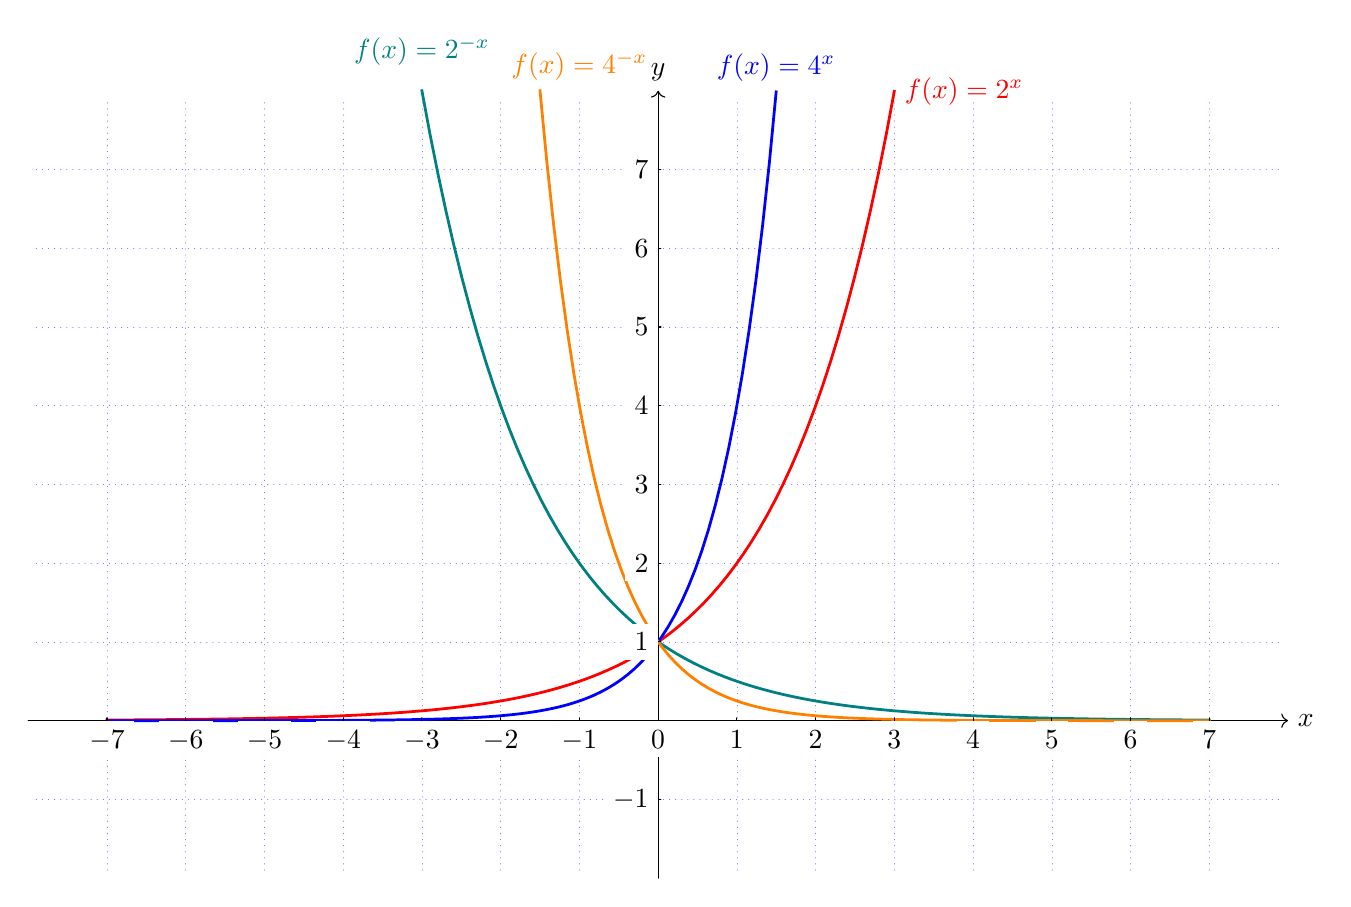
\begin{tikzpicture}[scale=1,cap=round]

% Styles
\tikzstyle{axes}=[]
\tikzstyle help lines=[color=blue!50,very thin,dotted]

% grid
\draw[style=help lines,step=1cm] (-7.9,-1.9) grid (7.9,7.9);

\draw[->] (-8,0) -- (8,0) node[right] {$x$};
\draw[->] (0,-2) -- (0,8) node[above] {$y$};

%\draw[fill,cyan](1,1)circle [radius=0.025];
%FUNCTIEVOORSCHRIFTEN


\draw[red,cap=rect,line width=1, opacity=1, domain=-7:3,samples=100] plot (\x, {
	pow(2,\x)	% <- plaats het functievoorschrift hier	
}) node[opacity=1,above,right]{$f(x)=2^x$};
%-------------------------------------------




\draw[blue,cap=rect,line width=1, opacity=1, domain=-7:1.5,samples=100] plot (\x, {
	pow(4,\x)	% <- plaats het functievoorschrift hier	
}) node[opacity=1,above]{$f(x)=4^x$};
%-------------------------------------------


\draw[teal,cap=rect,line width=1, opacity=1, domain=-3:7,samples=100] plot (\x, {
	pow(2,-\x)	% <- plaats het functievoorschrift hier	
}) node[opacity=1,,pos=0,xshift=-3cm,yshift=+8.5cm]{$f(x)=2^{-x}$};
%-------------------------------------------




\draw[orange,cap=rect,line width=1, opacity=1, domain=-1.5:7,samples=100] plot (\x, {
	pow(4,-\x)	% <- plaats het functievoorschrift hier	
}) node[opacity=1,above,pos=0,xshift=-1cm,yshift=+8cm]{$f(x)=4^{-x}$};
%-------------------------------------------


%legende



%getallen op de x-as en lijntjes   
\foreach \x/\xtext in {-7,-6,-5,-4,-3,-2,-1,0,1,2,3,4,5,6,7}
	\draw[xshift=\x cm] (0pt,1pt) -- (0pt,0pt) node[below,fill=white]
	{$\xtext$};,3
	
%getallen op de y-as en lijntjes  
%BEGIN LUS
\foreach \y/\ytext in {-1,1,2,3,4,5,6,7}
	\draw[yshift=\y cm] (1pt,0pt) -- (0pt,0pt) node[left,fill=white]
	{$\ytext$}; %EINDE LUS



\end{tikzpicture}
\end{center}


%		\tikzsetfigurename{Fig_module_2_1_10_exponentiele_functie_2}

\begin{center}
\begin{tikzpicture}[scale=1,cap=round]

% Styles
\tikzstyle{axes}=[]
\tikzstyle help lines=[color=blue!50,very thin,dotted]

% grid
\draw[style=help lines,step=1cm] (-7.9,-1.9) grid (7.9,7.9);

\draw[->] (-8,0) -- (8,0) node[right] {$x$};
\draw[->] (0,-2) -- (0,8) node[above] {$y$};

%\draw[fill,cyan](1,1)circle [radius=0.025];
%FUNCTIEVOORSCHRIFTEN


\draw[red,cap=rect,line width=1, opacity=1, domain=-7:3,samples=100] plot (\x, {
	pow(2,\x)	% <- plaats het functievoorschrift hier	
}) node[opacity=1,above,right]{$f(x)=2^x$};
%-------------------------------------------



%legende



%getallen op de x-as en lijntjes   
\foreach \x/\xtext in {-7,-6,-5,-4,-3,-2,-1,0,1,2,3,4,5,6,7}
	\draw[xshift=\x cm] (0pt,1pt) -- (0pt,0pt) node[below,fill=white]
	{$\xtext$};,3
	
%getallen op de y-as en lijntjes  
%BEGIN LUS
\foreach \y/\ytext in {-1,1,2,3,4,5,6,7}
	\draw[yshift=\y cm] (1pt,0pt) -- (0pt,0pt) node[left,fill=white]
	{$\ytext$}; %EINDE LUS



\end{tikzpicture}
\end{center}



%TODO polynoombenadering uitrekenen > zie cursus Algebra

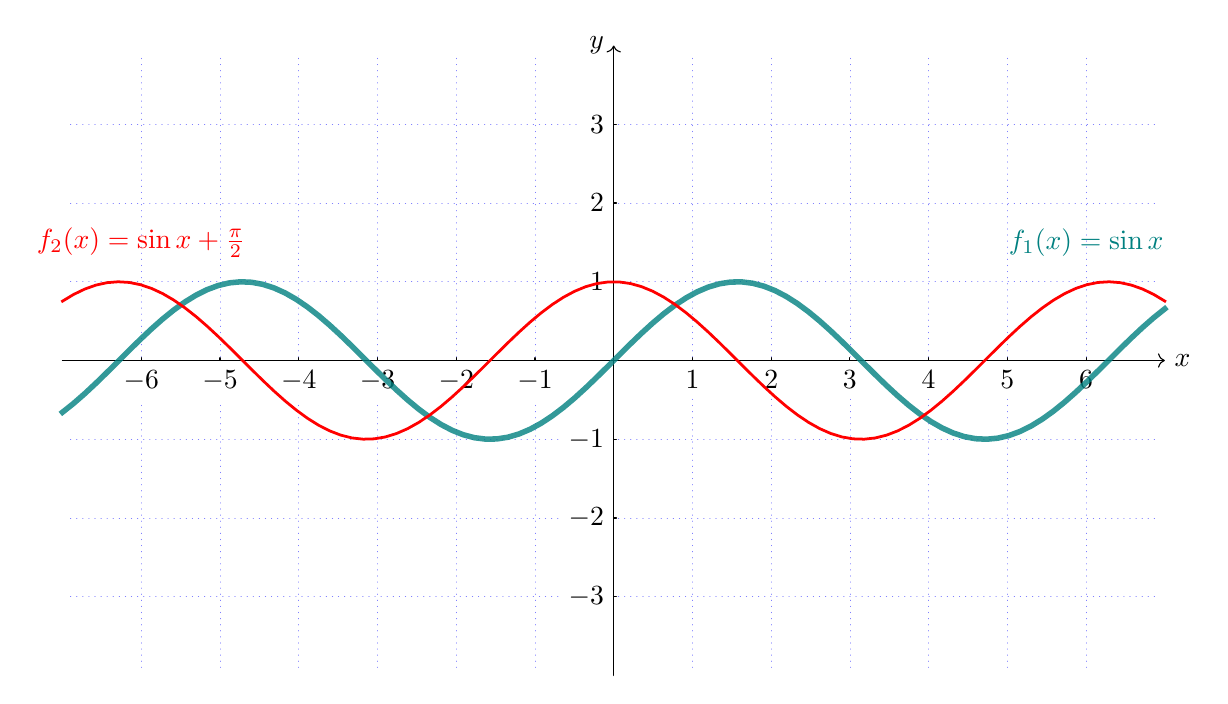
\begin{tikzpicture}[scale=1,cap=round]

% Styles
\tikzstyle{axes}=[]
\tikzstyle help lines=[color=blue!50,very thin,dotted]


%%%%%%%%%%%%%%%%%%%%%%%%%%%%%%%%
%		GRID
%%%%%%%%%%%%%%%%%%%%%%%%%%%%%%%%

\draw[style=help lines,step=1cm] (-6.9,-3.9) grid (6.9,3.9);



%%%%%%%%%%%%%%%%%%%%%%%%%%%%%%%%
%		ASSENSTELSEL
%%%%%%%%%%%%%%%%%%%%%%%%%%%%%%%%

\draw[->] (-7,0) -- (7,0) node[right] {$x$};
\draw[->] (0,-4) -- (0,4) node[left]{$y$};

%\draw[fill,cyan](1,1)circle [radius=0.025];

%\draw[red,cap=rect, loosely dashed, ultra thick, domain=-2:2] plot (\x, {(\x*\x-1)+0.05}) node[above,yshift=-.7cm, right]{};

%%%%%%%%%%%%%%%%%%%%%%%%%%%%%%%%
%legende
%%%%%%%%%%%%%%%%%%%%%%%%%%%%%%%%
%\tkzDefPoint(0.5,3.5){A}
%\tkzDefPoint(1,3.5){B}
%\tkzLabelPoint[right,xshift=+0.1cm](B){${\color{cyan}f(x)=|x^2-1|}$}
%\tkzDrawSegment[cyan,ultra thick](A,B)

%\tkzDefPoint(0.5,3.2){C}
%\tkzDefPoint(1,3.2){D}
%\tkzLabelPoint[right,xshift=+0.1cm](D){${\color{red}e(x)=x^2-1}$}
%\tkzDrawSegment[red,cap=rect, loosely dashed, ultra thick](C,D)


%%%%%%%%%%%%%%%%%%%%%%%%%%%%%%%%
%getallen op de x-as en lijntjes
%%%%%%%%%%%%%%%%%%%%%%%%%%%%%%%%   
\foreach \x/\xtext in {-6,-5,-4,-3,-2,-1,1,2,3,4,5,6}
	\draw[xshift=\x cm] (0pt,1pt) -- (0pt,0pt) node[below,fill=white]
	{$\xtext$};,3
	
%getallen op de y-as en lijntjes  
%BEGIN LUS
\foreach \y/\ytext in {-3,-2,-1,1,2,3}
	\draw[yshift=\y cm] (1pt,0pt) -- (0pt,0pt) node[left,fill=white]
	{$\ytext$}; %EINDE LUS



%%%%%%%%%%%%%%%%%%%%%%%%%%%%%%%%
%		GRAFIEKEN
%%%%%%%%%%%%%%%%%%%%%%%%%%%%%%%%


\draw[teal,cap=rect,line width=2, opacity=0.8, domain=-7:7,samples=100] plot (\x, {
	sin(\x r)	% <- plaats het functievoorschrift hier	
}) node[opacity=1,,pos=0,xshift=+6cm,yshift=+1.5cm]{$f_1(x)=\sin{x}$};
%-------------------------------------------
\draw[red,cap=rect,line width=1, opacity=1, domain=-7:7,samples=100] plot (\x, {
	sin((\x +pi/2) r)	% <- plaats het functievoorschrift hier	
}) node[opacity=1,,pos=0,xshift=-6cm,yshift=+1.5cm]{$f_2(x)=\sin{x+\frac{\pi}{2}}$};
%-------------------------------------------



%\draw[cyan,cap=rect,thick, domain=-6:6] plot (\x, \x) node[above, right]{${\color{cyan}y=x}$};v

%\draw[cyan,cap=rect,ultra thick, domain=-6:1.75] plot (\x, {(\x-2)^(-1)}) node[above,right]{};


%\draw[cyan,cap=rect,ultra thick, domain=2.25:6] plot (\x, {(\x-2)^(-1)}) node[above,yshift=+0.5cm,left]{$\color{cyan} y=\frac{1}{x-2}$};


%\draw[cyan,cap=rect,ultra thick, domain=-7:1.9] plot (\x, {exp{\x}}) node[above, right]{${\color{cyan}y=\exp{x}}$};

%%%%%%%%%%%%%%%%%%%%%%%%%%%%%%%%
%		MARKERINGEN
%%%%%%%%%%%%%%%%%%%%%%%%%%%%%%%%
%verticale lijn
%\draw[-o,line width=4,teal, cap=rect,opacity=0.3] (0,-4) -- (0,0.25) node[right] {};
%\draw[line width=4,teal, cap=rect,opacity=0.3] (0,0) -- (0,4.2) node[right] {bld $f$ = $\mathbb{R}_0$};
%horizontale lijn
%\draw[arrows=-o,line width=4,blue, cap=rect,opacity=0.3] (-7,0) -- (2.25,0) node[right] {};
%\draw[line width=4,blue, cap=rect,opacity=0.3] (2.25,0) -- (7,0) node[below,yshift=-0.3cm] {dom$f$ = $\mathbb{R}  \setminus 2 $};
 
\end{tikzpicture}

		\tikzsetfigurename{Fig_module_2_1_15_verschuiven_en_verschalen_2}



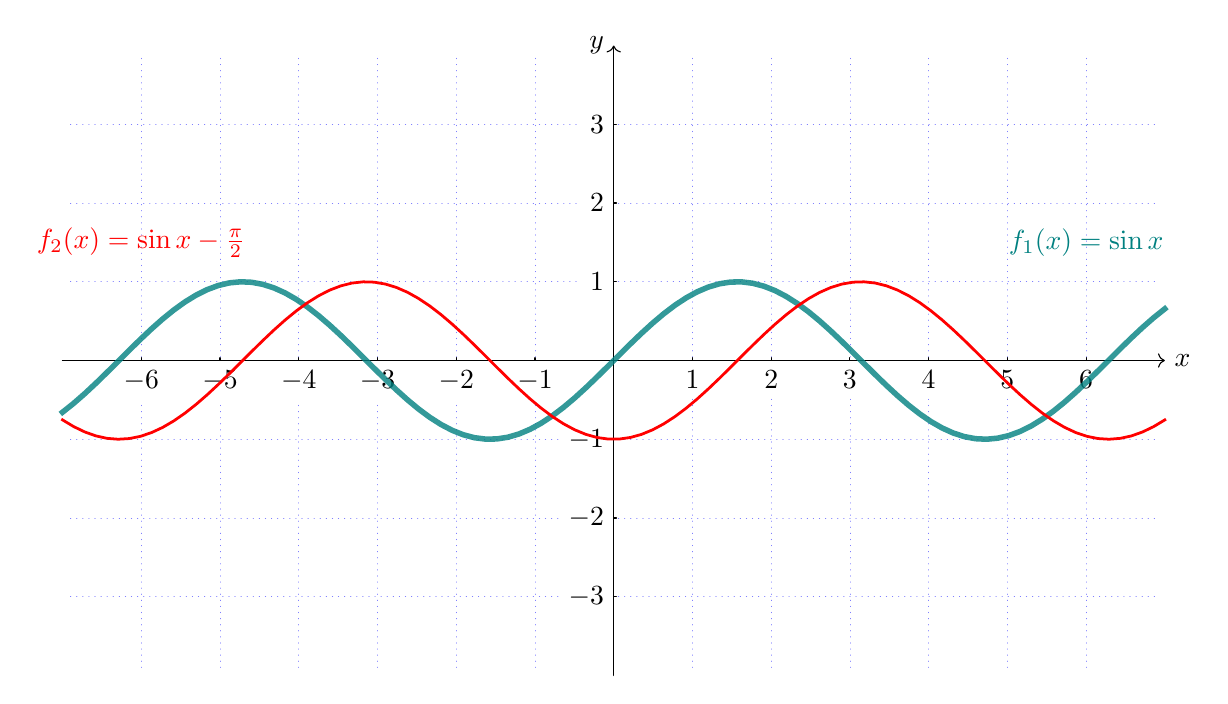
\begin{tikzpicture}[scale=1,cap=round]

% Styles
\tikzstyle{axes}=[]
\tikzstyle help lines=[color=blue!50,very thin,dotted]


%%%%%%%%%%%%%%%%%%%%%%%%%%%%%%%%
%		GRID
%%%%%%%%%%%%%%%%%%%%%%%%%%%%%%%%

\draw[style=help lines,step=1cm] (-6.9,-3.9) grid (6.9,3.9);



%%%%%%%%%%%%%%%%%%%%%%%%%%%%%%%%
%		ASSENSTELSEL
%%%%%%%%%%%%%%%%%%%%%%%%%%%%%%%%

\draw[->] (-7,0) -- (7,0) node[right] {$x$};
\draw[->] (0,-4) -- (0,4) node[left]{$y$};

%\draw[fill,cyan](1,1)circle [radius=0.025];

%\draw[red,cap=rect, loosely dashed, ultra thick, domain=-2:2] plot (\x, {(\x*\x-1)+0.05}) node[above,yshift=-.7cm, right]{};

%%%%%%%%%%%%%%%%%%%%%%%%%%%%%%%%
%legende
%%%%%%%%%%%%%%%%%%%%%%%%%%%%%%%%
%\tkzDefPoint(0.5,3.5){A}
%\tkzDefPoint(1,3.5){B}
%\tkzLabelPoint[right,xshift=+0.1cm](B){${\color{cyan}f(x)=|x^2-1|}$}
%\tkzDrawSegment[cyan,ultra thick](A,B)

%\tkzDefPoint(0.5,3.2){C}
%\tkzDefPoint(1,3.2){D}
%\tkzLabelPoint[right,xshift=+0.1cm](D){${\color{red}e(x)=x^2-1}$}
%\tkzDrawSegment[red,cap=rect, loosely dashed, ultra thick](C,D)


%%%%%%%%%%%%%%%%%%%%%%%%%%%%%%%%
%getallen op de x-as en lijntjes
%%%%%%%%%%%%%%%%%%%%%%%%%%%%%%%%   
\foreach \x/\xtext in {-6,-5,-4,-3,-2,-1,1,2,3,4,5,6}
	\draw[xshift=\x cm] (0pt,1pt) -- (0pt,0pt) node[below,fill=white]
	{$\xtext$};,3
	
%getallen op de y-as en lijntjes  
%BEGIN LUS
\foreach \y/\ytext in {-3,-2,-1,1,2,3}
	\draw[yshift=\y cm] (1pt,0pt) -- (0pt,0pt) node[left,fill=white]
	{$\ytext$}; %EINDE LUS



%%%%%%%%%%%%%%%%%%%%%%%%%%%%%%%%
%		GRAFIEKEN
%%%%%%%%%%%%%%%%%%%%%%%%%%%%%%%%


\draw[teal,cap=rect,line width=2, opacity=0.8, domain=-7:7,samples=100] plot (\x, {
	sin(\x r)	% <- plaats het functievoorschrift hier	
}) node[opacity=1,,pos=0,xshift=+6cm,yshift=+1.5cm]{$f_1(x)=\sin{x}$};
%-------------------------------------------
\draw[red,cap=rect,line width=1, opacity=1, domain=-7:7,samples=100] plot (\x, {
	sin((\x -pi/2) r)	% <- plaats het functievoorschrift hier	
}) node[opacity=1,,pos=0,xshift=-6cm,yshift=+1.5cm]{$f_2(x)=\sin{x-\frac{\pi}{2}}$};
%-------------------------------------------



%\draw[cyan,cap=rect,thick, domain=-6:6] plot (\x, \x) node[above, right]{${\color{cyan}y=x}$};v

%\draw[cyan,cap=rect,ultra thick, domain=-6:1.75] plot (\x, {(\x-2)^(-1)}) node[above,right]{};


%\draw[cyan,cap=rect,ultra thick, domain=2.25:6] plot (\x, {(\x-2)^(-1)}) node[above,yshift=+0.5cm,left]{$\color{cyan} y=\frac{1}{x-2}$};


%\draw[cyan,cap=rect,ultra thick, domain=-7:1.9] plot (\x, {exp{\x}}) node[above, right]{${\color{cyan}y=\exp{x}}$};

%%%%%%%%%%%%%%%%%%%%%%%%%%%%%%%%
%		MARKERINGEN
%%%%%%%%%%%%%%%%%%%%%%%%%%%%%%%%
%verticale lijn
%\draw[-o,line width=4,teal, cap=rect,opacity=0.3] (0,-4) -- (0,0.25) node[right] {};
%\draw[line width=4,teal, cap=rect,opacity=0.3] (0,0) -- (0,4.2) node[right] {bld $f$ = $\mathbb{R}_0$};
%horizontale lijn
%\draw[arrows=-o,line width=4,blue, cap=rect,opacity=0.3] (-7,0) -- (2.25,0) node[right] {};
%\draw[line width=4,blue, cap=rect,opacity=0.3] (2.25,0) -- (7,0) node[below,yshift=-0.3cm] {dom$f$ = $\mathbb{R}  \setminus 2 $};
 
\end{tikzpicture}


%TODO polynoombenadering uitrekenen > zie cursus Algebra

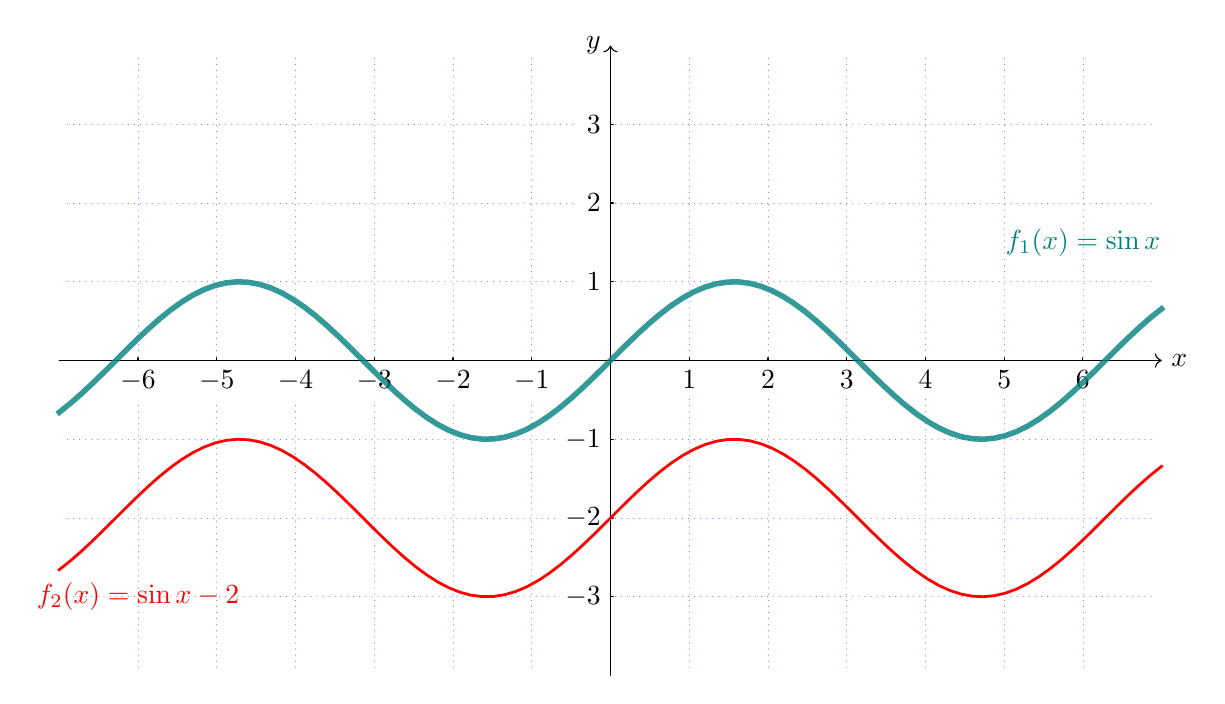
\begin{tikzpicture}[scale=1,cap=round]

% Styles
\tikzstyle{axes}=[]
\tikzstyle help lines=[color=blue!50,very thin,dotted]


%%%%%%%%%%%%%%%%%%%%%%%%%%%%%%%%
%		GRID
%%%%%%%%%%%%%%%%%%%%%%%%%%%%%%%%

\draw[style=help lines,step=1cm] (-6.9,-3.9) grid (6.9,3.9);



%%%%%%%%%%%%%%%%%%%%%%%%%%%%%%%%
%		ASSENSTELSEL
%%%%%%%%%%%%%%%%%%%%%%%%%%%%%%%%

\draw[->] (-7,0) -- (7,0) node[right] {$x$};
\draw[->] (0,-4) -- (0,4) node[left]{$y$};

%\draw[fill,cyan](1,1)circle [radius=0.025];

%\draw[red,cap=rect, loosely dashed, ultra thick, domain=-2:2] plot (\x, {(\x*\x-1)+0.05}) node[above,yshift=-.7cm, right]{};

%%%%%%%%%%%%%%%%%%%%%%%%%%%%%%%%
%legende
%%%%%%%%%%%%%%%%%%%%%%%%%%%%%%%%
%\tkzDefPoint(0.5,3.5){A}
%\tkzDefPoint(1,3.5){B}
%\tkzLabelPoint[right,xshift=+0.1cm](B){${\color{cyan}f(x)=|x^2-1|}$}
%\tkzDrawSegment[cyan,ultra thick](A,B)

%\tkzDefPoint(0.5,3.2){C}
%\tkzDefPoint(1,3.2){D}
%\tkzLabelPoint[right,xshift=+0.1cm](D){${\color{red}e(x)=x^2-1}$}
%\tkzDrawSegment[red,cap=rect, loosely dashed, ultra thick](C,D)


%%%%%%%%%%%%%%%%%%%%%%%%%%%%%%%%
%getallen op de x-as en lijntjes
%%%%%%%%%%%%%%%%%%%%%%%%%%%%%%%%   
\foreach \x/\xtext in {-6,-5,-4,-3,-2,-1,1,2,3,4,5,6}
	\draw[xshift=\x cm] (0pt,1pt) -- (0pt,0pt) node[below,fill=white]
	{$\xtext$};,3
	
%getallen op de y-as en lijntjes  
%BEGIN LUS
\foreach \y/\ytext in {-3,-2,-1,1,2,3}
	\draw[yshift=\y cm] (1pt,0pt) -- (0pt,0pt) node[left,fill=white]
	{$\ytext$}; %EINDE LUS



%%%%%%%%%%%%%%%%%%%%%%%%%%%%%%%%
%		GRAFIEKEN
%%%%%%%%%%%%%%%%%%%%%%%%%%%%%%%%


\draw[teal,cap=rect,line width=2, opacity=0.8, domain=-7:7,samples=100] plot (\x, {
	sin(\x r)	% <- plaats het functievoorschrift hier	
}) node[opacity=1,,pos=0,xshift=+6cm,yshift=+1.5cm]{$f_1(x)=\sin{x}$};
%-------------------------------------------
\draw[red,cap=rect,line width=1, opacity=1, domain=-7:7,samples=100] plot (\x, {
	(sin((\x r))-2	% <- plaats het functievoorschrift hier	
}) node[opacity=1,,pos=0,xshift=-6cm,yshift=-3cm]{$f_2(x)=\sin{x}-2$};
%-------------------------------------------



%\draw[cyan,cap=rect,thick, domain=-6:6] plot (\x, \x) node[above, right]{${\color{cyan}y=x}$};v

%\draw[cyan,cap=rect,ultra thick, domain=-6:1.75] plot (\x, {(\x-2)^(-1)}) node[above,right]{};


%\draw[cyan,cap=rect,ultra thick, domain=2.25:6] plot (\x, {(\x-2)^(-1)}) node[above,yshift=+0.5cm,left]{$\color{cyan} y=\frac{1}{x-2}$};


%\draw[cyan,cap=rect,ultra thick, domain=-7:1.9] plot (\x, {exp{\x}}) node[above, right]{${\color{cyan}y=\exp{x}}$};

%%%%%%%%%%%%%%%%%%%%%%%%%%%%%%%%
%		MARKERINGEN
%%%%%%%%%%%%%%%%%%%%%%%%%%%%%%%%
%verticale lijn
%\draw[-o,line width=4,teal, cap=rect,opacity=0.3] (0,-4) -- (0,0.25) node[right] {};
%\draw[line width=4,teal, cap=rect,opacity=0.3] (0,0) -- (0,4.2) node[right] {bld $f$ = $\mathbb{R}_0$};
%horizontale lijn
%\draw[arrows=-o,line width=4,blue, cap=rect,opacity=0.3] (-7,0) -- (2.25,0) node[right] {};
%\draw[line width=4,blue, cap=rect,opacity=0.3] (2.25,0) -- (7,0) node[below,yshift=-0.3cm] {dom$f$ = $\mathbb{R}  \setminus 2 $};
 
\end{tikzpicture}


%TODO polynoombenadering uitrekenen > zie cursus Algebra

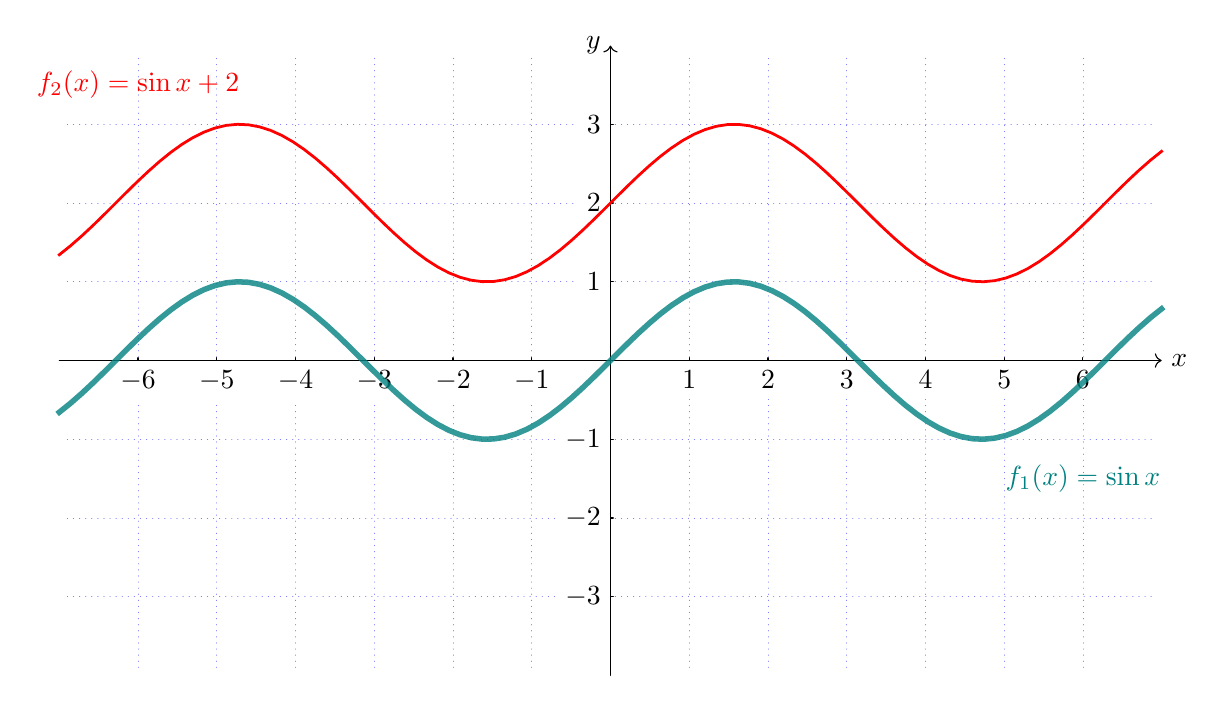
\begin{tikzpicture}[scale=1,cap=round]

% Styles
\tikzstyle{axes}=[]
\tikzstyle help lines=[color=blue!50,very thin,dotted]


%%%%%%%%%%%%%%%%%%%%%%%%%%%%%%%%
%		GRID
%%%%%%%%%%%%%%%%%%%%%%%%%%%%%%%%

\draw[style=help lines,step=1cm] (-6.9,-3.9) grid (6.9,3.9);



%%%%%%%%%%%%%%%%%%%%%%%%%%%%%%%%
%		ASSENSTELSEL
%%%%%%%%%%%%%%%%%%%%%%%%%%%%%%%%

\draw[->] (-7,0) -- (7,0) node[right] {$x$};
\draw[->] (0,-4) -- (0,4) node[left]{$y$};

%\draw[fill,cyan](1,1)circle [radius=0.025];

%\draw[red,cap=rect, loosely dashed, ultra thick, domain=-2:2] plot (\x, {(\x*\x-1)+0.05}) node[above,yshift=-.7cm, right]{};

%%%%%%%%%%%%%%%%%%%%%%%%%%%%%%%%
%legende
%%%%%%%%%%%%%%%%%%%%%%%%%%%%%%%%
%\tkzDefPoint(0.5,3.5){A}
%\tkzDefPoint(1,3.5){B}
%\tkzLabelPoint[right,xshift=+0.1cm](B){${\color{cyan}f(x)=|x^2-1|}$}
%\tkzDrawSegment[cyan,ultra thick](A,B)

%\tkzDefPoint(0.5,3.2){C}
%\tkzDefPoint(1,3.2){D}
%\tkzLabelPoint[right,xshift=+0.1cm](D){${\color{red}e(x)=x^2-1}$}
%\tkzDrawSegment[red,cap=rect, loosely dashed, ultra thick](C,D)


%%%%%%%%%%%%%%%%%%%%%%%%%%%%%%%%
%getallen op de x-as en lijntjes
%%%%%%%%%%%%%%%%%%%%%%%%%%%%%%%%   
\foreach \x/\xtext in {-6,-5,-4,-3,-2,-1,1,2,3,4,5,6}
	\draw[xshift=\x cm] (0pt,1pt) -- (0pt,0pt) node[below,fill=white]
	{$\xtext$};,3
	
%getallen op de y-as en lijntjes  
%BEGIN LUS
\foreach \y/\ytext in {-3,-2,-1,1,2,3}
	\draw[yshift=\y cm] (1pt,0pt) -- (0pt,0pt) node[left,fill=white]
	{$\ytext$}; %EINDE LUS



%%%%%%%%%%%%%%%%%%%%%%%%%%%%%%%%
%		GRAFIEKEN
%%%%%%%%%%%%%%%%%%%%%%%%%%%%%%%%


\draw[teal,cap=rect,line width=2, opacity=0.8, domain=-7:7,samples=100] plot (\x, {
	sin(\x r)	% <- plaats het functievoorschrift hier	
}) node[opacity=1,,pos=0,xshift=+6cm,yshift=-1.5cm]{$f_1(x)=\sin{x}$};
%-------------------------------------------
\draw[red,cap=rect,line width=1, opacity=1, domain=-7:7,samples=100] plot (\x, {
	(sin((\x r))+2	% <- plaats het functievoorschrift hier	
}) node[opacity=1,,pos=0,xshift=-6cm,yshift=+3.5cm]{$f_2(x)=\sin{x}+2$};
%-------------------------------------------



%\draw[cyan,cap=rect,thick, domain=-6:6] plot (\x, \x) node[above, right]{${\color{cyan}y=x}$};v

%\draw[cyan,cap=rect,ultra thick, domain=-6:1.75] plot (\x, {(\x-2)^(-1)}) node[above,right]{};


%\draw[cyan,cap=rect,ultra thick, domain=2.25:6] plot (\x, {(\x-2)^(-1)}) node[above,yshift=+0.5cm,left]{$\color{cyan} y=\frac{1}{x-2}$};


%\draw[cyan,cap=rect,ultra thick, domain=-7:1.9] plot (\x, {exp{\x}}) node[above, right]{${\color{cyan}y=\exp{x}}$};

%%%%%%%%%%%%%%%%%%%%%%%%%%%%%%%%
%		MARKERINGEN
%%%%%%%%%%%%%%%%%%%%%%%%%%%%%%%%
%verticale lijn
%\draw[-o,line width=4,teal, cap=rect,opacity=0.3] (0,-4) -- (0,0.25) node[right] {};
%\draw[line width=4,teal, cap=rect,opacity=0.3] (0,0) -- (0,4.2) node[right] {bld $f$ = $\mathbb{R}_0$};
%horizontale lijn
%\draw[arrows=-o,line width=4,blue, cap=rect,opacity=0.3] (-7,0) -- (2.25,0) node[right] {};
%\draw[line width=4,blue, cap=rect,opacity=0.3] (2.25,0) -- (7,0) node[below,yshift=-0.3cm] {dom$f$ = $\mathbb{R}  \setminus 2 $};
 
\end{tikzpicture}

		\tikzsetfigurename{Fig_module_2_1_15_verschuiven_en_verschalen_5}


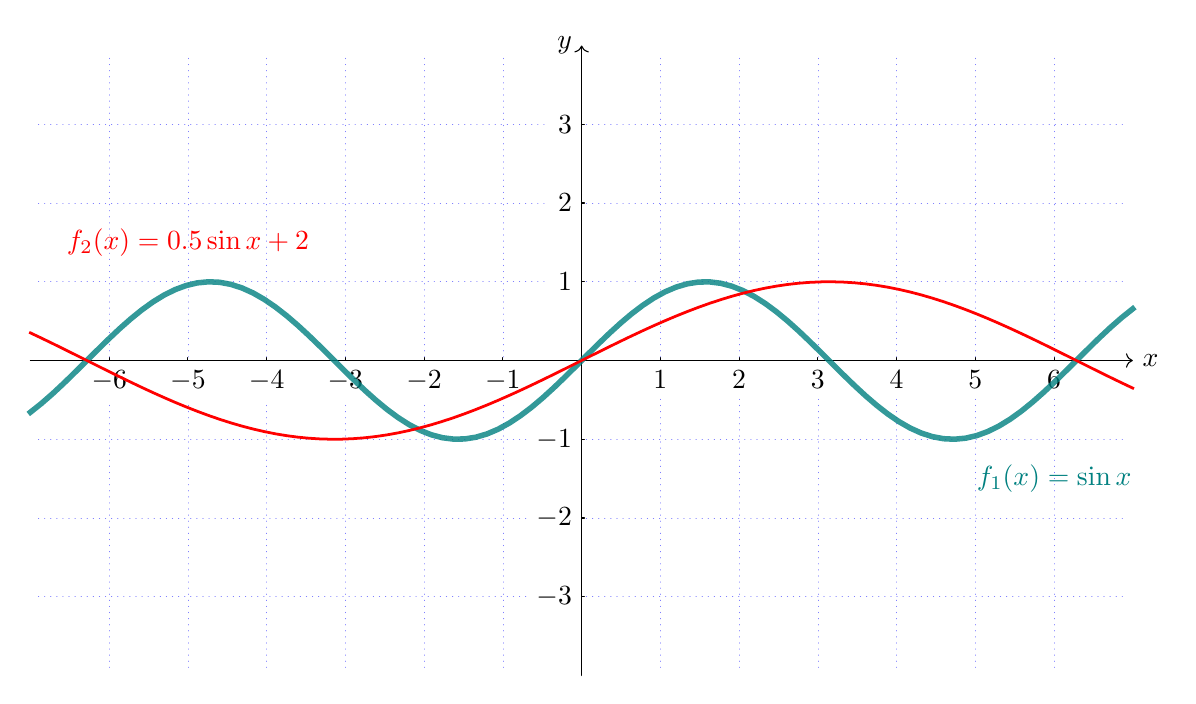
\begin{tikzpicture}[scale=1,cap=round]

% Styles
\tikzstyle{axes}=[]
\tikzstyle help lines=[color=blue!50,very thin,dotted]


%%%%%%%%%%%%%%%%%%%%%%%%%%%%%%%%
%		GRID
%%%%%%%%%%%%%%%%%%%%%%%%%%%%%%%%

\draw[style=help lines,step=1cm] (-6.9,-3.9) grid (6.9,3.9);



%%%%%%%%%%%%%%%%%%%%%%%%%%%%%%%%
%		ASSENSTELSEL
%%%%%%%%%%%%%%%%%%%%%%%%%%%%%%%%

\draw[->] (-7,0) -- (7,0) node[right] {$x$};
\draw[->] (0,-4) -- (0,4) node[left]{$y$};

%\draw[fill,cyan](1,1)circle [radius=0.025];

%\draw[red,cap=rect, loosely dashed, ultra thick, domain=-2:2] plot (\x, {(\x*\x-1)+0.05}) node[above,yshift=-.7cm, right]{};

%%%%%%%%%%%%%%%%%%%%%%%%%%%%%%%%
%legende
%%%%%%%%%%%%%%%%%%%%%%%%%%%%%%%%
%\tkzDefPoint(0.5,3.5){A}
%\tkzDefPoint(1,3.5){B}
%\tkzLabelPoint[right,xshift=+0.1cm](B){${\color{cyan}f(x)=|x^2-1|}$}
%\tkzDrawSegment[cyan,ultra thick](A,B)

%\tkzDefPoint(0.5,3.2){C}
%\tkzDefPoint(1,3.2){D}
%\tkzLabelPoint[right,xshift=+0.1cm](D){${\color{red}e(x)=x^2-1}$}
%\tkzDrawSegment[red,cap=rect, loosely dashed, ultra thick](C,D)


%%%%%%%%%%%%%%%%%%%%%%%%%%%%%%%%
%getallen op de x-as en lijntjes
%%%%%%%%%%%%%%%%%%%%%%%%%%%%%%%%   
\foreach \x/\xtext in {-6,-5,-4,-3,-2,-1,1,2,3,4,5,6}
	\draw[xshift=\x cm] (0pt,1pt) -- (0pt,0pt) node[below,fill=white]
	{$\xtext$};,3
	
%getallen op de y-as en lijntjes  
%BEGIN LUS
\foreach \y/\ytext in {-3,-2,-1,1,2,3}
	\draw[yshift=\y cm] (1pt,0pt) -- (0pt,0pt) node[left,fill=white]
	{$\ytext$}; %EINDE LUS



%%%%%%%%%%%%%%%%%%%%%%%%%%%%%%%%
%		GRAFIEKEN
%%%%%%%%%%%%%%%%%%%%%%%%%%%%%%%%


\draw[teal,cap=rect,line width=2, opacity=0.8, domain=-7:7,samples=100] plot (\x, {
	sin(\x r)	% <- plaats het functievoorschrift hier	
}) node[opacity=1,,pos=0,xshift=+6cm,yshift=-1.5cm]{$f_1(x)=\sin{x}$};
%-------------------------------------------
\draw[red,cap=rect,line width=1, opacity=1, domain=-7:7,samples=100] plot (\x, {
	(sin(0.5*(\x r))	% <- plaats het functievoorschrift hier	
}) node[opacity=1,,pos=0,xshift=-5cm,yshift=+1.5cm]{$f_2(x)=0.5\sin{x}+2$};
%-------------------------------------------



%\draw[cyan,cap=rect,thick, domain=-6:6] plot (\x, \x) node[above, right]{${\color{cyan}y=x}$};v

%\draw[cyan,cap=rect,ultra thick, domain=-6:1.75] plot (\x, {(\x-2)^(-1)}) node[above,right]{};


%\draw[cyan,cap=rect,ultra thick, domain=2.25:6] plot (\x, {(\x-2)^(-1)}) node[above,yshift=+0.5cm,left]{$\color{cyan} y=\frac{1}{x-2}$};


%\draw[cyan,cap=rect,ultra thick, domain=-7:1.9] plot (\x, {exp{\x}}) node[above, right]{${\color{cyan}y=\exp{x}}$};

%%%%%%%%%%%%%%%%%%%%%%%%%%%%%%%%
%		MARKERINGEN
%%%%%%%%%%%%%%%%%%%%%%%%%%%%%%%%
%verticale lijn
%\draw[-o,line width=4,teal, cap=rect,opacity=0.3] (0,-4) -- (0,0.25) node[right] {};
%\draw[line width=4,teal, cap=rect,opacity=0.3] (0,0) -- (0,4.2) node[right] {bld $f$ = $\mathbb{R}_0$};
%horizontale lijn
%\draw[arrows=-o,line width=4,blue, cap=rect,opacity=0.3] (-7,0) -- (2.25,0) node[right] {};
%\draw[line width=4,blue, cap=rect,opacity=0.3] (2.25,0) -- (7,0) node[below,yshift=-0.3cm] {dom$f$ = $\mathbb{R}  \setminus 2 $};
 
\end{tikzpicture}

		\tikzsetfigurename{Fig_module_2_1_15_verschuiven_en_verschalen_6}


\begin{tikzpicture}[scale=1,cap=round]

% Styles
\tikzstyle{axes}=[]
\tikzstyle help lines=[color=blue!50,very thin,dotted]


%%%%%%%%%%%%%%%%%%%%%%%%%%%%%%%%
%		GRID
%%%%%%%%%%%%%%%%%%%%%%%%%%%%%%%%

\draw[style=help lines,step=1cm] (-6.9,-3.9) grid (6.9,3.9);



%%%%%%%%%%%%%%%%%%%%%%%%%%%%%%%%
%		ASSENSTELSEL
%%%%%%%%%%%%%%%%%%%%%%%%%%%%%%%%

\draw[->] (-7,0) -- (7,0) node[right] {$x$};
\draw[->] (0,-4) -- (0,4) node[left]{$y$};

%\draw[fill,cyan](1,1)circle [radius=0.025];

%\draw[red,cap=rect, loosely dashed, ultra thick, domain=-2:2] plot (\x, {(\x*\x-1)+0.05}) node[above,yshift=-.7cm, right]{};

%%%%%%%%%%%%%%%%%%%%%%%%%%%%%%%%
%legende
%%%%%%%%%%%%%%%%%%%%%%%%%%%%%%%%
%\tkzDefPoint(0.5,3.5){A}
%\tkzDefPoint(1,3.5){B}
%\tkzLabelPoint[right,xshift=+0.1cm](B){${\color{cyan}f(x)=|x^2-1|}$}
%\tkzDrawSegment[cyan,ultra thick](A,B)

%\tkzDefPoint(0.5,3.2){C}
%\tkzDefPoint(1,3.2){D}
%\tkzLabelPoint[right,xshift=+0.1cm](D){${\color{red}e(x)=x^2-1}$}
%\tkzDrawSegment[red,cap=rect, loosely dashed, ultra thick](C,D)


%%%%%%%%%%%%%%%%%%%%%%%%%%%%%%%%
%getallen op de x-as en lijntjes
%%%%%%%%%%%%%%%%%%%%%%%%%%%%%%%%   
\foreach \x/\xtext in {-6,-5,-4,-3,-2,-1,1,2,3,4,5,6}
	\draw[xshift=\x cm] (0pt,1pt) -- (0pt,0pt) node[below,fill=white]
	{$\xtext$};,3
	
%getallen op de y-as en lijntjes  
%BEGIN LUS
\foreach \y/\ytext in {-3,-2,-1,1,2,3}
	\draw[yshift=\y cm] (1pt,0pt) -- (0pt,0pt) node[left,fill=white]
	{$\ytext$}; %EINDE LUS



%%%%%%%%%%%%%%%%%%%%%%%%%%%%%%%%
%		GRAFIEKEN
%%%%%%%%%%%%%%%%%%%%%%%%%%%%%%%%


\draw[teal,cap=rect,line width=2, opacity=0.8, domain=-7:7,samples=100] plot (\x, {
	sin(\x r)	% <- plaats het functievoorschrift hier	
}) node[opacity=1,,pos=0,xshift=+6cm,yshift=-1.5cm]{$f_1(x)=\sin{x}$};
%-------------------------------------------
\draw[red,cap=rect,line width=1, opacity=1, domain=-7:7,samples=100] plot (\x, {
	(sin(2*(\x r))	% <- plaats het functievoorschrift hier	
}) node[opacity=1,,pos=0,xshift=-5.cm,yshift=+1.5cm]{$f_2(x)=0.3\sin{x}+2$};
%-------------------------------------------



%\draw[cyan,cap=rect,thick, domain=-6:6] plot (\x, \x) node[above, right]{${\color{cyan}y=x}$};v

%\draw[cyan,cap=rect,ultra thick, domain=-6:1.75] plot (\x, {(\x-2)^(-1)}) node[above,right]{};


%\draw[cyan,cap=rect,ultra thick, domain=2.25:6] plot (\x, {(\x-2)^(-1)}) node[above,yshift=+0.5cm,left]{$\color{cyan} y=\frac{1}{x-2}$};


%\draw[cyan,cap=rect,ultra thick, domain=-7:1.9] plot (\x, {exp{\x}}) node[above, right]{${\color{cyan}y=\exp{x}}$};

%%%%%%%%%%%%%%%%%%%%%%%%%%%%%%%%
%		MARKERINGEN
%%%%%%%%%%%%%%%%%%%%%%%%%%%%%%%%
%verticale lijn
%\draw[-o,line width=4,teal, cap=rect,opacity=0.3] (0,-4) -- (0,0.25) node[right] {};
%\draw[line width=4,teal, cap=rect,opacity=0.3] (0,0) -- (0,4.2) node[right] {bld $f$ = $\mathbb{R}_0$};
%horizontale lijn
%\draw[arrows=-o,line width=4,blue, cap=rect,opacity=0.3] (-7,0) -- (2.25,0) node[right] {};
%\draw[line width=4,blue, cap=rect,opacity=0.3] (2.25,0) -- (7,0) node[below,yshift=-0.3cm] {dom$f$ = $\mathbb{R}  \setminus 2 $};
 
\end{tikzpicture}


%TODO polynoombenadering uitrekenen > zie cursus Algebra

\begin{tikzpicture}[scale=1,cap=round]

% Styles
\tikzstyle{axes}=[]
\tikzstyle help lines=[color=blue!50,very thin,dotted]


%%%%%%%%%%%%%%%%%%%%%%%%%%%%%%%%
%		GRID
%%%%%%%%%%%%%%%%%%%%%%%%%%%%%%%%

\draw[style=help lines,step=1cm] (-6.9,-3.9) grid (6.9,3.9);



%%%%%%%%%%%%%%%%%%%%%%%%%%%%%%%%
%		ASSENSTELSEL
%%%%%%%%%%%%%%%%%%%%%%%%%%%%%%%%

\draw[->] (-7,0) -- (7,0) node[right] {$x$};
\draw[->] (0,-4) -- (0,4) node[left]{$y$};

%\draw[fill,cyan](1,1)circle [radius=0.025];

%\draw[red,cap=rect, loosely dashed, ultra thick, domain=-2:2] plot (\x, {(\x*\x-1)+0.05}) node[above,yshift=-.7cm, right]{};

%%%%%%%%%%%%%%%%%%%%%%%%%%%%%%%%
%legende
%%%%%%%%%%%%%%%%%%%%%%%%%%%%%%%%
%\tkzDefPoint(0.5,3.5){A}
%\tkzDefPoint(1,3.5){B}
%\tkzLabelPoint[right,xshift=+0.1cm](B){${\color{cyan}f(x)=|x^2-1|}$}
%\tkzDrawSegment[cyan,ultra thick](A,B)

%\tkzDefPoint(0.5,3.2){C}
%\tkzDefPoint(1,3.2){D}
%\tkzLabelPoint[right,xshift=+0.1cm](D){${\color{red}e(x)=x^2-1}$}
%\tkzDrawSegment[red,cap=rect, loosely dashed, ultra thick](C,D)


%%%%%%%%%%%%%%%%%%%%%%%%%%%%%%%%
%getallen op de x-as en lijntjes
%%%%%%%%%%%%%%%%%%%%%%%%%%%%%%%%   
\foreach \x/\xtext in {-6,-5,-4,-3,-2,-1,1,2,3,4,5,6}
	\draw[xshift=\x cm] (0pt,1pt) -- (0pt,0pt) node[below,fill=white]
	{$\xtext$};,3
	
%getallen op de y-as en lijntjes  
%BEGIN LUS
\foreach \y/\ytext in {-3,-2,-1,1,2,3}
	\draw[yshift=\y cm] (1pt,0pt) -- (0pt,0pt) node[left,fill=white]
	{$\ytext$}; %EINDE LUS



%%%%%%%%%%%%%%%%%%%%%%%%%%%%%%%%
%		GRAFIEKEN
%%%%%%%%%%%%%%%%%%%%%%%%%%%%%%%%


\draw[teal,cap=rect,line width=2, opacity=0.8, domain=-7:7,samples=100] plot (\x, {
	sin(\x r)	% <- plaats het functievoorschrift hier	
}) node[opacity=1,,pos=0,xshift=+6cm,yshift=-1.5cm]{$f_1(x)=\sin{x}$};
%-------------------------------------------
\draw[red,cap=rect,line width=1, opacity=1, domain=-7:7,samples=100] plot (\x, {
	0.3*(sin((\x r))	% <- plaats het functievoorschrift hier	
}) node[opacity=1,,pos=0,xshift=-5cm,yshift=+1.5cm]{$f_2(x)=0.3\sin{x}+2$};
%-------------------------------------------



%\draw[cyan,cap=rect,thick, domain=-6:6] plot (\x, \x) node[above, right]{${\color{cyan}y=x}$};v

%\draw[cyan,cap=rect,ultra thick, domain=-6:1.75] plot (\x, {(\x-2)^(-1)}) node[above,right]{};


%\draw[cyan,cap=rect,ultra thick, domain=2.25:6] plot (\x, {(\x-2)^(-1)}) node[above,yshift=+0.5cm,left]{$\color{cyan} y=\frac{1}{x-2}$};


%\draw[cyan,cap=rect,ultra thick, domain=-7:1.9] plot (\x, {exp{\x}}) node[above, right]{${\color{cyan}y=\exp{x}}$};

%%%%%%%%%%%%%%%%%%%%%%%%%%%%%%%%
%		MARKERINGEN
%%%%%%%%%%%%%%%%%%%%%%%%%%%%%%%%
%verticale lijn
%\draw[-o,line width=4,teal, cap=rect,opacity=0.3] (0,-4) -- (0,0.25) node[right] {};
%\draw[line width=4,teal, cap=rect,opacity=0.3] (0,0) -- (0,4.2) node[right] {bld $f$ = $\mathbb{R}_0$};
%horizontale lijn
%\draw[arrows=-o,line width=4,blue, cap=rect,opacity=0.3] (-7,0) -- (2.25,0) node[right] {};
%\draw[line width=4,blue, cap=rect,opacity=0.3] (2.25,0) -- (7,0) node[below,yshift=-0.3cm] {dom$f$ = $\mathbb{R}  \setminus 2 $};
 
\end{tikzpicture}


%TODO polynoombenadering uitrekenen > zie cursus Algebra

\begin{tikzpicture}[scale=1,cap=round]

% Styles
\tikzstyle{axes}=[]
\tikzstyle help lines=[color=blue!50,very thin,dotted]


%%%%%%%%%%%%%%%%%%%%%%%%%%%%%%%%
%		GRID
%%%%%%%%%%%%%%%%%%%%%%%%%%%%%%%%

\draw[style=help lines,step=1cm] (-6.9,-3.9) grid (6.9,3.9);



%%%%%%%%%%%%%%%%%%%%%%%%%%%%%%%%
%		ASSENSTELSEL
%%%%%%%%%%%%%%%%%%%%%%%%%%%%%%%%

\draw[->] (-7,0) -- (7,0) node[right] {$x$};
\draw[->] (0,-4) -- (0,4) node[left]{$y$};

%\draw[fill,cyan](1,1)circle [radius=0.025];

%\draw[red,cap=rect, loosely dashed, ultra thick, domain=-2:2] plot (\x, {(\x*\x-1)+0.05}) node[above,yshift=-.7cm, right]{};

%%%%%%%%%%%%%%%%%%%%%%%%%%%%%%%%
%legende
%%%%%%%%%%%%%%%%%%%%%%%%%%%%%%%%
%\tkzDefPoint(0.5,3.5){A}
%\tkzDefPoint(1,3.5){B}
%\tkzLabelPoint[right,xshift=+0.1cm](B){${\color{cyan}f(x)=|x^2-1|}$}
%\tkzDrawSegment[cyan,ultra thick](A,B)

%\tkzDefPoint(0.5,3.2){C}
%\tkzDefPoint(1,3.2){D}
%\tkzLabelPoint[right,xshift=+0.1cm](D){${\color{red}e(x)=x^2-1}$}
%\tkzDrawSegment[red,cap=rect, loosely dashed, ultra thick](C,D)


%%%%%%%%%%%%%%%%%%%%%%%%%%%%%%%%
%getallen op de x-as en lijntjes
%%%%%%%%%%%%%%%%%%%%%%%%%%%%%%%%   
\foreach \x/\xtext in {-6,-5,-4,-3,-2,-1,1,2,3,4,5,6}
	\draw[xshift=\x cm] (0pt,1pt) -- (0pt,0pt) node[below,fill=white]
	{$\xtext$};,3
	
%getallen op de y-as en lijntjes  
%BEGIN LUS
\foreach \y/\ytext in {-3,-2,-1,1,2,3}
	\draw[yshift=\y cm] (1pt,0pt) -- (0pt,0pt) node[left,fill=white]
	{$\ytext$}; %EINDE LUS



%%%%%%%%%%%%%%%%%%%%%%%%%%%%%%%%
%		GRAFIEKEN
%%%%%%%%%%%%%%%%%%%%%%%%%%%%%%%%


\draw[teal,cap=rect,line width=2, opacity=0.8, domain=-7:7,samples=100] plot (\x, {
	sin(\x r)	% <- plaats het functievoorschrift hier	
}) node[opacity=1,,pos=0,xshift=+6cm,yshift=-1.5cm]{$f_1(x)=\sin{x}$};
%-------------------------------------------
\draw[red,cap=rect,line width=1, opacity=1, domain=-7:7,samples=100] plot (\x, {
	3*(sin((\x r))	% <- plaats het functievoorschrift hier	
}) node[opacity=1,,pos=0,xshift=-5cm,yshift=+1.5cm]{$f_2(x)=3\sin{x}$};
%-------------------------------------------



%\draw[cyan,cap=rect,thick, domain=-6:6] plot (\x, \x) node[above, right]{${\color{cyan}y=x}$};v

%\draw[cyan,cap=rect,ultra thick, domain=-6:1.75] plot (\x, {(\x-2)^(-1)}) node[above,right]{};


%\draw[cyan,cap=rect,ultra thick, domain=2.25:6] plot (\x, {(\x-2)^(-1)}) node[above,yshift=+0.5cm,left]{$\color{cyan} y=\frac{1}{x-2}$};


%\draw[cyan,cap=rect,ultra thick, domain=-7:1.9] plot (\x, {exp{\x}}) node[above, right]{${\color{cyan}y=\exp{x}}$};

%%%%%%%%%%%%%%%%%%%%%%%%%%%%%%%%
%		MARKERINGEN
%%%%%%%%%%%%%%%%%%%%%%%%%%%%%%%%
%verticale lijn
%\draw[-o,line width=4,teal, cap=rect,opacity=0.3] (0,-4) -- (0,0.25) node[right] {};
%\draw[line width=4,teal, cap=rect,opacity=0.3] (0,0) -- (0,4.2) node[right] {bld $f$ = $\mathbb{R}_0$};
%horizontale lijn
%\draw[arrows=-o,line width=4,blue, cap=rect,opacity=0.3] (-7,0) -- (2.25,0) node[right] {};
%\draw[line width=4,blue, cap=rect,opacity=0.3] (2.25,0) -- (7,0) node[below,yshift=-0.3cm] {dom$f$ = $\mathbb{R}  \setminus 2 $};
 
\end{tikzpicture}


\end{document}